\documentclass[10pt, a4paper]{article}

% Parametri che modificano il file main.tex
% Le uniche parti da cambiare su main.tex sono:
% - vari \vspace tra sezioni
% - tabella azioni da intraprendere
% - sezione altro

\def\data{2024-03-12}
\def\oraInizio{14:00}
\def\oraFine{15:30}
\def\luogo{Piattaforma Discord}

\def\tipoVerb{Interno} % Interno - Esterno

\def\nomeResp{Orlandi G.} % Cognome N.
\def\nomeVer{Bresolin G.} % Cognome N.
\def\nomeSegr{Michelon R.} % Cognome N.

\def\nomeAzienda{Azzurro Digitale}
\def\firmaAzienda{azzurrodigitale.png}
\def\firmaResp{giacomo.png} % nome Responsabile

\def\listaPartInt{
Bresolin G.,
Campese M.,
Ciriolo I.,
Dugo A.,
Feltrin E.,
Michelon R.,
Orlandi G.
}

\def\listaPartEst{
Azzurro B.,
Digitale C.,
}

% Se nessuna revisione: \def\listaRevisioneAzioni {x}
\def\listaRevisioneAzioni {x}

\def\listaOrdineGiorno {
{Aggiornamento da parte di tutti i membri del gruppo riguardo al lavoro di codifica iniziato dopo la riunione precedente;},
{Preparazione per la riunione con l'azienda pianificata in data 2024-03-13;},
{Assegnazione dei task relativi alla parte di testing.}
}

\def\listaDiscussioneInterna {
{Il team ha eseguito un aggiornamento generale relativo alla codifica del backend in corso da una settimana. Considerati i buoni risultati il gruppo ha discusso della possibilità di presentare il lavoro svolto durante la riunione con AzzurroDigitale pianificata per il 2024-03-13;},
{Il team ha riportato la discussione tenuta in settimana per la divisione del lavoro da svolgere riguardante la parte di test di unità delle componenti sviluppate durante la prima parte di codifica del progetto. La suddivisione delle task viene quindi riportata in 'Azioni da intraprendere'.
}
}



% Se nessuna decisione: \def\listaDecisioni {x}
\def\listaDecisioni{
{Il team presenterà all'azienda il lavoro di codifica delle componenti di backend svolto fino ad ora;},
{Il team continuerà la produzione della parte di test di unità delle componenti di backend secondo la suddivisione dei compiti riportata in 'Azioni da intraprendere'.}
}

\usepackage{style}
\usepackage{headerfooter}
\usepackage{caption}
\usepackage{hyperref}
\usepackage{svg}
\usepackage{comment}
\definecolor{primarycolor}{RGB}{248, 182, 143}

\title{\titolo}
\author{SWEetCode}

\begin{document}

% PRIMA PAGINA
\begin{titlepage}
    \thispagestyle{empty}
    \begin{tikzpicture}[remember picture, overlay]
        % TRIANGOLI
        \draw[fill=secondarycolor, secondarycolor] (current page.north west) -- (current page.south west) -- (8.8, -28);
        \draw[fill=primarycolor, primarycolor] (-3, 5) -- (4, -13.6) -- (11, 5);

        % LOGO
        \node [xshift=-5cm, yshift=25cm] (logo) at (current page.south east) {
\includegraphics[width=6.5cm]{img/logo.png}};

        % SWEETCODE - DATE
        \node [anchor=north east, align=right, xshift=-1.2cm, yshift=20.5cm, text=black] (sweetcode) at (current page.south east) {\fontsize{32pt}{36pt}\selectfont SWEetCode};
        \draw[line width=4pt, lightcol] ([xshift=-3cm, yshift=-0.37cm]sweetcode.south west) -- ([yshift=-0.37cm]sweetcode.south east);
        \node [anchor=north east, align=right, xshift=-1.2cm, yshift=18.7cm, text=black] (date) at (current page.south east){\fontsize{24pt}{24pt} \selectfont Verbale \tipoVerb};

        % NOME FILE
        \node [anchor=north east, text width=15cm, align=right, xshift=-1.2cm, yshift=17cm, text=black] (titolo) at (current page.south east){\fontsize{48pt}{48pt}\textbf{\data}};

        % BOX DATI PARTECIPANTI
        \ifthenelse{\equal{\tipoVerb}{Esterno}}{
            \node[anchor=north east, xshift=-1.2cm, yshift=14.5cm, minimum width=8cm] (box) at (current page.south east){};
        }{
            \node[anchor=north east, xshift=-1.2cm, yshift=12.5cm, minimum width=8cm] (box) at (current page.south east){};
        }

        % RESPONSABILE
        \node[anchor=north west, align=left] (dati2) at (box.north west) {\fontsize{15pt}{15pt}\selectfont \textbf{Responsabile}};
        \draw[line width=4pt, lightcol] (dati2.south west) -- ([xshift=8cm]dati2.south west);
        \node[anchor=north west, align=left] (dati21) at (dati2.south west){\fontsize{13pt}{13pt}\selectfont \nomeResp};

        % VERIFICATORE
        \node[anchor=north west, yshift=-1cm, align=left] (dati3) at (dati21.north west) {\fontsize{15pt}{15pt}\selectfont \textbf{Verificatore}};
        \draw[line width=4pt, lightcol] (dati3.south west) -- ([xshift=8cm]dati3.south west);
        \node[anchor=north west, align=left] (dati31) at (dati3.south west){\fontsize{13pt}{13pt}\selectfont \nomeVer};

        % SEGRETARIO DI RIUNIONE
        \node[anchor=north west, yshift=-1cm, align=left] (dati4) at (dati31.north west) {\fontsize{15pt}{15pt}\selectfont \textbf{Segretario di Riunione}};
        \draw[line width=4pt, lightcol] (dati4.south west) -- ([xshift=8cm]dati4.south west);
        \node[anchor=north west, align=left] (dati41) at (dati4.south west){\fontsize{13pt}{13pt}\selectfont \nomeSegr};
        
        % UNIPD - SWE
        \node [xshift=4.4cm, yshift=2.3cm, draw, secondarycolor, text=white] (uni) at (current page.south west) {\fontsize{20pt}{20pt} \selectfont Università di Padova};
        \node [xshift=0.65cm, yshift=0.7cm, draw, secondarycolor, text=white, below=of uni] (corso) {\fontsize{20pt}{20pt}\selectfont Ingegneria del Software};

        % FIRMA AZIENDA
        %\ifthenelse{\equal{\tipoVerb}{Esterno}}{
           % \draw[line width=4pt, lightcol] ([xshift=-1.2cm, yshift=5.2cm]current page.south east) -- ([xshift=-8cm, yshift=5.2cm]current page.south east);
          %  \node [xshift=-4.8cm, yshift=6.3cm] (logo) at (current page.south east) {\includegraphics[width=6cm]{img/firme/\firmaAzienda}};
          %  \node[anchor=north west, xshift=12.9cm, yshift=4.95cm, align=left] at (current page.south west)
           % {\fontsize{13pt}{13pt}\selectfont L'azienda: \nomeAzienda};
       % }

       %  FIRMA
        \draw[line width=4pt, lightcol] ([xshift=-1.2cm, yshift=1.8cm]current page.south east) -- ([xshift=-8cm, yshift=1.8cm]current page.south east);
        \node [xshift=-4.8cm, yshift=2.45cm] (logo) at (current page.south east) {\includegraphics[width=6cm]{img/firme/\firmaResp}};
        \node[anchor=north west, xshift=12.9cm, yshift=1.45cm, align=left] at (current page.south west)
        {\fontsize{13pt}{13pt}\selectfont Il Responsabile: \nomeResp};
        
    \end{tikzpicture}
\end{titlepage}

% REGISTRO DELLE VERSIONI
%Registro in ordine dalla più recente alla meno recente!

{\renewcommand{\arraystretch}{1.5}
\section*{Registro delle versioni}

\begin{xltabular}{\textwidth}{c|c|c|c|X}
\label{tab:long}

\textbf{Versione} & \textbf{Data} & \quantities{\textbf{Responsabile di}\\\textbf{stesura}}& \textbf{Revisore} & \quantities{\textbf{Dettaglio e}\\\textbf{motivazioni}} \\
\endfirsthead

\textbf{Versione} & \textbf{Data} & \quantities{\textbf{Responsabile di}\\\textbf{stesura}}& \textbf{Revisore} & \quantities{\textbf{Dettaglio e}\\\textbf{motivazioni}} \\
\endhead

\multicolumn{5}{r}{{Continua nella pagina successiva}} \\
\endfoot

\endlastfoot

\hline
v2.23.0(1) & $2024-03-20$ & \quantities{Ciriolo I.} & Feltrin E. & Gestione e visualizzazione delle chat.\\
\hline
v2.21.0(1) & $2024-03-19$ & \quantities{Ciriolo I.} & Michelon R. & Prima stesura.\\
\hline
    
\end{xltabular}}
\newpage

% INDICE
\tableofcontents
\newpage
\listoffigures
\newpage
\listoftables
\newpage

% INIZIO PAGINE

\section{Introduzione}

\subsection{Obiettivo del documento}
Il documento ha l'obiettivo di definire le risorse da impiegare, le modalità e le tempistiche da seguire per lo svolgimento del progetto. In particolare viene effettuata un'\textbf{analisi dei rischi attesi}, a cui vengono affiancate delle \textbf{pratiche di mitigazione} degli stessi. Si propone inoltre una \textbf{valutazione dell'\textit{efficacia\pg}} di queste pratiche, così da portare ad eventuali miglioramenti o correzioni delle stesse nel caso in cui non dovessero portare ai risultati desiderati.
Il documento si sviluppa poi nelle sezioni di \textbf{pianificazione} delle attività, indicando \textbf{preventivo} e \textbf{consuntivo} di ogni periodo e infine si conclude con la parte di \textbf{retrospettiva}, in cui vengono analizzate la gestione del tempo e del budget e le pratiche che si sono rivelate più o meno buone nel corso dello svolgimento del progetto.
In aggiunta è necessario specificare che tale documento viene redatto con un approccio incrementale, in maniera tale da poter implementare facilmente dei cambiamenti nel corso del tempo a seconda delle necessità.

\subsection{Glossario}
Per evitare ambiguità ed incomprensioni relative al linguaggio e ai termini utilizzati nella documentazione del progetto viene presentato un Glossario.
I termini ambigui o tecnici-specifici presenti nello stesso, vengono identificati nei corrispondenti documenti con un pedice |g| e con una scrittura in corsivo.
All'interno dei documenti viene identificata con tale scrittura solo e soltanto la prima occorrenza presente nel testo di un termine definito nel Glossario.

\subsection{Riferimenti}

%SEZIONE RIF. NORMATIVI
\subsubsection{Riferimenti normativi} 
\begin{itemize}
    \item \textit{(Norme di progetto v3.0.0(0))};
    \item \textit{Regolamento del progetto didattico}: \\
    \href{https://www.math.unipd.it/~tullio/IS-1/2023/Dispense/PD2.pdf}{https://www.math.unipd.it/~tullio/IS-1/2023/Dispense/PD2.pdf}\\
    (Ultimo accesso: 2024-04-08).
\end{itemize}

% SEZIONE RIF. INFORMATIVI
\subsubsection{Riferimenti informativi}
\begin{itemize}
    \item \textit{(Analisi dei requisiti v3.0.0(0))};
    \item \textit{Capitolato C1}: \textit{Knowledge Management AI}
    \begin{itemize}
        \item \url{https://www.math.unipd.it/~tullio/IS-1/2023/Progetto/C1.pdf}\\
        (Ultimo accesso: 2024-04-08);
        \item \url{https://www.math.unipd.it/~tullio/IS-1/2023/Progetto/C1p.pdf}\\
        (Ultimo accesso: 2024-04-08).
    \end{itemize}
    \item \textit{Dispense sul Ciclo di vita del SW\pg}:\\
    \href{https://www.math.unipd.it/~tullio/IS-1/2023/Dispense/T2.pdf}{https://www.math.unipd.it/~tullio/IS-1/2023/Dispense/T2.pdf}\\
    (Ultimo accesso: 2024-04-08);
    \item  \textit{Dispense sulla Gestione di progetto}:\\
    \href{https://www.math.unipd.it/~tullio/IS-1/2023/Dispense/T4.pdf}{https://www.math.unipd.it/~tullio/IS-1/2023/Dispense/T4.pdf}\\
    (Ultimo accesso: 2024-04-08);
    \item \textit{(Glossario v3.0.0(0))};
    \item \textit{(Preventivo costi e impegni orario v0.0.1(23))};
    \item \textit{Verbali interni:}
    \begin{itemize}
        \item \textit{2023-10-17};
        \item \textit{2023-10-20};
        \item \textit{2023-10-27};
        \item \textit{2023-11-07};
        \item \textit{2023-11-17};
        \item \textit{2023-11-22};
        \item \textit{2023-11-27};
        \item \textit{2023-12-06};
        \item \textit{2023-12-27};
        \item \textit{2024-01-15};
        \item \textit{2024-02-03};
        \item \textit{2024-02-19};
        \item \textit{2024-02-26};
        \item \textit{2024-03-07};
        \item \textit{2024-03-12};
        \item \textit{2024-03-19};
        \item \textit{2024-03-25};
        \item \textit{2024-04-01};
        \item \textit{2024-04-08}.
    \end{itemize}
    \item \textit{Verbali esterni:}
    \begin{itemize}
        \item \textit{2023-10-23};
        \item \textit{2023-10-25};
        \item \textit{2023-10-26};
        \item \textit{2023-11-09};
        \item \textit{2023-11-15};
        \item \textit{2023-11-22};
        \item \textit{2023-11-24};
        \item \textit{2023-11-29};
        \item \textit{2023-12-06};
        \item \textit{2024-01-24};
        \item \textit{2024-02-14};
        \item \textit{2024-02-28};
        \item \textit{2024-02-28};
        \item \textit{2024-03-13};
        \item \textit{2024-03-26}.

    \end{itemize}
\end{itemize}

\newpage

\section{Rischi e loro mitigazione}
\label{section:Rischi}
Questa sezione si occupa di analizzare le difficoltà che si possono incontrare durante lo svolgimento del progetto e che possono influenzare negativamente la pianificazione delle attività, portando a rallentamenti e ostacoli nell'avanzamento.\\
Per poter individuare e gestire i rischi, questi vengono di seguito elencati, esaminati e corredati da descrizione, previsione della loro occorrenza, grado di pericolosità e misure di mitigazione nel caso in cui si verifichino.
La notazione utilizzata per identificare i rischi è descritta in (Norme di progetto v2.0.0(0), \S Gestione dei rischi).

%PERSONALI
\subsection{Rischi personali}

% RISCHIO IMPEGNI PERSONALI

\subsubsection{Impegni universitari}
{\renewcommand{\arraystretch}{1.5}
\begin{table}[H]
\begin{tabularx}{\textwidth}{c|X}
\textbf{ID Rischio} & RP.1 \\
\hline
\textbf{Rischio} & Impegni universitari\\
\hline
\textbf{Descrizione} & Ogni componente del team ha impegni universitari oltre che esterni e può inoltre avere problemi strettamente personali. Questo indica che qualche membro potrebbe non essere disponibile in certi momenti. Questo rischio aumenta significativamente nel periodo imminente alle sessioni, che limitano di molto il tempo da dedicare al progetto per tutti i componenti del gruppo. \\
\hline
\textbf{Occorrenza} & Media\\
\hline
\textbf{Impatto} & Alto\\
\hline
\textbf{Misure di mitigazione} & I membri interessati si impegnano ad avvisare tempestivamente il gruppo; per far fronte a tale rischio si coprirà l’intervallo non produttivo 
del componente con una suddivisione omogenea tra i restanti colleghi delle attività rimaste in sospeso.
Riuscire a non spostare la \textit{milestone\pg} è prioritario.
In merito alla sessione invernale, il team si tutela da tale rischio prevedendo nella pianificazione due \textit{sprint\pg} di stallo (Sprint 6 e 7), in cui verranno svolti solamente gli incarichi 
strettamente necessari, al fine di ottenere una pianificazione realistica e fattibile con quelli che sono gli impegni universitari inabrogabili.\\
\end{tabularx}
\caption{Rischi imprevisti e impegni universitari}
\end{table}}




\subsubsection{Problemi fra i membri del gruppo}

{\renewcommand{\arraystretch}{1.5}
\begin{table}[H]
\begin{tabularx}{\textwidth}{c|X}
\textbf{ID Rischio} & RP.2 \\
\hline
\textbf{Rischio} & Problemi fra i membri del gruppo  \\
\hline
\textbf{Descrizione} & Possono verificarsi divergenze di pensiero tra i componenti del gruppo che rischiano di portare a discussioni. \\
\hline
\textbf{Occorrenza} & Media\\
\hline
\textbf{Impatto} & Medio \\
\hline
\textbf{Misure di mitigazione} & Le parti prese in causa esporranno il loro punto di vista in maniera educata con lo scopo di migliorare e crescere invece di giudicare; il Responsabile è tenuto a fare da moderatore. \\
\end{tabularx}
\caption{Divergenze interne}
\end{table}
}


%ORGANIZZATIVI

\subsection{Rischi organizzativi}

\subsubsection{Sottostima del tempo necessario per una attività}

\renewcommand{\arraystretch}{1.5}
\begin{table}[H]
\begin{tabularx}{\textwidth}{c|X}
\textbf{ID Rischio} & RO.1 \\
\hline
\textbf{Rischio} & Sottostima del tempo necessario per una attività\\
\hline
\textbf{Descrizione} & Il team può andare in contro ad una sottostima del tempo necessario per il soddisfacimento di un \textit{requisito\pg} o di un'attività.\\
\hline
\textbf{Occorrenza} & Alta\\
\hline
\textbf{Impatto} & Alto\\
\hline
\textbf{Misure di mitigazione} & Tale errore deve essere reso noto al team tempestivamente; chi ha disponibilità viene incaricato di fornire assistenza per minimizzare il ritardo nel completamento dell'obiettivo.
Inoltre, per limitare questo rischio in futuro, il team si impegna a non sottostimare attività su cui vi è carenza di esperienza, preventivando un tempo iniziale ragionevole da dedicare allo studio e l'apprendimento.\\
\end{tabularx}
\caption{Tabella sottostima del tempo}
\end{table}

\subsubsection{Stima errata dei costi}

\renewcommand{\arraystretch}{1.5}
\begin{table}[H]
\begin{tabularx}{\textwidth}{c|X}
\textbf{ID Rischio} & RO.2 \\
\hline
\textbf{Rischio} & Stima errata dei costi \\
\hline
\textbf{Descrizione} & Potrebbe verificarsi una valutazione scorretta dei costi di incarico.\\
\hline
\textbf{Occorrenza} & Media\\
\hline
\textbf{Impatto} & Medio\\
\hline
\textbf{Misure di mitigazione} & Si provvederà a far uso dei \textit{diagrammi di Gantt\pg} per l'organizzazione delle attività lasciando dello "slack" tra le attività con dipendenze.\\
\end{tabularx}
\caption{Stima errata dei costi}
\end{table}



\subsubsection{Disponibilità di lavoro non sfruttato}

\renewcommand{\arraystretch}{1.5}
\begin{table}[H]
\begin{tabularx}{\textwidth}{c|X}
\textbf{ID Rischio} & RO.3 \\
\hline
\textbf{Rischio} & Disponibilità di lavoro non sfruttato \\
\hline
\textbf{Descrizione} & Caso in cui un membro del team si ritrova del tempo produttivo "libero" senza attività assegnate al proprio ruolo che lo impegnino.\\
\hline
\textbf{Occorrenza} & Media\\
\hline
\textbf{Impatto} & Medio\\
\hline
\textbf{Misure di mitigazione} & Il membro del team in questione viene invitato a farsi avanti e ad aiutare i membri in difficoltà o a farsi carico di attività non ancora assegnate anche non necessariamente legate al proprio ruolo in quel determinato \textit{sprint}. \\

\end{tabularx}
\caption{Disponibilità non sfruttata}
\end{table}



%TECNOLOGICI

\subsection{Rischi tecnologici}
\subsubsection{Scarsa esperienza con le tecnologie del progetto}

\renewcommand{\arraystretch}{1.5}
\begin{table}[H]
\begin{tabularx}{\textwidth}{c|X}
\textbf{ID Rischio} & RT.1 \\
\hline
\textbf{Rischio} & Scarsa esperienza con le tecnologie del progetto \\
\hline
\textbf{Descrizione} & Si possono verificare difficoltà di utilizzo di strumenti di lavoro o inesperienze\\
\hline
\textbf{Occorrenza} & Alta\\
\hline
\textbf{Impatto} & Alta\\
\hline
\textbf{Misure di mitigazione} & Il rischio non può essere evitato, dato che una buona esperienza con le tecnologie si ottiene con gli anni (tempo non a disposizione per questo progetto comunque complesso). Il primo passo è la comunicazione interna delle difficoltà più gravi.
\begin{itemize}
    \item Se le lacune riguardano le tecnologie usate abitualmente da AzzurroDigitale, è possibile richiedere un colloquio di formazione o supporto;
    \item Se le tecnologie sono note solo ad alcuni membri del gruppo, questi si impegnano a realizzare dei workshop per portare a regime le conoscenze degli altri componenti;
    \item Nel caso si parli di una tecnologia sconosciuta a tutti i membri, si prosegue cercando e studiando la guida utente e la documentazione associata;
    \item Se un membro incontra difficoltà gravi, questi verrà affiancato da un altro membro del gruppo che lo segua nell'apprendimento.
\end{itemize}
\end{tabularx}
\caption{Scarsa esperienza tecnologica}
\end{table}
\subsubsection{Guasti hardware e problematiche software}
\renewcommand{\arraystretch}{1.5}
\begin{table}[H]
\begin{tabularx}{\textwidth}{c|X}
\textbf{ID Rischio} & RT.2 \\
\hline
\textbf{Rischio} & Guasti hardware e problematiche software \\
\hline
\textbf{Descrizione} & Si potrebbero presentare difficoltà legate all’hardware o al software utilizzati per cui un membro del gruppo risulta ostacolato nel portare a compimento un obiettivo o una attività. \\
\hline
\textbf{Occorrenza} & Bassa \\
\hline
\textbf{Impatto} & Medio\\
\hline
\textbf{Misure di mitigazione} & Comunicare tempestivamente il guasto al gruppo e se necessario chiedere aiuto e condivisione di un mezzo funzionante.\\
\end{tabularx}
\caption{Guasti hardware e software}
\end{table}
\subsection{Valutazione efficacia delle misure}
Questa sezione riassume la sezione di analisi dei rischi e valuta l'efficacia delle pratiche di mitigazioni degli stessi nel caso questi si siano verificati.\\
\renewcommand{\arraystretch}{1.5}
\begin{table}[H]
\begin{tabularx}{\textwidth}{c|c|c|X}
\textbf{ID Rischio} & \textbf{Occorrenza effettiva} & \textbf{Impatto effettivo} & \textbf{\quantities{Efficacia misure di \\mitigazione}} \\
\hline
RP.1 & Media & Basso & Buona\\
\hline
RP.2 & Media & Basso & Discreta \\
\hline
RO.1 & Media & Medio & Sufficiente\\
\hline
RO.2 & Alta & Medio & Discreta\\
\hline
RO.3 & Media & Medio & Buona\\
\hline
RT.1 & Alta & Alto & Sufficiente\\
\hline
RT.2 & - & - & -\\


\end{tabularx}
\caption{Tabella riassuntiva delle misure di mitigazione}
\end{table}

\newpage
\section{Calendario di massima del progetto}
In questa sezione vengono riportate le date stimate per le revisioni di avanzamento alla luce di quanto analizzato nelle sezioni di \hyperref[section:Rischi]{\textbf{Rischi e mitigazione}} e \hyperref[section:Pianificazione]{\textbf{Pianificazione}}.

\subsection{Stesura 2024-04-07}
Il team si impegna a presentare la candidatura alla revisione \textit{Pruduct Baseline\pg} nel periodo dal 2024-04-08 al 2024-04-18. \\
 \begin{figure}[H]
        \centering
        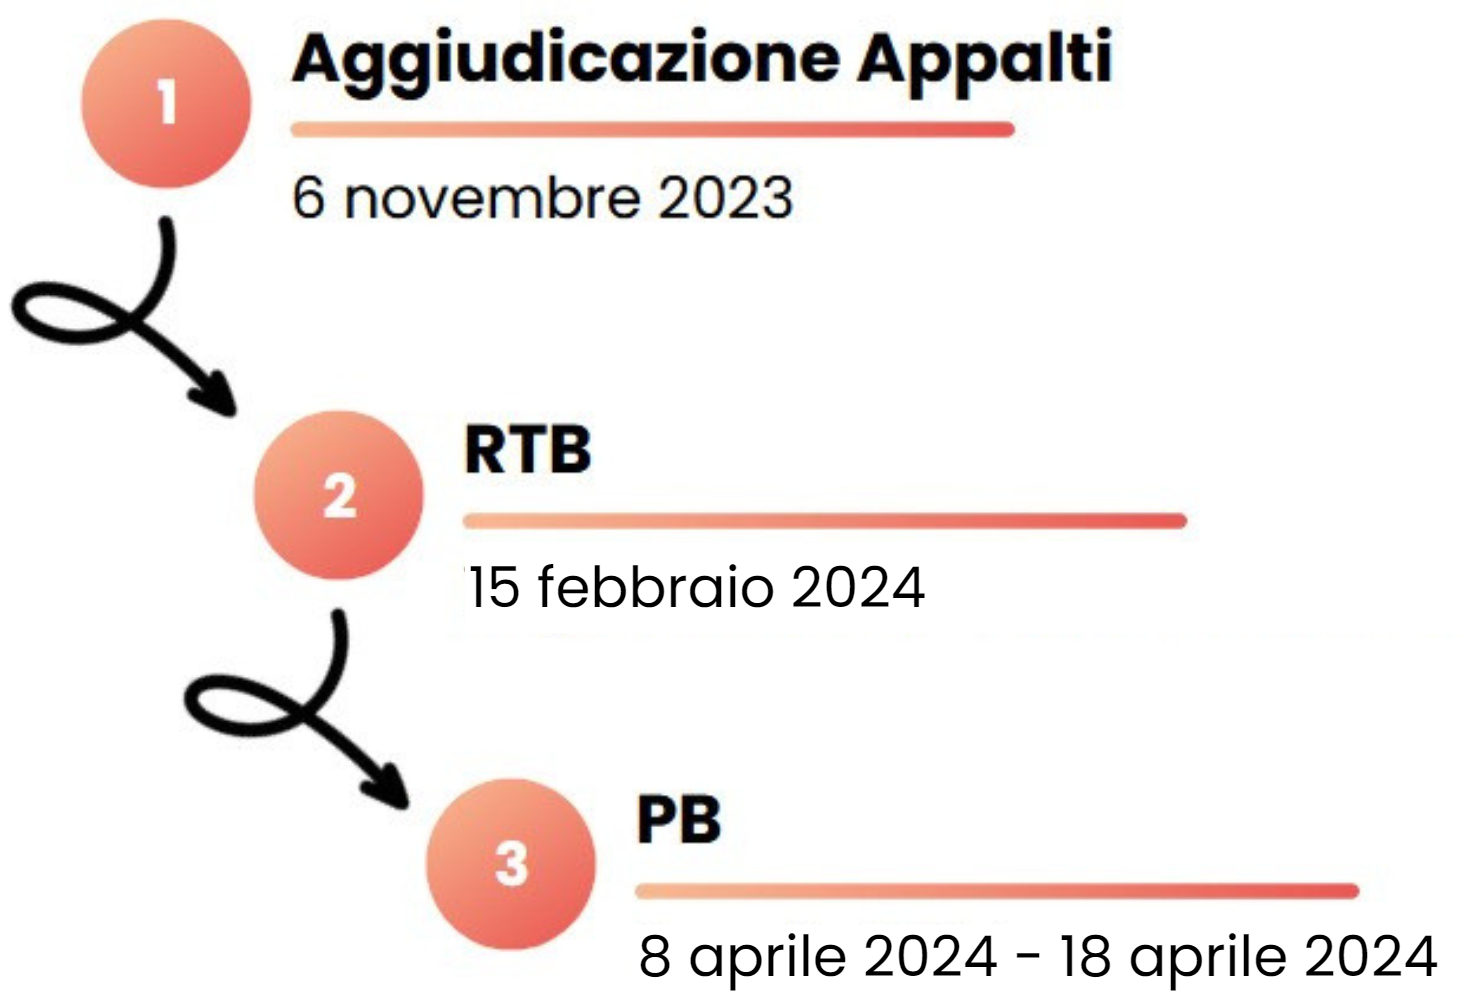
\includegraphics[width=10cm]{calendario di massima.png}
        \caption{Grafico calendario di massima - stesura 2024-04-07}
    \end{figure}
\begin{comment}    
{\renewcommand{\arraystretch}{1.5}
\begin{table}[H]
\begin{tabularx}{\textwidth}{X|X}
\textbf{Revisione} & \textbf{Data} \\
\hline
Requirements \& Technology Baseline & \color{red} Periodo da $2023-12-15$ a $2023-12-20$ \color{black}\\
\hline
Product Baseline &  $2024-04-08$\\

\end{tabularx}
\caption{Tabella calendario di massima - stesura 2024-02-10}
\end{table}}
\end{comment}
\newpage
\section{Stima dei costi di realizzazione}
In questa sezione vengono riportate le stime dei costi e degli impegni orari alla luce di quanto analizzato nelle sezioni di \hyperref[section:Rischi]{\textbf{Rischi e mitigazione}} e \hyperref[section:Pianificazione]{\textbf{Pianificazione}}.

\subsection{Preventivo ore}
A differenza di quanto visto nel Preventivo costi riportato nei documenti forniti alla pre-sentazione della candidatura, la stima dei costi di realizzazione viene modificata. Il preventivo viene riformulato al ribasso, a seguito di diverse riflessioni e considerazioni.\\
Nel corso dei primi periodi è stata ponderata attentamente la suddivisione delle ore proposta in sede di candidatura e sono stati consolidati i seguenti punti critici:
\begin{itemize}
    \item Il team converte alcune ore disponibili in eccesso di Progettista in ore di Analista a parità di costo;
    \item Il team converte alcune ore disponibili in eccesso di Progettista in ore di Ammini-stratore andando a ridurre il costo preventivato;
    \item Il team converte alcune ore disponibili in eccesso di Responsabile in ore di Pro-gettista e Programmatore gi andando a ridurre il costo preventivato.
\end{itemize}
Questi cambiamenti riflettono una maggiore importanza posta sul lavoro di analisi dei requisiti, di amministrazione, di progettista e programmatore rispetto a quanto preventivato a inizio progetto.

\renewcommand{\arraystretch}{1.2}
\begin{table}[H]
\begin{tabularx}{\textwidth}{c|X|X|X|X|X|X|X}
        \textbf{Membri} & $\operatorname{\textbf{Re}}$ & $\mathrm{\textbf{Am}}$ & \textbf{An} & \textbf{Proj} & \textbf{Prgm} & \textbf{Ver} & \textbf{Tot} \\
        \hline Bresolin G. & 9 & 9 & 10 & 11 & 31 & 24 & 94 \\
        \hline Ciriolo I. & 11 & 13 & 12 & 12 & 27 & 19 & 94 \\
        \hline Campese M. & 6 & 10 & 11 & 14 & 28 & 25 & 94 \\
        \hline Dugo A.   & 11 & 9 & 10 & 12 & 28 & 24 & 94 \\
        \hline Feltrin E. & 7 & 9 & 10 & 13 & 30 & 25 & 94 \\
        \hline Michelon R. & 6 & 10 & 11 & 12 & 31 & 24 & 94 \\
        \hline Orlandi G. & 9 & 9 & 9 & 13 & 26 & 28 & 94 
    \end{tabularx}
    \caption{Distribuzione ore - stesura 2024-02-10}
    \end{table}

\subsubsection{Schema a torta di distribuzione ore ruoli}
Di seguito viene illustrata la redistribuzione delle ore nei ruoli di progetto.
    \begin{figure}[H]
        \centering               
     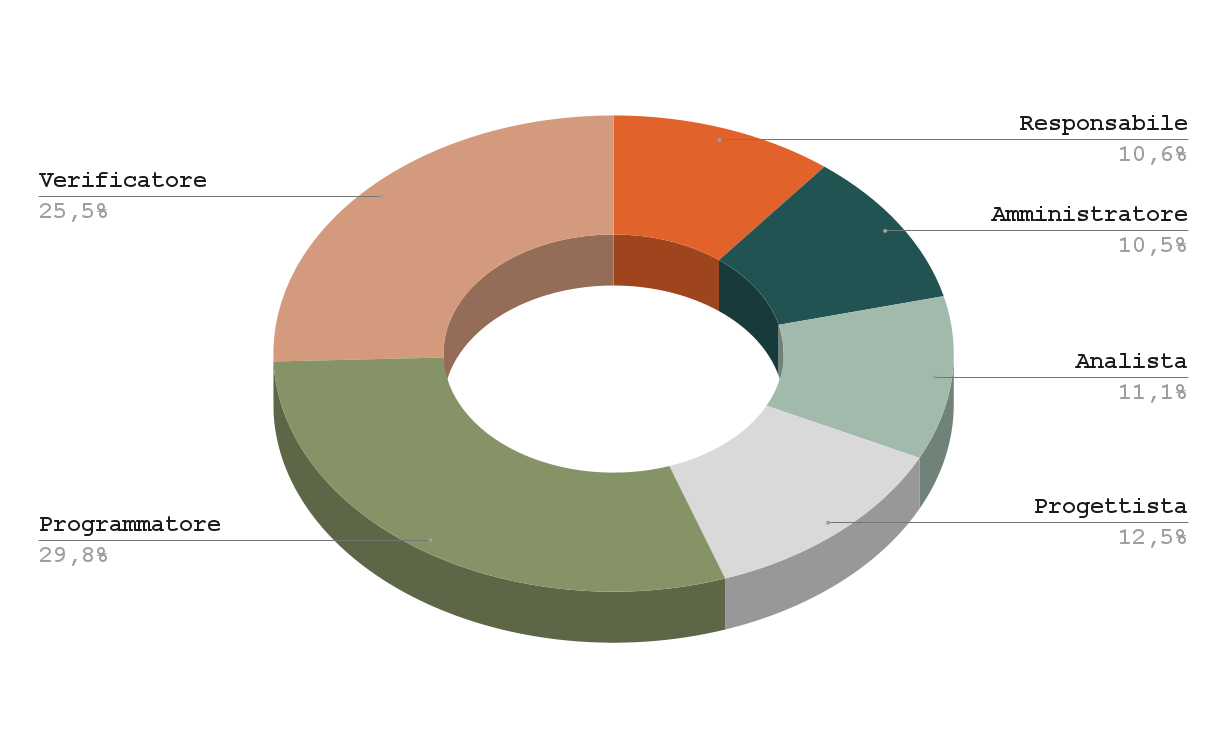
\includegraphics[width=14cm]{tortaPreventivoCosti.png}
         \caption{Grafico ore percentuali - stesura 2024-02-10}
    \end{figure}

\renewcommand{\arraystretch}{1.2}
\begin{center}
\begin{table}[H]
    \begin{tabular}{l|c|c|c|c}
     \textbf{Ruoli} & \textbf{Costo Orario} & \textbf{Ore per Ruolo} & \quantities{\textbf{Ore Medie per}\\\textbf{Membro}} & \textbf{Percentuale Ore} \\
    \hline Responsabile  & 30,00\texteuro & 59 & 8.4 & 9.0\% \\
    \hline Amministratore & 20,00\texteuro & 69 & 9.9 & 10.5\%\% \\
    \hline Verificatore  & 15,00\texteuro & 169 & 24.1 & 25.7\% \\
    \hline Progettista  & 25,00\texteuro & 87 & 12.4 & 13.2\% \\
    \hline Programmatore & 15,00\texteuro & 201 & 28.7 & 30.5\% \\
    \hline Analista      & 25,00\texteuro & 73 & 10.42 & 11.1\%\\
    \hline  & \textbf{Totale Costo} & \textbf{Totale Ore} & \quantities{\textbf{Totale Ore per}\\\textbf{Membro}}\\
    \hline  & \cellcolor{primarycolor} 12700,00\texteuro & \cellcolor{primarycolor}658 &\cellcolor{primarycolor} 94 \\
    \end{tabular}
    \caption{Costo totale - stesura 2024-02-10}
    \end{table}
\end{center}
\subsection{Consuntivo ore}
A seguito di alcune considerazioni dei consuntivi di periodo il team ha rispariamo 250,00\texteuro
\renewcommand{\arraystretch}{1.2}
\begin{table}[H]
\begin{tabularx}{\textwidth}{c|X|X|X|X|X|X|X}
        \textbf{Membri} & $\operatorname{\textbf{Re}}$ & $\mathrm{\textbf{Am}}$ & \textbf{An} & \textbf{Proj} & \textbf{Prgm} & \textbf{Ver} & \textbf{Tot} \\
        \hline Bresolin G. & 9 & 9 & 10 & 11 & 31 & 24 & 94 \\
        \hline Ciriolo I. & 11 & 13 & 12 & 12 & 23 & 19 & 90 \\
        \hline Campese M. & 6 & 10 & 11 & 14 & 26 & 25 & 92 \\
        \hline Dugo A.   & 11 & 9 & 10 & 12 & 28 & 24 & 94 \\
        \hline Feltrin E. & 7 & 9 & 10 & 12 & 30 & 23 & 91 \\
        \hline Michelon R. & 6 & 10 & 11 & 12 & 31 & 24 & 94 \\
        \hline Orlandi G. & 9 & 9 & 9 & 13 & 19 & 28 & 87 
    \end{tabularx}
    \caption{Distribuzione ore - stesura 2024-04-07}
    \end{table}
\subsubsection{Schema a torta di consuntivo ore ruoli}
Di seguito viene illustrata la redistribuzione delle ore nei ruoli di progetto dopo l'ultimo consuntivo.
    \begin{figure}[H]
        \centering               
     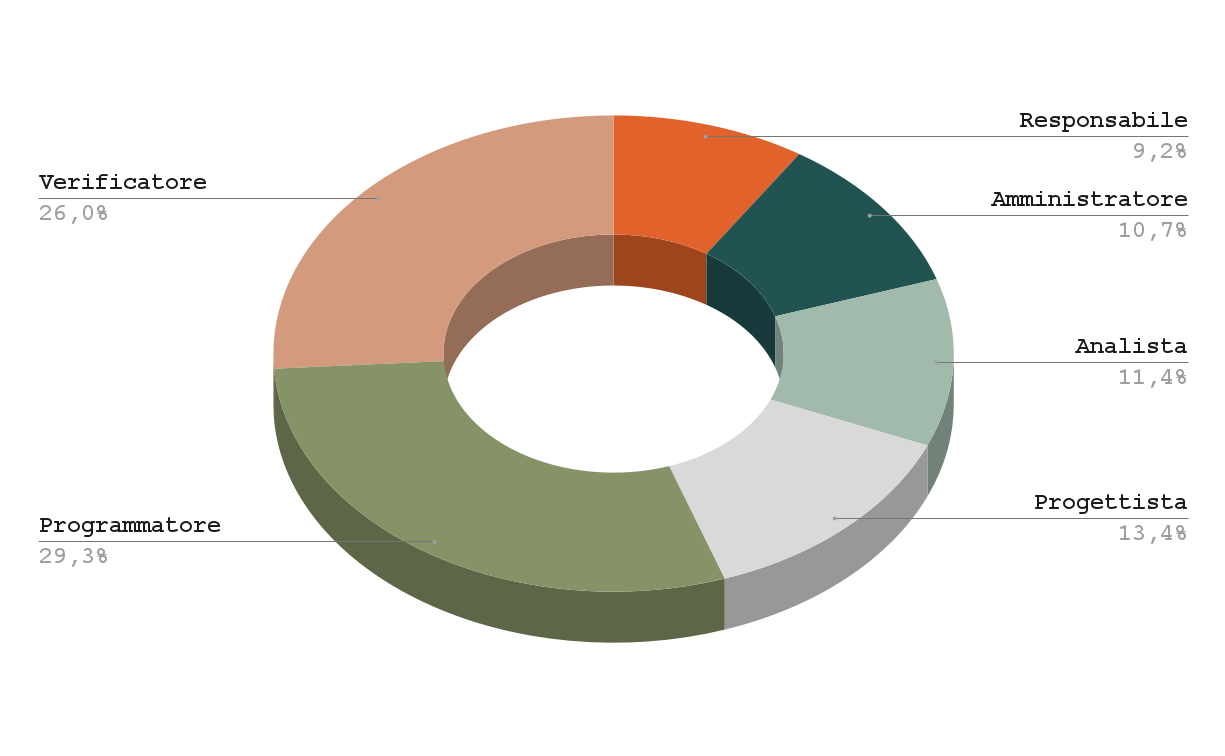
\includegraphics[width=14cm]{tortaConsuntivoCosti.png}
         \caption{Grafico ore utilizzate - stesura 2024-04-07}
    \end{figure}

\renewcommand{\arraystretch}{1.2}
\begin{center}
\begin{table}[H]
    \begin{tabular}{l|c|c|c|c}
     \textbf{Ruoli} & \textbf{Costo Orario} & \textbf{Ore per Ruolo} & \quantities{\textbf{Ore Medie per}\\\textbf{Membro}} & \textbf{Percentuale Ore} \\
    \hline Responsabile  & 30,00\texteuro & 59 & 8.4 & 9.2\% \\
    \hline Amministratore & 20,00\texteuro & 69 & 9.9 & 10.7\%\% \\
    \hline Verificatore  & 15,00\texteuro & 167 & 24.2 & 26.0\% \\
    \hline Progettista  & 25,00\texteuro & 86 & 12.3 & 13.4\% \\
    \hline Programmatore & 15,00\texteuro & 188 & 26.8 & 29.3\% \\
    \hline Analista      & 25,00\texteuro & 73 & 10.4 & 11.4\%\\
    \hline  & \textbf{Totale Costo} & \textbf{Totale Ore} & \quantities{\textbf{Totale Ore per}\\\textbf{Membro}}\\
    \hline  & \cellcolor{primarycolor} 12450,00\texteuro & \cellcolor{primarycolor}642 &\cellcolor{primarycolor} 92 \\
    \end{tabular}
    \caption{Costo totale - stesura 2024-04-07}
    \end{table}
\end{center}
\newpage
%    PIANIFICAZIONE
\section{Pianificazione e modello di sviluppo}
\label{section:Pianificazione}

Il team decide di adottare il modello di sviluppo \textit{Agile\pg} 
promuovendo un approccio incrementale al lavoro; questo consentirà di suddividere il progetto in compiti più gestibili, ovvero \textit{sprint}, ciascuno dei quali produrrà risultati funzionanti. Questo consente al team di progetto di reagire ai cambiamenti in modo più efficace.
Il team definisce in seguito una pianificazione generale che verrà approfondita prima di ogni sprint.
I periodi individuati sono \textit{sprint} di 14 giorni con conseguente rotazione dei ruoli assunti dai componenti del gruppo.\\
Questo tipo di pianificazione permette di avere un orizzonte temporale limitato, sebbene vi sia una pianificazione dell'intero periodo del progetto; ciò aiuta nel caso in cui vengano riscontrate difficoltà che causano danni ad attività che dipendono le une dalle altre. In questi casi è quindi possibile contenere i danni e riorganizzare le attività nel periodo successivo.

\subsection{Requirements and Technology Baseline}
Questo periodo antecedente la revisione \textit{RTB\pg} di progetto si focalizza sulla preparazione dei documenti (Analisi dei requisiti, Piano di progetto, Piano di qualifica, ampliamento Norme di progetto) e sulla creazione del \textit{Proof of Concept\pg} per il progetto.
%\vspace{2em}
\subsubsection{Periodo 1: da 2023-11-07 a 2023-11-21}
Questo primo periodo segue l'assegnazione dei capitolati e viene utilizzato principalmente per configurare l'ambiente di lavoro, le norme e per studiare i casi d'uso e perseguire l'analisi dei requisiti del progetto. Infine lo \textit{sprint} si concentra sullo studio e selezione di tecnologie utili allo sviluppo del progetto.
\subsubsubsection{Obiettivi}
\begin{itemize}
    \item Stesura e ampliamento delle Norme di progetto;
    \item Prima stesura Analisi dei requisiti;
    \item Automazione \textit{versionamento\pg};
    \item Manutenzione ambiente di lavoro;
    \item Software selection;
    \item Verbali delle riunioni.
        
\end{itemize}
%\paragraph{Diagramma di Gantt}
\vspace{1em}

 \begin{figure}[H]
        \centering        
        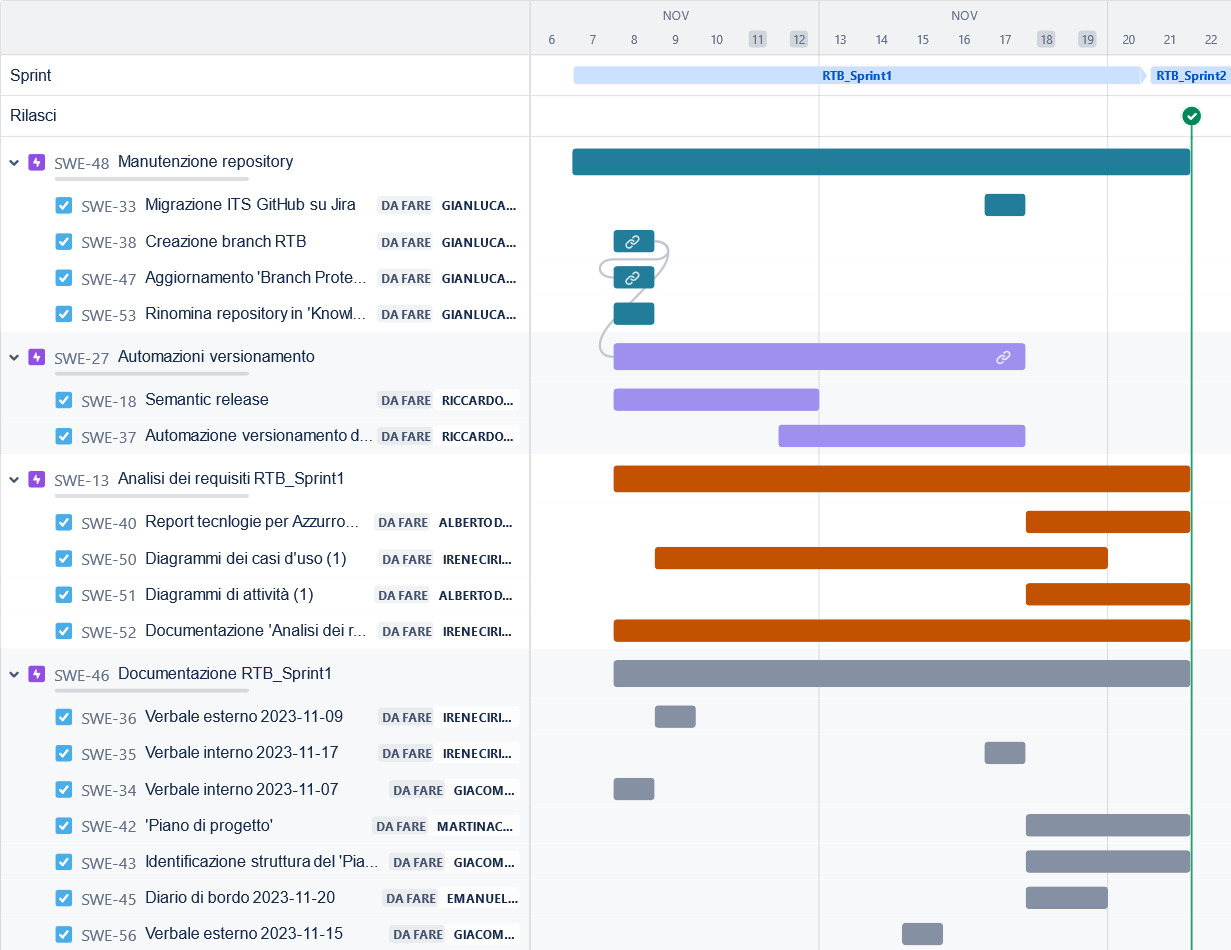
\includegraphics[width=15.5cm]{gantt/ganttPeriodo1.png}
        \caption{Diagramma di Gantt Periodo 1 }
    \end{figure}
\newpage
%\vspace{2em}
\subsubsection{Periodo 2: da 2023-11-21 a 2023-12-05}
In questo periodo le ore di lavoro sono concentrate nella creazione di un \textit{PoC\pg} richiesto dall'azienda e nell'ampliamento e miglioramento della documentazione necessaria per guidare l'avanzamento del progetto.
\subsubsubsection{Obiettivi}
\begin{itemize}
    \item Progettazione PoC;
    \item \textit{Codifica\pg} PoC;
    \item Prosecuzione stesura Analisi dei requisiti;
    \item Migliorie Norme di progetto e Piano di progetto;
    \item Stesura correttiva Piano di qualifica;
    \item Verbali delle riunioni.
  
\end{itemize}
%\paragraph{Diagramma di Gantt}
\vspace{1em}

 \begin{figure}[H]
        \centering        
        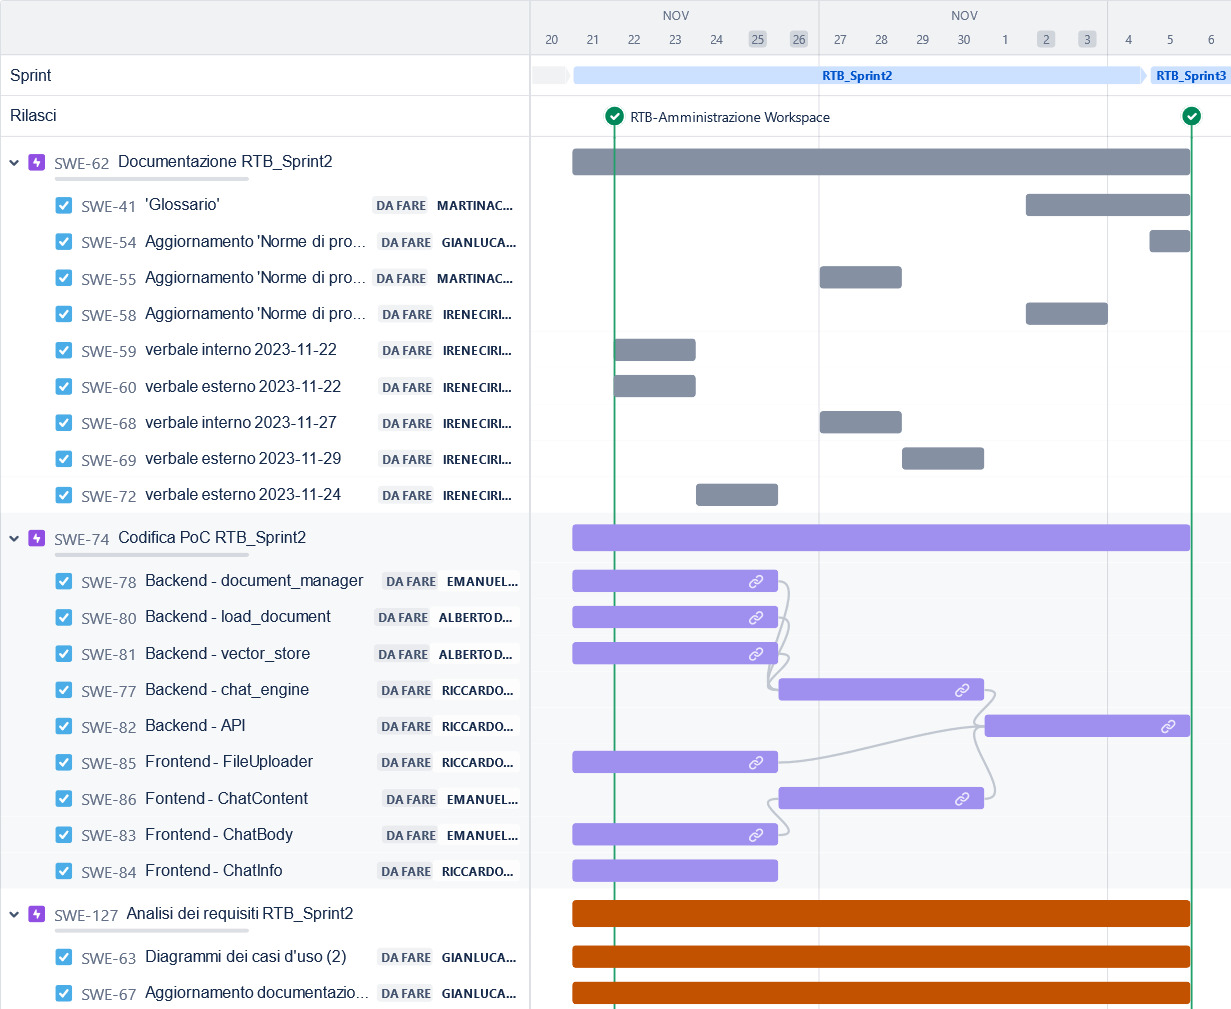
\includegraphics[width=15.5cm]{gantt/ganttPeriodo2.png}
        \caption{Diagramma di Gantt Periodo 2 }
    \end{figure}
\newpage
\subsubsection{Periodo 3: da 2023-12-05 a 2023-12-19}
\subsubsubsection{Obiettivi}
\begin{itemize}
    \item \textit{Refactoring\pg} codice PoC;
    \item Refactoring architettura PoC;
    \item Correzione e conclusione stesura Analisi dei requisiti;
    \item Migliorie Norme di progetto e ampliamento Piano di progetto alla luce del Piano di Qualifica;
    \item Ampliamento sostanziale del Piano di qualifica;
    \item Verbali delle riunioni.
\end{itemize}
\begin{figure}[H]
    \centering        
    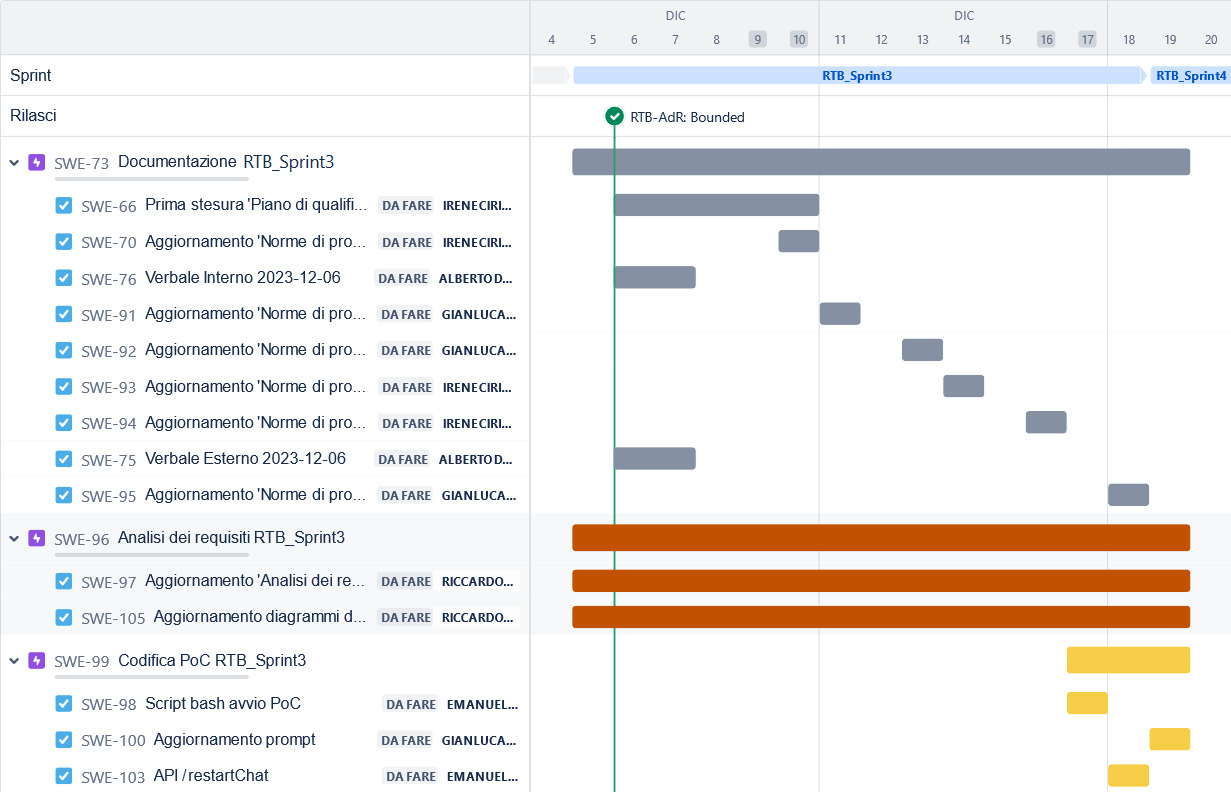
\includegraphics[width=15.5cm]{gantt/ganttPeriodo3.png}
    \caption{Diagramma di Gantt Periodo 3 }
\end{figure}
\newpage
\subsubsection{Periodo 4: da 2023-12-19 a 2024-01-02}
\subsubsubsection{Obiettivi}
\begin{itemize}
    \item Refactoring totale delle Norme di progetto;
    \item Aggiornamento Piano di qualifica;
    \item Miglioramento codice Poc;
    \item Verbali delle riunioni.
\end{itemize}
\begin{figure}[H]
    \centering        
    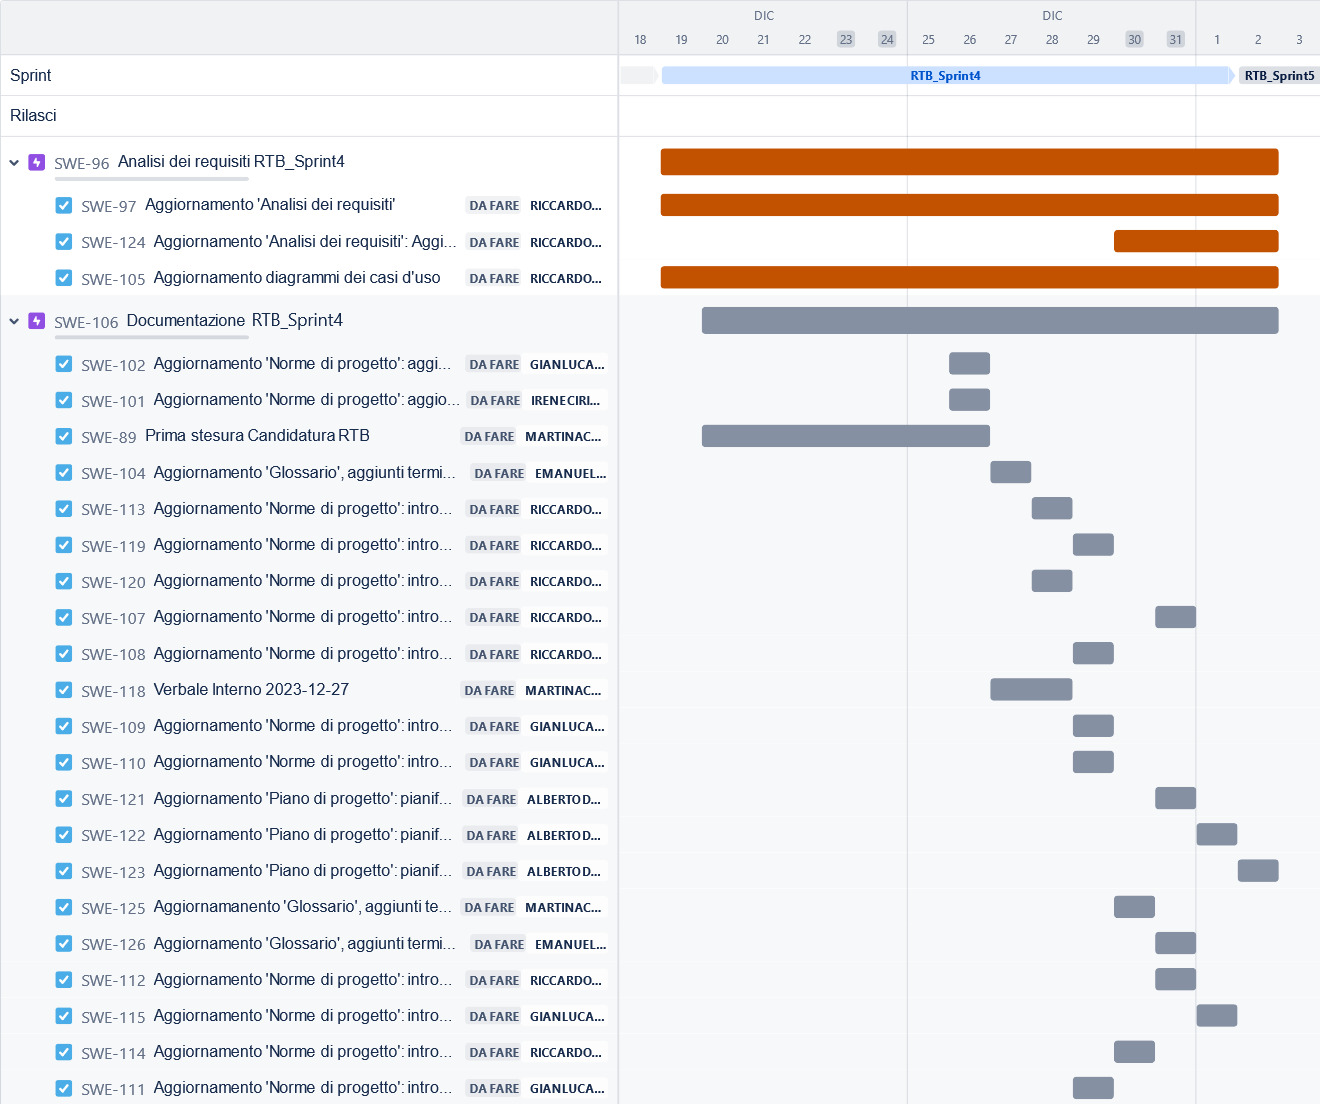
\includegraphics[width=15.5cm]{gantt/ganttPeriodo4.png}
    \caption{Diagramma di Gantt Periodo 4}
\end{figure}

\subsubsection{Periodo 5: da 2024-01-02 a 2024-01-16}
\subsubsubsection{Obiettivi}
\begin{itemize}
    \item Aggiornamento Piano di qualifica;
    \item Aggiornamento Piano di progetto;
    \item Aggiornamento Analisi dei requisiti;
    \item Presentazione candidatura prima fase di revisione RTB;
    \item Verbali delle riunioni.
\end{itemize}
\begin{figure}[H]
    \centering        
    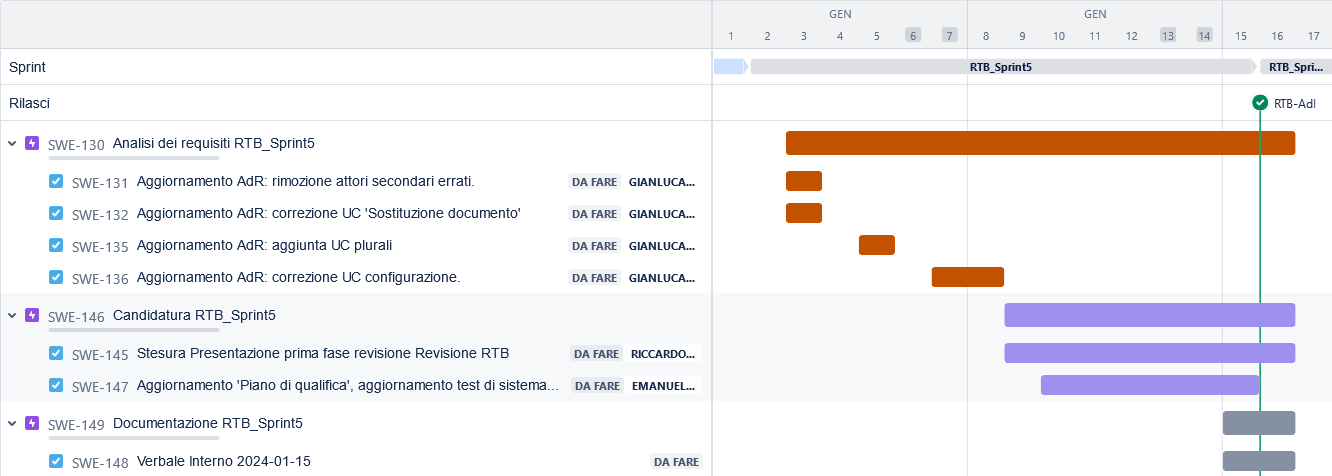
\includegraphics[width=15.5cm]{gantt/ganttPeriodo5.png}
    \caption{Diagramma di Gantt Periodo 5}
\end{figure}

\subsubsection{Periodo 6: da 2024-01-16 a 2024-01-30}
%
\subsubsubsection{Obiettivi}
\begin{itemize}
    \item Aggiornamento Piano di progetto;
    \item Verbali delle riunioni;
    \item Colloquio con il Professore Cardin R. per la revisione RTB.
\end{itemize}
\begin{figure}[H]
    \centering        
    \includegraphics[width=15.5cm]{gantt/ganttPeriodo6.png}
    \caption{Diagramma di Gantt Periodo 6}
\end{figure}

\subsubsection{Periodo 7: da 2024-01-30 a 2024-02-13}
%
\subsubsubsection{Obiettivi}
\begin{itemize}
    \item Inizio progettazione;
    \item Progettazione con Azzurro Digitale;
    \item Colloquio con il Professore Vardanega T. per la revisione RTB;
    \item Aggiornamento Piano di qualifica;
    \item Aggiornamento Piano di progetto;
    \item Verbali delle riunioni.
\end{itemize}
\begin{figure}[H]
    \centering        
    \includegraphics[width=15.5cm]{gantt/ganttPeriodo7.png}
    \caption{Diagramma di Gantt Periodo 7}
\end{figure}

\subsection{Product Baseline}
Questo periodo antecedente la revisione \textit{PB\pg} di progetto si focalizza sulla preparazione dei documenti (Analisi dei requisiti, Piano di progetto, Piano di qualifica, Norme di progetto, Specifica tecnica, Manuale utente) e sulla creazione del \textit{Minimum Viable Product\pg} per il progetto.

\subsubsection{Periodo 8: da 2024-02-13 a 2024-02-27}
%
\subsubsubsection{Obiettivi}
\begin{itemize}
    \item Continuazione progettazione logica e di dettaglio;
    \item Progettazione di dettaglio;
    \item Inizio stesura Specifica tecnica;
    \item Eventuali correzioni alla documentazione post colloquio;
    \item Aggiornamento Piano di qualifica;
    \item Aggiornamento Piano di progetto;
    \item Verbali delle riunioni.
\end{itemize}


\begin{figure}[H]
    \centering        
    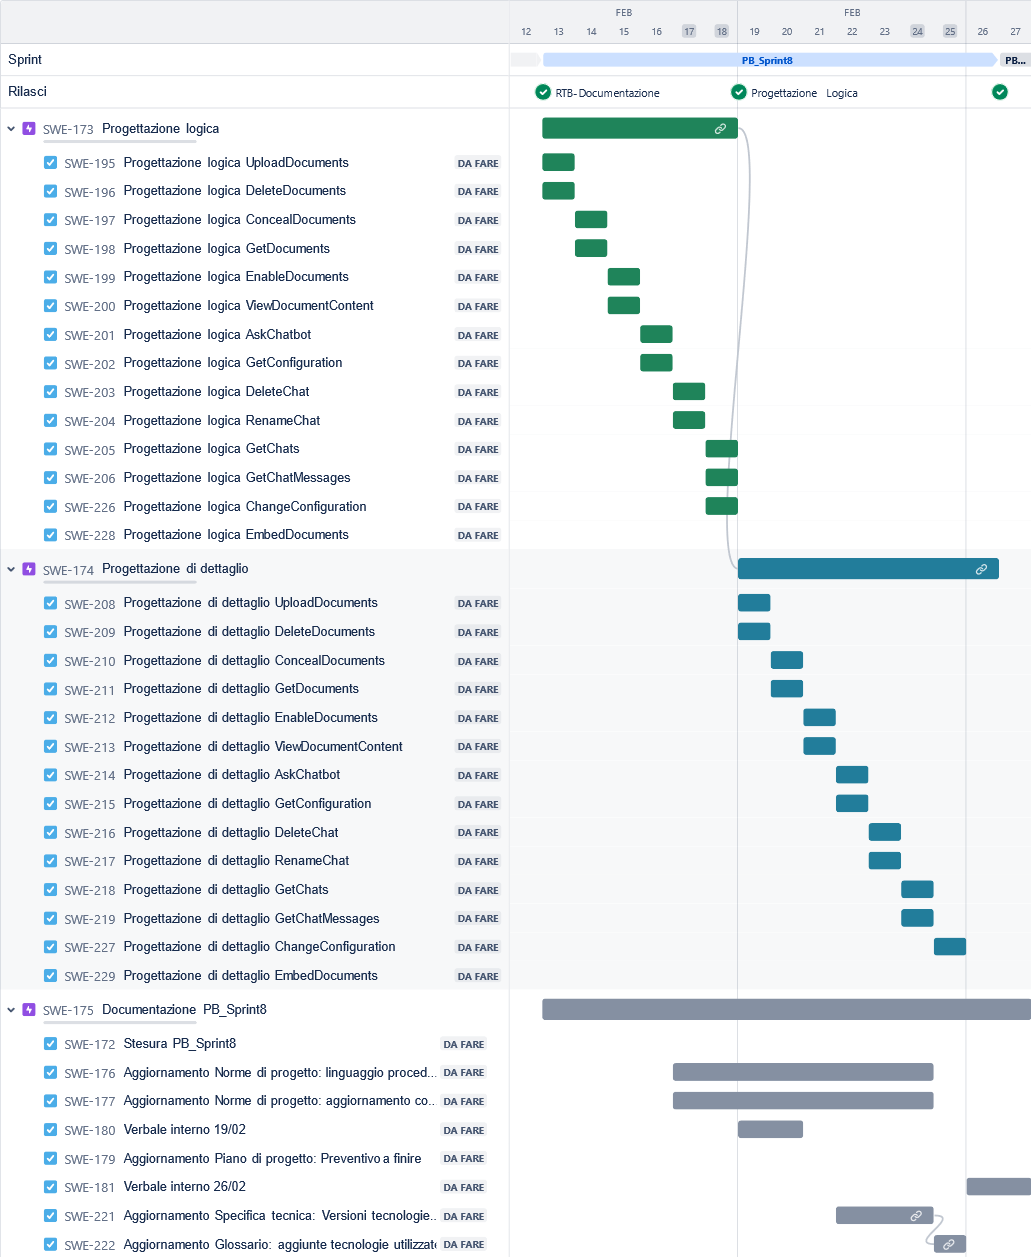
\includegraphics[width=15.5cm]{gantt/ganttPeriodo8.png}
    \caption{Diagramma di Gantt Periodo 8}
\end{figure}


\subsubsection{Periodo 9: da 2024-02-27 a 2024-03-12}
%
\subsubsubsection{Obiettivi}
\begin{itemize}
    \item Programmazione backend;
    \item Test di unità;
    \item Documentazione relativa al codice;
    \item Aggiornamento Piano di qualifica;
    \item Aggiornamento Piano di progetto;
    \item Verbali delle riunioni.
\end{itemize}

\begin{figure}[H]
    \centering        
    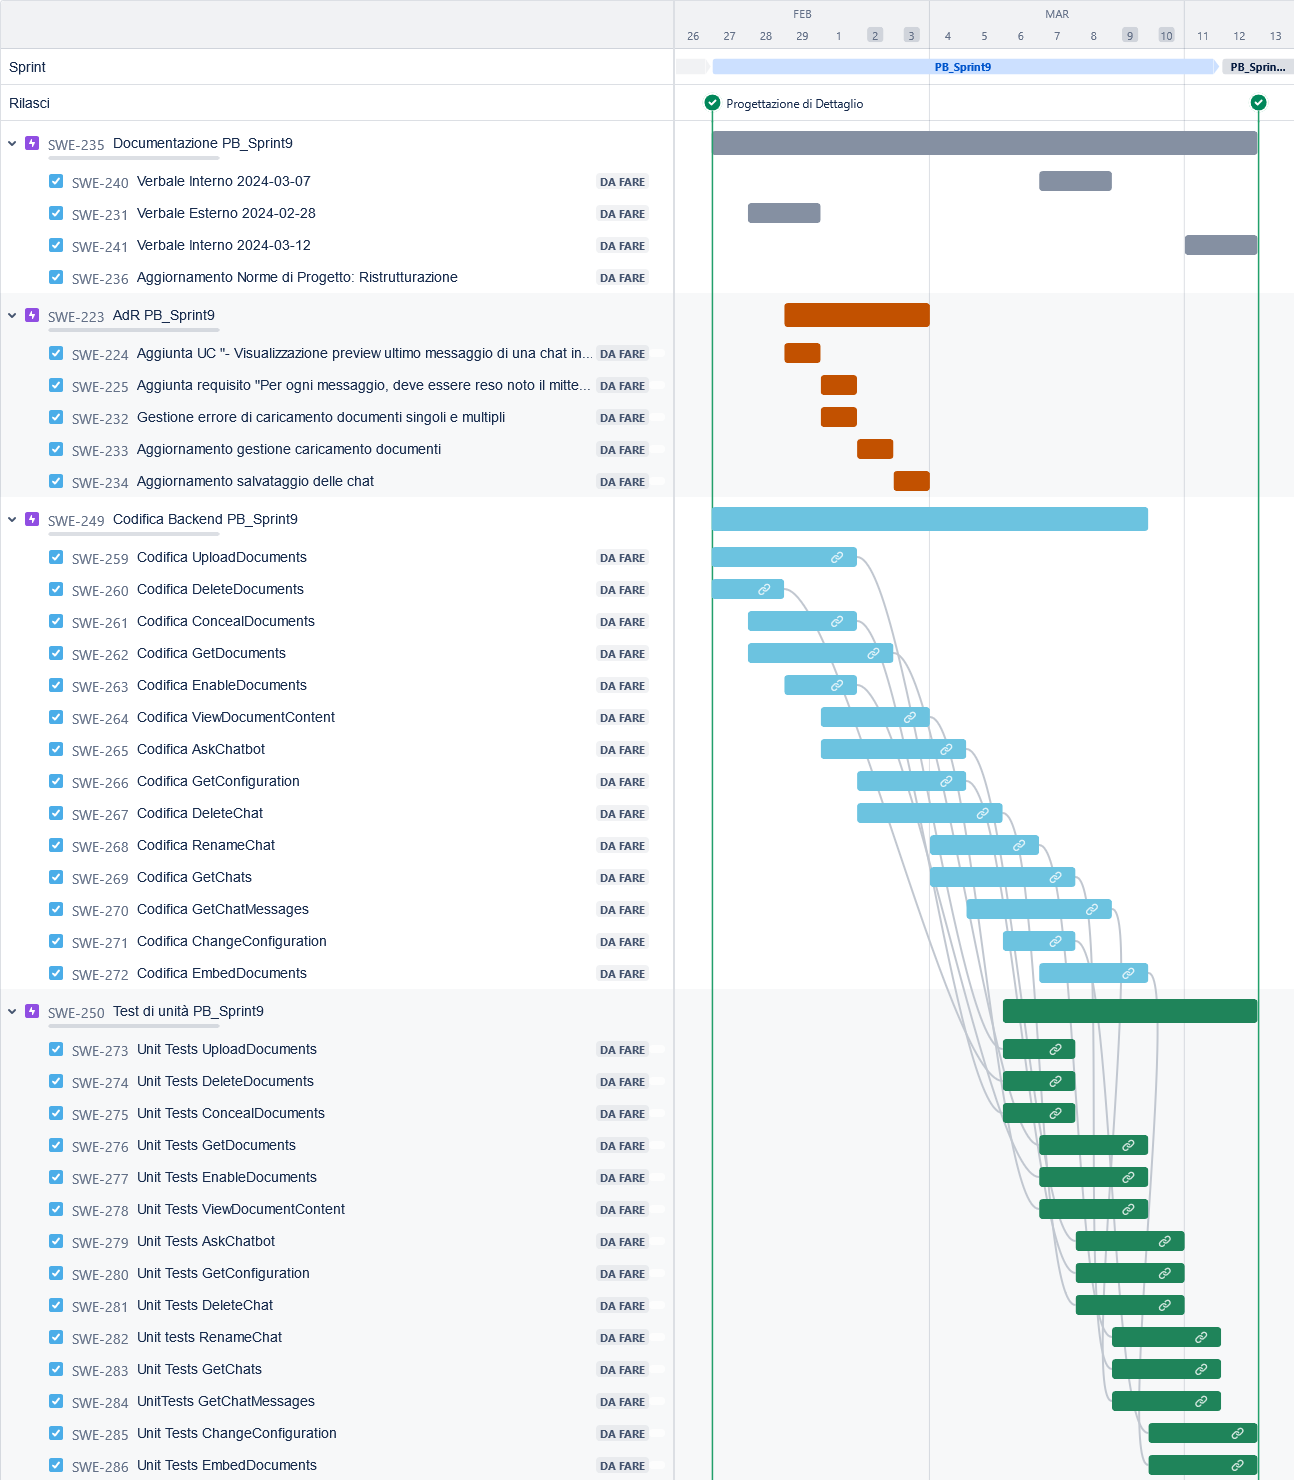
\includegraphics[width=15.5cm]{gantt/ganttPeriodo9.png}
    \caption{Diagramma di Gantt Periodo 9}
\end{figure}

\subsubsection{Periodo 10: da 2024-03-12 a 2024-03-26}
%
\subsubsubsection{Obiettivi}
\begin{itemize}
    \item Programmazione frontend;
    \item Test di integrazione;
    \item Stesura Manuale Utente;
    \item Continuazione stesura Specifica tecnica;
    \item Aggiornamento Piano di qualifica;
    \item Aggiornamento Piano di progetto;
    \item Verbali delle riunioni.
\end{itemize}

\begin{figure}[H]
    \centering        
    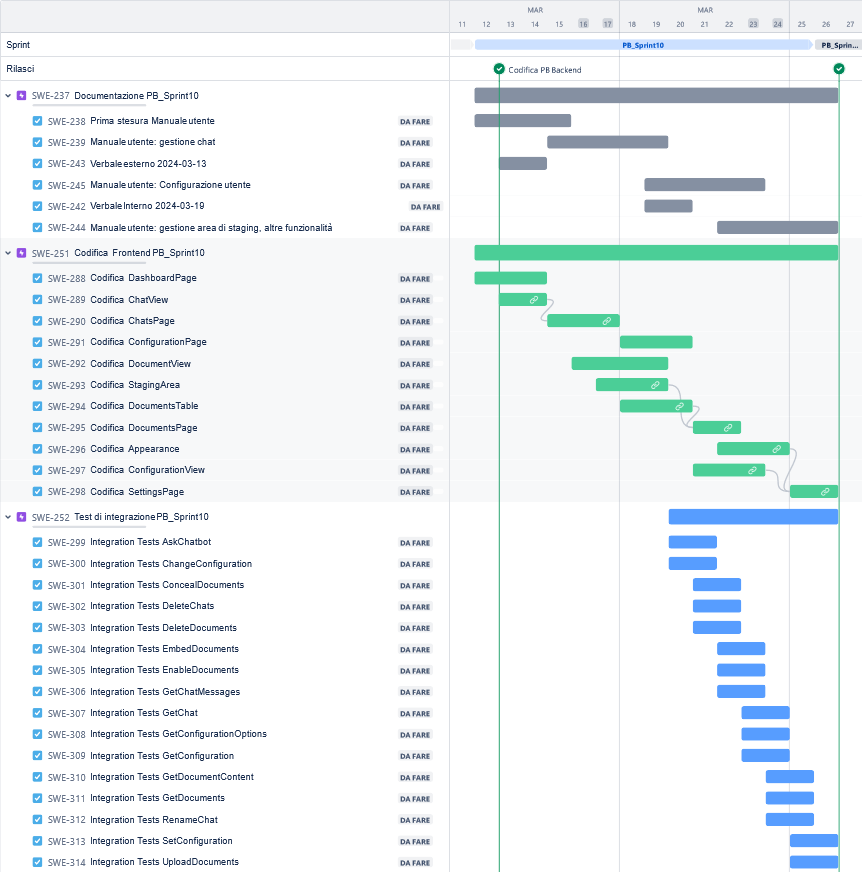
\includegraphics[width=15.5cm]{gantt/ganttPeriodo10.png}
    \caption{Diagramma di Gantt Periodo 10}
\end{figure}

\subsubsection{Periodo 11: da 2024-03-26 a 2024-04-08}
%
\subsubsubsection{Obiettivi}
\begin{itemize}
    \item Conclusione Programmazione;
    \item Test di sistema;
    \item Conclusione stesura Manuale Utente;
    \item Conclusione stesura Specifica tecnica;
    \item Documentazione relativa al codice;
    \item Conclusione Piano di qualifica;
    \item Conclusione Piano di progetto;
    \item Verbali delle riunioni.
\end{itemize}
\begin{figure}[H]
    \centering        
    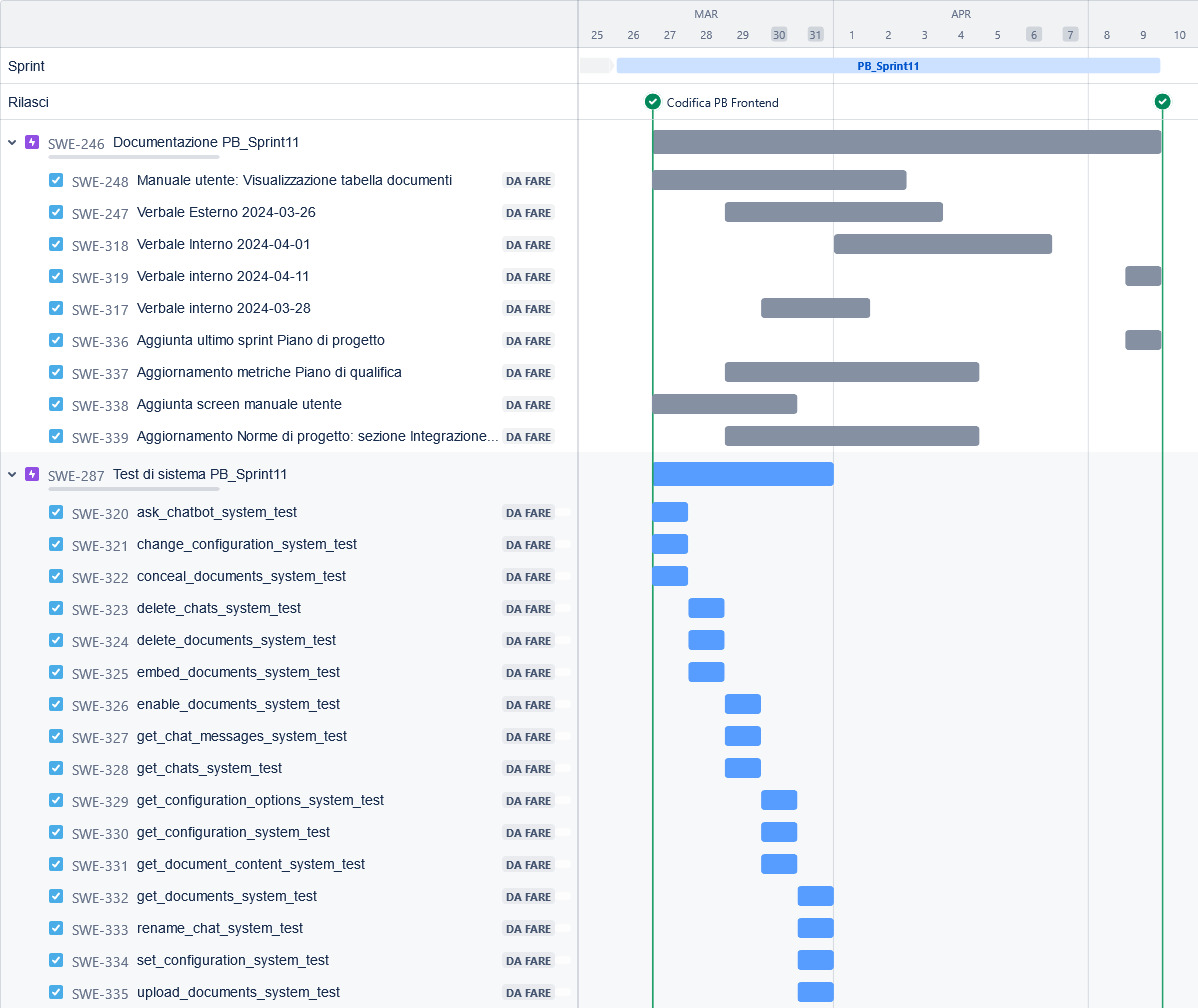
\includegraphics[width=15.5cm]{gantt/ganttPeriodo11.jpeg}
    \caption{Diagramma di Gantt Periodo 11}
\end{figure}

\newpage
% PREVENTIVO
\section{Preventivo}
Ogni membro del team mette a disposizione le sue conoscenze e le 94 ore produttive ciascuno, divise nei vari ruoli. Il preventivo è stato calcolato in base al costo orario di ciascun componente, e in base alla nostra previsione di attività da svolgere in ogni sprint. Di seguito, vengono dettagliati gli aspetti di ciascun incremento e il relativo costo. La distribuzione dei ruoli tra i membri è stata equa, offrendo a ognuno l'opportunità di sperimentare diverse mansioni. \textit{Abbreviazioni\pg} specifiche sono utilizzate nelle tabelle per brevità:
\begin{itemize}
    \item Re: Responsabile;
    \item Am: Amministratore;
    \item An: Analista;
    \item Proj: Progettista;
    \item Prgm: Programmatore;
    \item Ver: Verificatore.
\end{itemize}
Nelle tabelle sottostanti relative al preventivo è possibile trovare una cella colorata per ogni membro del team, la quale si riferisce al ruolo che il membro stesso assumerà.
% SPRINT 1 PREVENTIVO
\subsection{Sprint 1: da 2023-11-07 a 2023-11-21}

Di seguito, la distribuzione delle ore del primo sprint; ogni componente del gruppo rivestirà i ruoli come segue:
\begin{table}[H]
\begin{tabularx}{\textwidth}{c|X|X|X|X|X|X|X}
        \textbf{Membri} & $\operatorname{\textbf{Re}}$ & $\mathrm{\textbf{Am}}$ & \textbf{An} & \textbf{Proj} & \textbf{Prgm} & \textbf{Ver} & \textbf{Totale} \\
        \hline Bresolin G. & 0 & \cellcolor{primarycolor}4 & 0 & 0 & 0 & 0 & 4 \\
        \hline Ciriolo I.  & 0 & 0 & \cellcolor{primarycolor}6 & 0 & 0 & 1 & 7 \\
        \hline Campese M.  & 0 & 0 & 2 & 0 & 0 & \cellcolor{primarycolor}8 & 10 \\
        \hline Dugo A.     & 0 & \cellcolor{primarycolor}4 & 0 & 0 & 0 & 0 & 4 \\
        \hline Feltrin E.  & \cellcolor{primarycolor}8 & 1 & 0 & 0 & 0 & 0 & 9 \\
        \hline Michelon R. & 0 & \cellcolor{primarycolor}6 & 0 & 0 & 0 & 0 & 6 \\
        \hline Orlandi G.  & 0 & 0 & \cellcolor{primarycolor}3 & 0 & 0 & 1 & 4 \\
        \hline
        \textbf{Totale ruolo} & 8 & 15 & 11 & 0 & 0 & 10 & 44 
    \end{tabularx}
    \caption{Preventivo ore - Sprint 1}
    \end{table}

La tabella è riassunta dal seguente istogramma:
 \begin{figure}[H]
        \centering        
        \includegraphics[width=15.5cm]{istogrammi/istogramma_1_periodo.png}
        \caption{Sprint 1 - Istogramma della ripartizione oraria dei ruoli. }
    \end{figure}
 
In questo incremento, il costo per ogni ruolo sarà come da tabella:
\renewcommand{\arraystretch}{1.5}
\begin{table}[H]
\centering
\begin{tabularx}{0.42\textwidth}{c|c|c}

\textbf{Ruolo} & \textbf{Ore} & \textbf{Costo}\\
\hline
\textbf{Responsabile} & 8 & 240,00\texteuro\\
\hline
\textbf{Amministratore} & 15 & 300,00\texteuro \\
\hline
\textbf{Analista} & 11 & 275,00\texteuro \\
\hline
\textbf{Progettista} & 0 & 0\texteuro\\
\hline
\textbf{Programmatore} & 0 & 0\texteuro \\ 
\hline
\textbf{Verificatore} & 10 & 150,00\texteuro \\ 
\hline
\rowcolor{primarycolor}
\textbf{Totale} & 44 & 965,00\texteuro \\
\end{tabularx}
%}
\caption{Preventivo costi - Sprint 1}
\end{table}

La tabella è riassunta dal seguente aereogramma:
 \begin{figure}[H]
        \centering        
        \includegraphics[width=15.5cm]{aereogrammi/areogramma_1_periodo.png}
        \caption{Sprint 1 - Areogramma della ripartizione oraria dei ruoli. }
    \end{figure}



%SPRINT 2 PREVENTIVO

\subsection{Sprint 2: da 2023-11-21 a 2023-12-05 }
Di seguito, la distribuzione delle ore del secondo sprint; ogni componente del gruppo rivestirà i ruoli come segue:
\begin{table}[H]
\begin{tabularx}{\textwidth}{c|X|X|X|X|X|X|X}
        \textbf{Membri} & $\operatorname{\textbf{Re}}$ & $\mathrm{\textbf{Am}}$ & \textbf{An} & \textbf{Proj} & \textbf{Prgm} & \textbf{Ver} & \textbf{Totale} \\
        \hline Bresolin G. & 0 & 1 & \cellcolor{primarycolor}6 & 0 & 0 & 0 & 7 \\
        \hline Ciriolo I.  & \cellcolor{primarycolor}7 & 0 & 0 & 0 & 0 & 1 & 8 \\
        \hline Campese M.  & 0 & \cellcolor{primarycolor}5 & 2 & 0 & 0 & 1,5 & 8,5 \\
        \hline Dugo A.     & 0 & 0 & 2 & \cellcolor{primarycolor}2 & 9 & 0 & 13 \\
        \hline Feltrin E.  & 0 & 0 & 0 & 0 & \cellcolor{primarycolor}11 & 0 & 11 \\
        \hline Michelon R. & 0 & 0 & 2 & 1 & \cellcolor{primarycolor}13 & 0 & 16 \\
        \hline Orlandi G.  & 0 & 0 & 0 & 0 & 0 & \cellcolor{primarycolor}7 & 7 \\
        \hline
        \textbf{Totale ruolo} & 7 & 6 & 12 & 3 & 33 & 9,5 & 70,5 
    \end{tabularx}
    \caption{Preventivo ore - Sprint 2}
    \end{table}
La tabella è riassunta dal seguente istogramma:
 \begin{figure}[H]
        \centering        
        \includegraphics[width=15.5cm]{istogrammi/istogramma_2_periodo.png}
        \caption{Sprint 2 - Istogramma della ripartizione oraria dei ruoli. }
    \end{figure}
In questo incremento, il costo per ogni ruolo sarà come da tabella:
\renewcommand{\arraystretch}{1.5}
\begin{table}[H]
\centering
\begin{tabularx}{0.42\textwidth}{c|c|c}

\textbf{Ruolo} & \textbf{Ore} & \textbf{Costo}\\
\hline
\textbf{Responsabile} & 7 & 210,00\texteuro\\
\hline
\textbf{Amministratore} & 6 & 120,00\texteuro \\
\hline
\textbf{Analista} & 12 & 300,00\texteuro \\
\hline
\textbf{Progettista} & 3 & 75,00\texteuro\\
\hline
\textbf{Programmatore} & 33 & 495,00\texteuro \\ 
\hline
\textbf{Verificatore} & 9,5 & 142,50\texteuro \\ 
\hline
\rowcolor{primarycolor}
\textbf{Totale} & 70,5 & 1342,50\texteuro \\
\end{tabularx}
%}
\caption{Preventivo costi - Sprint 2}
\end{table}
La tabella è riassunta dal seguente aereogramma:
 \begin{figure}[H]
        \centering        
        \includegraphics[width=15.5cm]{aereogrammi/areogramma_2_periodo.png}
        \caption{Sprint 2 - Areogramma della ripartizione oraria dei ruoli. }
    \end{figure}

% SPRINT 3 PREVENTIVO

\subsection{Sprint 3: da 2023-12-05 a 2023-12-19}
Di seguito, la distribuzione delle ore del terzo sprint; ogni componente del gruppo rivestirà i ruoli come segue:
\begin{table}[H]
\begin{tabularx}{\textwidth}{c|X|X|X|X|X|X|X}
        \textbf{Membri} & $\operatorname{\textbf{Re}}$ & $\mathrm{\textbf{Am}}$ & \textbf{An} & \textbf{Proj} & \textbf{Prgm} & \textbf{Ver} & \textbf{Totale} \\
        \hline Bresolin G. & 0 & 0 & 2 & 1 & 0 & \cellcolor{primarycolor}7 & 10 \\
        \hline Ciriolo I.  & 0 & \cellcolor{primarycolor}4 & 1 & 0 & 0 & 3 & 7 \\
        \hline Campese M.  & 0 & 0 & \cellcolor{primarycolor}2 & 0 & 0 & 4 & 6 \\
        \hline Dugo A.     & \cellcolor{primarycolor}6 & 0 & 2 & 0 & 0 & 0 & 8 \\
        \hline Feltrin E.  & 0 & 0 & \cellcolor{primarycolor}8 & 0 & 0 & 0 & 8 \\
        \hline Michelon R. & 0 & 0 & \cellcolor{primarycolor}7 & 0 & 0 & 0 & 7 \\
        \hline Orlandi G.  & 0 & 0 & 3 & 0 & \cellcolor{primarycolor}4 & 0 & 7 \\
        \hline
        \textbf{Totale ruolo} & 6 & 4 & 25 & 1 & 4 & 14 & 54 
    \end{tabularx}
    \caption{Preventivo ore - Sprint 3}
    \end{table}

La tabella è riassunta dal seguente istogramma:
 \begin{figure}[H]
        \centering        
        \includegraphics[width=15.5cm]{istogrammi/istogramma_3_periodo.png}
        \caption{Sprint 3 - Istogramma della ripartizione oraria dei ruoli. }
    \end{figure}

In questo incremento, il costo per ogni ruolo sarà come da tabella:
\renewcommand{\arraystretch}{1.5}
\begin{table}[H]
\centering
\begin{tabularx}{0.42\textwidth}{c|c|c}

\textbf{Ruolo} & \textbf{Ore} & \textbf{Costo}\\
\hline
\textbf{Responsabile} & 6 & 180,00\texteuro\\
\hline
\textbf{Amministratore} & 4 & 80,00\texteuro \\
\hline
\textbf{Analista} & 25 & 625,00\texteuro \\
\hline
\textbf{Progettista} & 1 & 25,00\texteuro\\
\hline
\textbf{Programmatore} & 4 & 60,00 \texteuro \\ 
\hline
\textbf{Verificatore} & 14 & 210,00\texteuro \\ 
\hline
\rowcolor{primarycolor}
\textbf{Totale} & 53 & 1180,00\texteuro \\
\end{tabularx}
%}
\caption{Preventivo costi - Sprint 3}
\end{table}


La tabella è riassunta dal seguente aereogramma:
 \begin{figure}[H]
        \centering        
        \includegraphics[width=15.5cm]{aereogrammi/areogramma_3_periodo.png}
        \caption{Sprint 3 - Areogramma della ripartizione oraria dei ruoli. }
    \end{figure}



%   PERIODO 4

\subsection{Sprint 4: da 2023-12-19 a 2024-01-02}
Di seguito, la distribuzione delle ore del quarto sprint; ogni componente del gruppo rivestirà i ruoli come segue:
\begin{table}[H]
    \begin{tabularx}{\textwidth}{c|X|X|X|X|X|X|X}
        \textbf{Membri} & $\operatorname{\textbf{Re}}$ & $\mathrm{\textbf{Am}}$ & \textbf{An} & \textbf{Proj} & \textbf{Prgm} & \textbf{Ver} & \textbf{Totale} \\
        \hline
        \textbf{Bresolin G.} & 0 & 0 & 0 & 0 & \cellcolor{primarycolor}7 & 0 & 7 \\
        \hline
        \textbf{Ciriolo I.}  & 0 & 3 & \cellcolor{primarycolor}2 & 0 & 0 & 0 & 5 \\
        \hline
        \textbf{Campese M.}  & \cellcolor{primarycolor}6 & 0 & 1 & 0 & 0 & 0 & 7 \\
        \hline
        \textbf{Dugo A.}     & 0 & 0 &\cellcolor{primarycolor}1 & 0 & 0 & 2 & 3 \\
        \hline
        \textbf{Feltrin E.}  & 0 & \cellcolor{primarycolor}4 & 0 & 0 & 3 & 0 & 7 \\
        \hline
        \textbf{Michelon R.} & 0 & 0 & \cellcolor{primarycolor}2 & 2 & 0 & 0 & 4 \\
        \hline
        \textbf{Orlandi G.}  & 0 & 1 & 0 & 0 & 0 & \cellcolor{primarycolor}7 & 8 \\
        \hline
        \textbf{Totale ruolo} & 6 & 8 & 6 & 2 & 10 & 9 & 41 \\
    \end{tabularx}
    \caption{Preventivo ore - Sprint 4}
\end{table}

La tabella è riassunta dal seguente istogramma:
 \begin{figure}[H]
        \centering        
        \includegraphics[width=15.5cm]{istogrammi/istogramma_4_periodo.png}
        \caption{Sprint 4 - Istogramma della ripartizione oraria dei ruoli. }
    \end{figure}

In questo incremento, il costo per ogni ruolo sarà come da tabella:
\renewcommand{\arraystretch}{1.5}
\begin{table}[H]
\centering
\begin{tabularx}{0.42\textwidth}{c|c|c}
    \textbf{Ruolo} & \textbf{Ore} & \textbf{Costo}\\
    \hline
    \textbf{Responsabile} & 6 & 180,00\texteuro\\
    \hline
    \textbf{Amministratore} & 8 & 160,00\texteuro \\
    \hline
    \textbf{Analista} & 6 & 150,00\texteuro \\
    \hline
    \textbf{Progettista} & 2 & 50,00\texteuro\\
    \hline
    \textbf{Programmatore} & 10 & 150,00 \texteuro \\ 
    \hline
    \textbf{Verificatore} & 9 & 135,00\texteuro \\ 
    \hline
    \rowcolor{primarycolor}
    \textbf{Totale} & 41 & 825,00\texteuro \\
    \end{tabularx}
    %}
    \caption{Preventivo costi - Sprint 4}
    \end{table}
La tabella è riassunta dal seguente aereogramma:
 \begin{figure}[H]
        \centering        
        \includegraphics[width=15.5cm]{aereogrammi/areogramma_4_periodo.png}
        \caption{Sprint 4 - Areogramma della ripartizione oraria dei ruoli. }
    \end{figure}





%   PERIODO 5
\subsection{Sprint 5: da 2023-01-02 a 2024-01-16}
Di seguito, la distribuzione delle ore del quinto sprint; ogni componente del gruppo rivestirà i ruoli come segue:
\begin{table}[H]
    \begin{tabularx}{\textwidth}{c|X|X|X|X|X|X|X}
        \textbf{Membri} & $\operatorname{\textbf{Re}}$ & $\mathrm{\textbf{Am}}$ & \textbf{An} & \textbf{Proj} & \textbf{Prgm} & \textbf{Ver} & \textbf{Totale} \\
        \hline
        \textbf{Bresolin G.} & 0 & 0 & 1 & 0 & 0 & \cellcolor{primarycolor}2 & 3 \\
        \hline
        \textbf{Ciriolo I.}  & 0 & 0 & 1 & 0 & 0 & \cellcolor{primarycolor}4 & 5 \\
        \hline
        \textbf{Campese M.}  & 0 & \cellcolor{primarycolor}2 & 1 & 0 & 0 & 2 & 5 \\
        \hline
        \textbf{Dugo A.}     & 0 & 1 & \cellcolor{primarycolor}2 & 0 & 0 & 2 & 5 \\
        \hline
        \textbf{Feltrin E.}  & 0 & 0 & 0 & 0 & 0 &\cellcolor{primarycolor} 5 & 5 \\
        \hline
        \textbf{Michelon R.} & \cellcolor{primarycolor}6 & 0 & 0 & 0 & 0 & 0 & 6 \\
        \hline
        \textbf{Orlandi G.}  & 0 & 4 & \cellcolor{primarycolor}3 & 0 & 0 & 0 & 7 \\
        \hline
        \textbf{Totale ruolo} & 6 & 7 & 8 & 0 & 0 & 15 & 36 \\
    \end{tabularx}
    \caption{Preventivo ore - Sprint 5}
\end{table}

La tabella è riassunta dal seguente istogramma:
 \begin{figure}[H]
        \centering        
        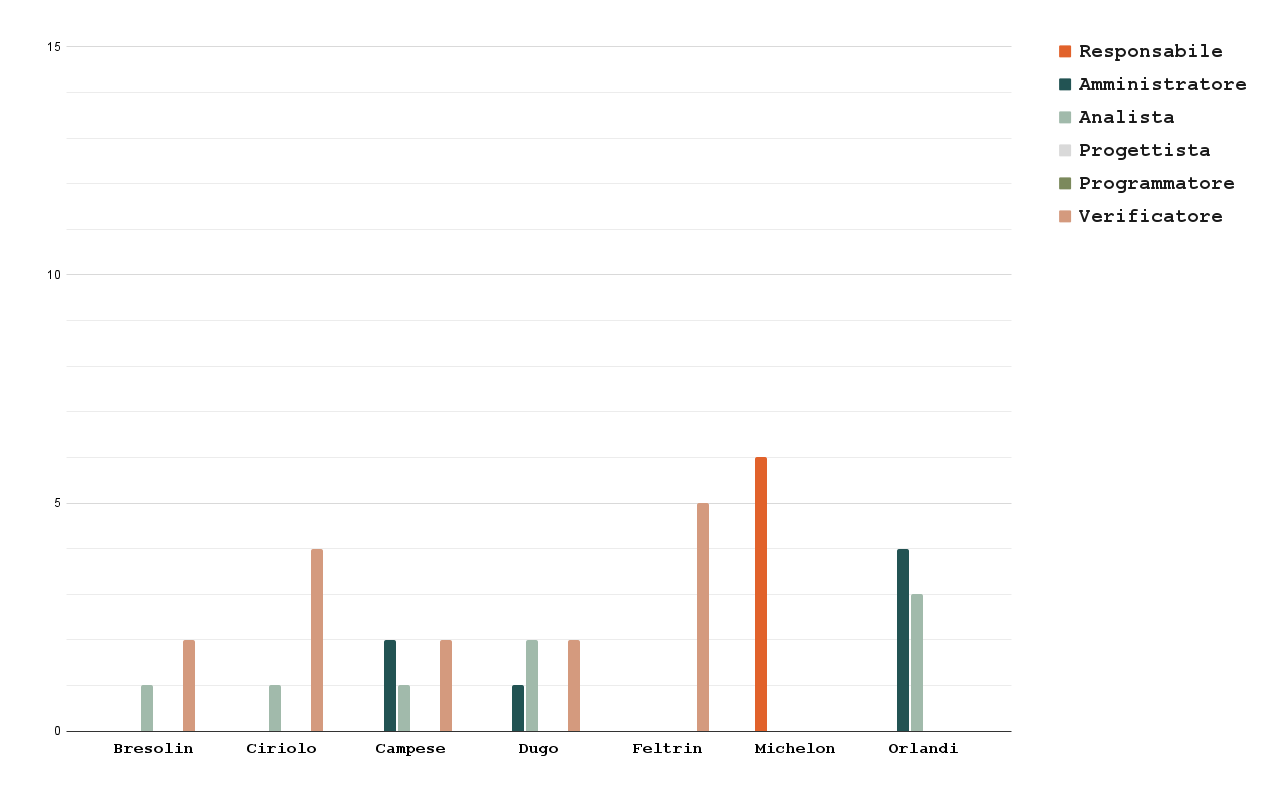
\includegraphics[width=15.5cm]{istogrammi/istogramma_5_periodo.png}
        \caption{Sprint 5 - Istogramma della ripartizione oraria dei ruoli. }
    \end{figure}

In questo incremento, il costo per ogni ruolo sarà come da tabella:
\renewcommand{\arraystretch}{1.5}
\begin{table}[H]
\centering
\begin{tabularx}{0.42\textwidth}{c|c|c}
\textbf{Ruolo} & \textbf{Ore} & \textbf{Costo}\\
\hline
\textbf{Responsabile} & 6 & 180,00\texteuro\\
\hline
\textbf{Amministratore} & 7 & 140,00\texteuro \\
\hline
\textbf{Analista} & 8 & 200,00\texteuro \\
\hline
\textbf{Progettista} & 0 & 0,00\texteuro\\
\hline
\textbf{Programmatore} & 0 & 0,00\texteuro \\ 
\hline
\textbf{Verificatore} & 15 & 225,00\texteuro \\ 
\hline
\rowcolor{primarycolor}
\textbf{Totale} & 36 & 745,00\texteuro \\
\end{tabularx}
\caption{Preventivo costi - Sprint 5}
\end{table}



La tabella è riassunta dal seguente aereogramma:
 \begin{figure}[H]
        \centering        
        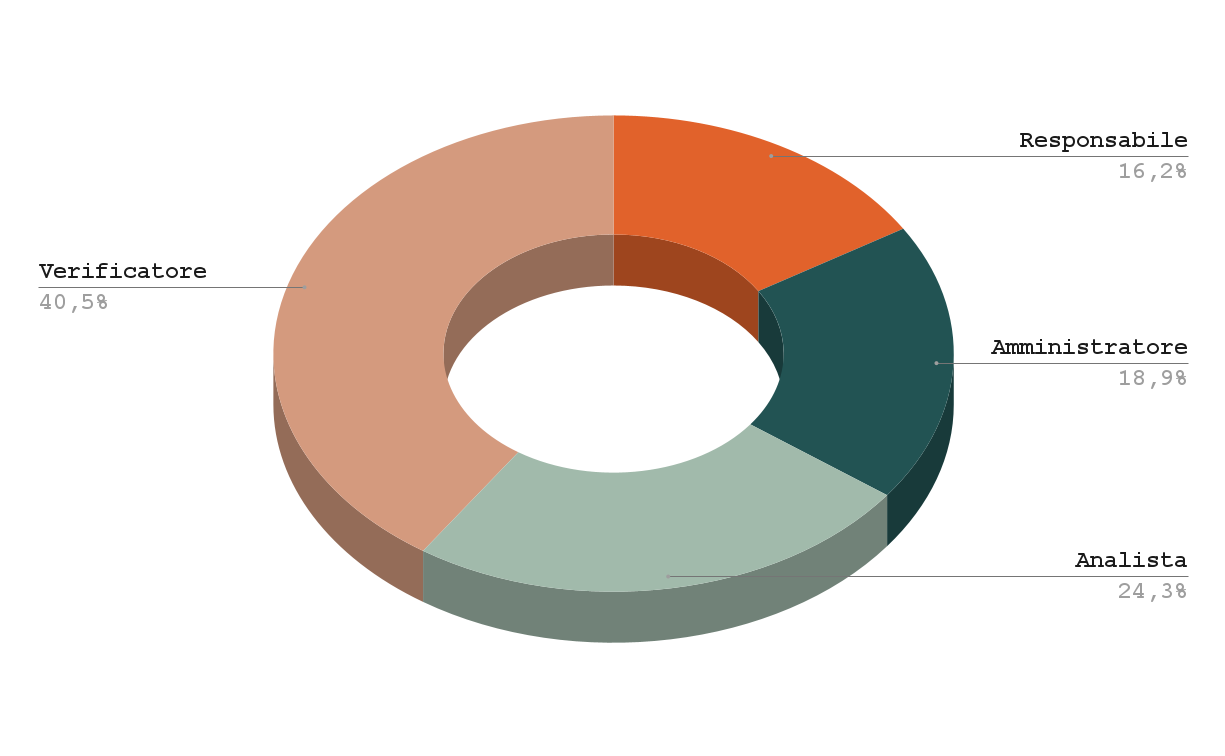
\includegraphics[width=15.5cm]{aereogrammi/areogramma_5_periodo.png}
        \caption{Sprint 5 - Areogramma della ripartizione oraria dei ruoli. }
    \end{figure}




%   PERIODO 6

\subsection{Sprint 6: da 2023-01-16 a 2024-01-30}
Di seguito, la distribuzione delle ore del sesto sprint; ogni componente del gruppo rivestirà i ruoli come segue:
\begin{table}[H]
\begin{tabularx}{\textwidth}{c|X|X|X|X|X|X|X}
        \textbf{Membri} & $\operatorname{\textbf{Re}}$ & $\mathrm{\textbf{Am}}$ & \textbf{An} & \textbf{Proj} & \textbf{Prgm} & \textbf{Ver} & \textbf{Totale} \\
        \hline Bresolin G. & 0 & \cellcolor{primarycolor}1 & 0 & 0 & 0 & 0 & 1 \\
        \hline Ciriolo I.  & 0 & \cellcolor{primarycolor}2 & 0 & 0 & 0 & 0 & 2 \\
        \hline Campese M.  & 0 & 0 & \cellcolor{primarycolor}1 & 0 & 0 & 0 & 1 \\
        \hline Dugo A.     & 0 & 0 & 0 & 0 & 0 & \cellcolor{primarycolor}1 & 1 \\
        \hline Feltrin E.  & 0 & 0 & \cellcolor{primarycolor}1 & 0 & 0 & 0 & 1 \\
        \hline Michelon R. & 0 & 0 & 0 & 0 & 0 & \cellcolor{primarycolor}2 & 2 \\
        \hline Orlandi G.  & \cellcolor{primarycolor}3 & 0 & 0 & 0 & 0 & 0 & 3 \\
        \hline
        \textbf{Totale ruolo} & 3 & 1 & 2 & 0 & 0 & 3 & 11
    \end{tabularx}
    \caption{Preventivo ore - Sprint 6}
    \end{table}

La tabella è riassunta dal seguente istogramma:
 \begin{figure}[H]
        \centering        
        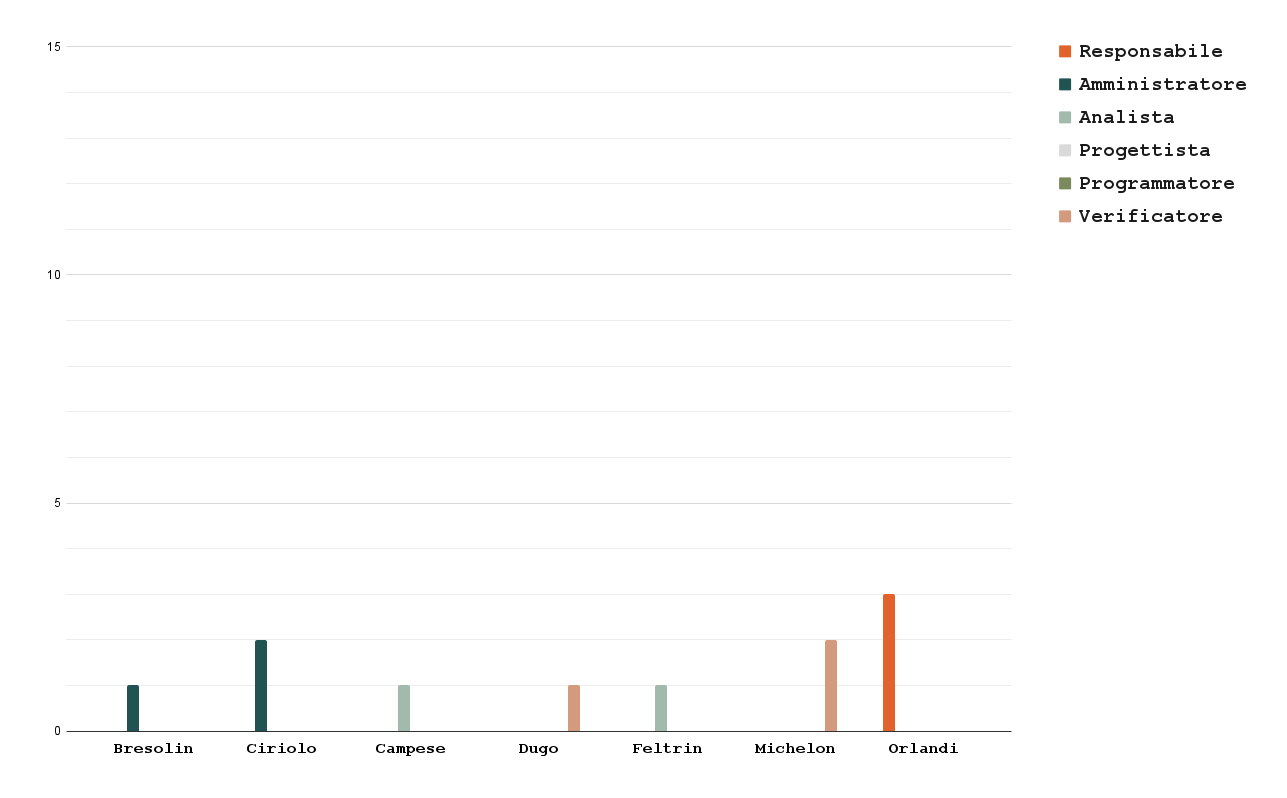
\includegraphics[width=15.5cm]{istogrammi/istogramma_6_periodo.png}
        \caption{Sprint 6 - Istogramma della ripartizione oraria dei ruoli. }
    \end{figure}


In questo incremento, il costo per ogni ruolo sarà come da tabella:
\renewcommand{\arraystretch}{1.5}
\begin{table}[H]
\centering
\begin{tabularx}{0.42\textwidth}{c|c|c}

\textbf{Ruolo} & \textbf{Ore} & \textbf{Costo}\\
\hline
\textbf{Responsabile} & 3 & 90,00\texteuro\\
\hline
\textbf{Amministratore} & 3 & 60,00\texteuro \\
\hline
\textbf{Analista} & 2 & 50,00\texteuro \\
\hline
\textbf{Progettista} & 0 & 0,00\texteuro\\
\hline
\textbf{Programmatore} & 0 & 0,00 \texteuro \\ 
\hline
\textbf{Verificatore} & 3 & 45,00\texteuro \\ 
\hline
\rowcolor{primarycolor}
\textbf{Totale} & 11 & 245,00\texteuro \\
\end{tabularx}
%}
\caption{Preventivo costi - Sprint 6}
\end{table}

La tabella è riassunta dal seguente areogramma:
 \begin{figure}[H]
        \centering        
        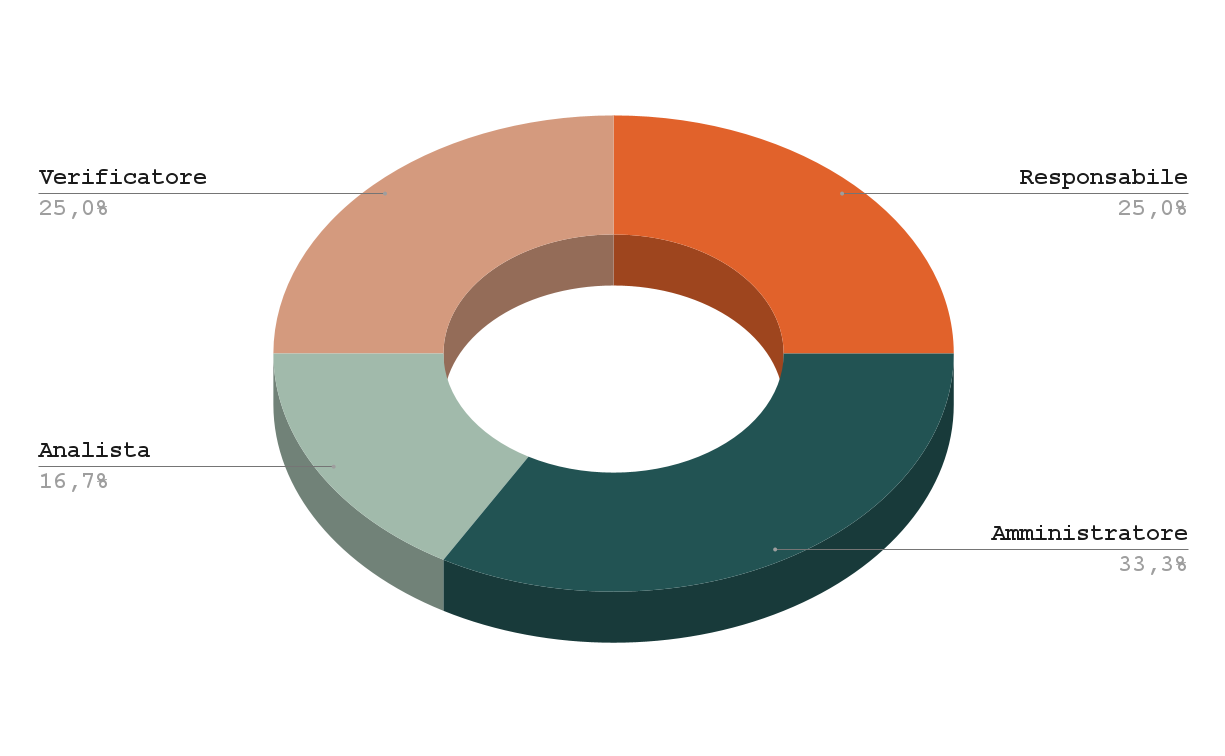
\includegraphics[width=15.5cm]{aereogrammi/areogramma_6_periodo.png}
        \caption{Sprint 6 - Areogramma della ripartizione oraria dei ruoli. }
    \end{figure}





%   PERIODO 7
\subsection{Sprint 7: da 2024-01-30 a 2024-02-13}
Di seguito, la distribuzione delle ore del settimo sprint; ogni componente del gruppo rivestirà i ruoli come segue:
\begin{table}[H]
\begin{tabularx}{\textwidth}{c|X|X|X|X|X|X|X}
    \textbf{Membri} & $\operatorname{\textbf{Re}}$ & $\mathrm{\textbf{Am}}$ & \textbf{An} & \textbf{Proj} & \textbf{Prgm} & \textbf{Ver} & \textbf{Totale} \\
        \hline Bresolin G. & \cellcolor{primarycolor}4 & 0 & 0 & 1 & 0 & 0 & 5 \\
        \hline Ciriolo I.  & 0 & 1 & 0 & \cellcolor{primarycolor}4 & 0 & 0 & 5 \\
        \hline Campese M.  & 0 & 0 & 0 & \cellcolor{primarycolor}3 & 0 & 0 & 3 \\
        \hline Dugo A.     & 0 & 0 & \cellcolor{primarycolor}2 & 2 & 0 & 0 & 4 \\
        \hline Feltrin E.  & 0 & 0 & 0 & 1 & 0 & \cellcolor{primarycolor}2 & 3 \\
        \hline Michelon R. & 0 & \cellcolor{primarycolor}2 & 0 & 1 & 0 & 1 & 4 \\
        \hline Orlandi G.  & 0 & 0 & 0 & 1 & \cellcolor{primarycolor}4 & 0 & 5 \\
        \hline
        \textbf{Totale ruolo} & 4 & 3 & 2 & 13 & 4 & 3 & 29 
    \end{tabularx}
    \caption{Preventivo ore - Sprint 7}
    \end{table}

La tabella è riassunta dal seguente istogramma:
 \begin{figure}[H]
        \centering        
        \includegraphics[width=15.5cm]{istogrammi/istogramma_7_periodo.png}
        \caption{Sprint 7- Istogramma della ripartizione oraria dei ruoli. }
    \end{figure}

In questo incremento, il costo per ogni ruolo sarà come da tabella:
\renewcommand{\arraystretch}{1.5}
\begin{table}[H]
\centering
\begin{tabularx}{0.42\textwidth}{c|c|c}

\textbf{Ruolo} & \textbf{Ore} & \textbf{Costo}\\
\hline
\textbf{Responsabile} & 4 & 120,00\texteuro\\
\hline
\textbf{Amministratore} & 3 & 60,00\texteuro \\
\hline
\textbf{Analista} & 2 & 50,00\texteuro \\
\hline
\textbf{Progettista} & 13 & 325,00\texteuro\\
\hline
\textbf{Programmatore} & 4 & 60,00 \texteuro \\ 
\hline
\textbf{Verificatore} & 4 & 60,00\texteuro \\ 
\hline
\rowcolor{primarycolor}
\textbf{Totale} & 29 & 675,00\texteuro \\
\end{tabularx}
%}
\caption{Preventivo costi - Sprint 7}
\end{table}

La tabella è riassunta dal seguente areogramma:
 \begin{figure}[H]
        \centering        
        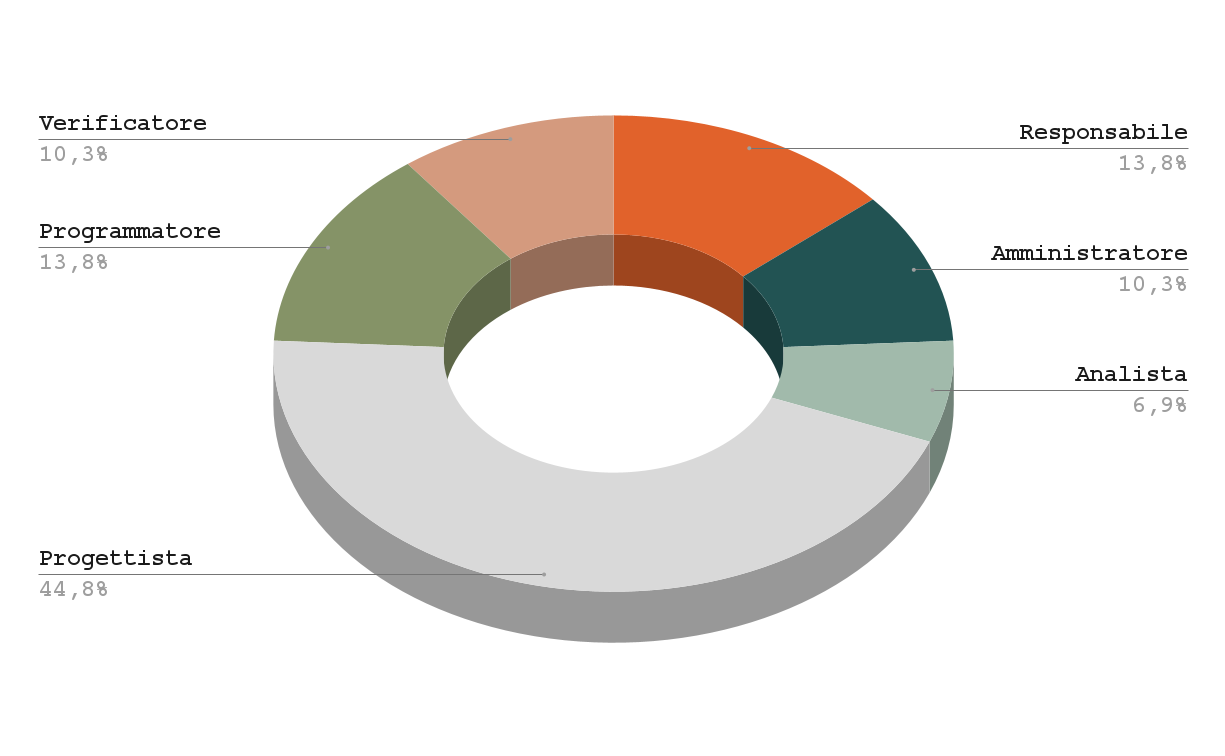
\includegraphics[width=15.5cm]{aereogrammi/areogramma_7_periodo.png}
        \caption{Sprint 7 - Areogramma della ripartizione oraria dei ruoli. }
    \end{figure}


%   PERIODO 8
\subsection{Sprint 8: da 2024-02-13 a 2024-02-27}
\subsubsection{Preventivo delle ore e dei costi}
Di seguito, la distribuzione delle ore dell'ottavo sprint; ogni componente del gruppo rivestirà i ruoli come segue:
\begin{table}[H]
\begin{tabularx}{\textwidth}{c|X|X|X|X|X|X|X}
    \textbf{Membri} & $\operatorname{\textbf{Re}}$ & $\mathrm{\textbf{Am}}$ & \textbf{An} & \textbf{Proj} & \textbf{Prgm} & \textbf{Ver} & \textbf{Totale} \\
        \hline Bresolin G. & 0 & \cellcolor{primarycolor}2 & 0 & 8 & 5 & 0 & 15 \\
        \hline Ciriolo I.  & \cellcolor{primarycolor}4 & 0 & 0 & 6 & 0 & 5 & 15 \\
        \hline Campese M.  & 0 & 0 & 1 & 7 & \cellcolor{primarycolor}9 & 0 & 17 \\
        \hline Dugo A.     & 0 & 1 & 0 & \cellcolor{primarycolor}8 & 0 & 3 & 12 \\
        \hline Feltrin E.  & 0 & 0 & 1 & 4 & \cellcolor{primarycolor}10 & 0 & 15 \\
        \hline Michelon R. & 0 & 0 & 0 & 5 & 5 & \cellcolor{primarycolor}4 & 14 \\
        \hline Orlandi G.  & 0 & 0 & 0 & \cellcolor{primarycolor}5 & 4 & 0 & 10 \\
        \hline
        \textbf{Totale ruolo} & 4 & 4 & 2 & 43 & 33 & 12 & 98 
    \end{tabularx}
    \caption{Preventivo ore - Sprint 8}
    \end{table}

La tabella è riassunta dal seguente istogramma:
 \begin{figure}[H]
        \centering        
        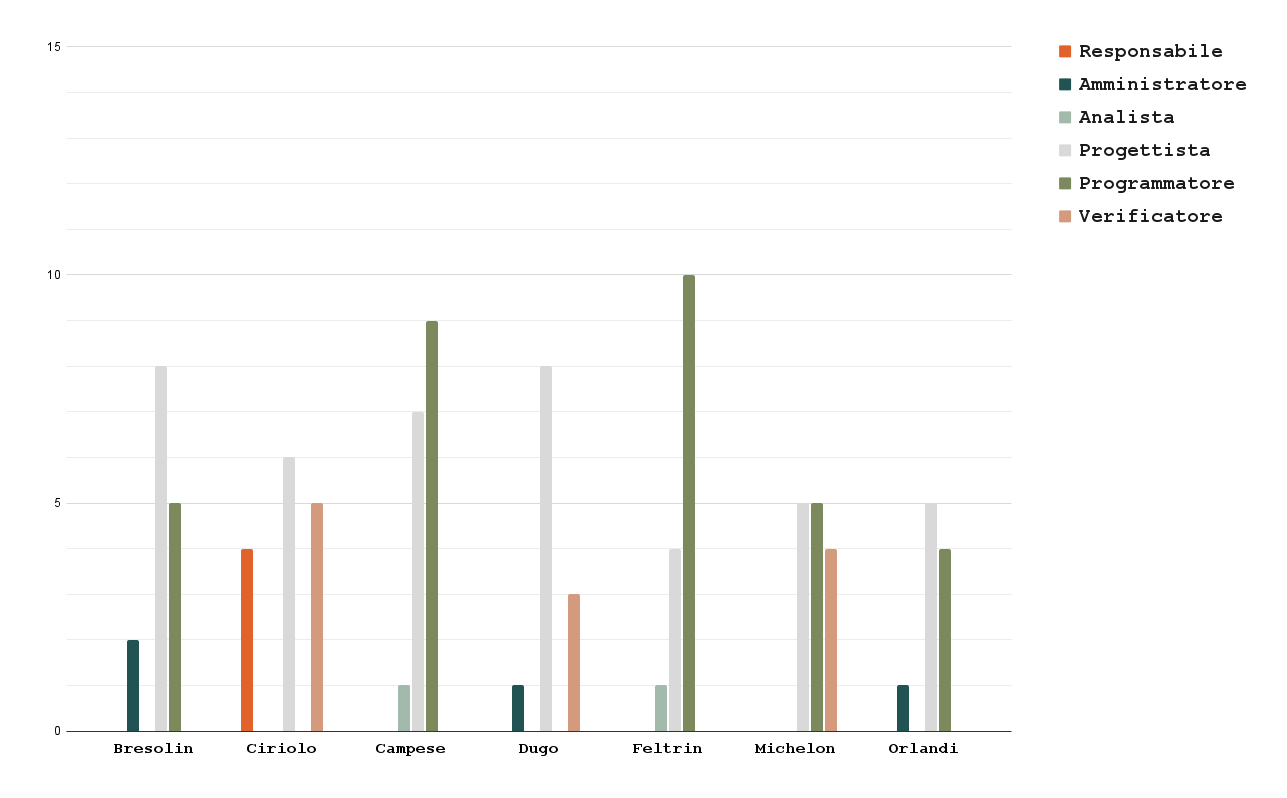
\includegraphics[width=15.5cm]{istogrammi/istogramma_8_periodo.png}
        \caption{Sprint 8- Istogramma della ripartizione oraria dei ruoli. }
    \end{figure}

In questo incremento, il costo per ogni ruolo sarà come da tabella:
\renewcommand{\arraystretch}{1.5}
\begin{table}[H]
\centering
\begin{tabularx}{0.42\textwidth}{c|c|c}

\textbf{Ruolo} & \textbf{Ore} & \textbf{Costo}\\
\hline
\textbf{Responsabile} & 4 & 120,00\texteuro\\
\hline
\textbf{Amministratore} & 4 & 80,00\texteuro \\
\hline
\textbf{Analista} & 2 & 50,00\texteuro \\
\hline
\textbf{Progettista} & 43 & 1075,00\texteuro\\
\hline
\textbf{Programmatore} & 33 & 495,00 \texteuro \\ 
\hline
\textbf{Verificatore} & 12 & 180,00\texteuro \\ 
\hline
\rowcolor{primarycolor}
\textbf{Totale} & 98 & 2000,00\texteuro \\
\end{tabularx}
%}
\caption{Preventivo costi - Sprint 8}
\end{table}

La tabella è riassunta dal seguente areogramma:
 \begin{figure}[H]
        \centering        
        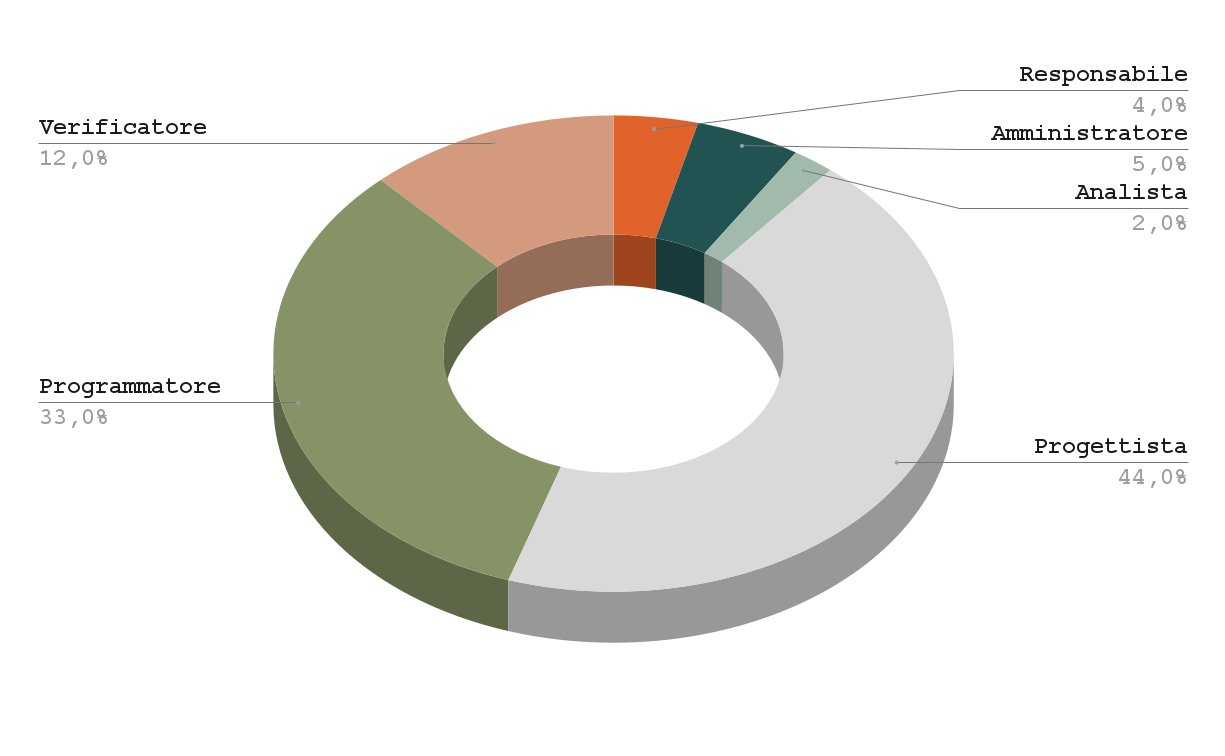
\includegraphics[width=15.5cm]{aereogrammi/areogramma_8_periodo.png}
        \caption{Sprint 8 - Areogramma della ripartizione oraria dei ruoli. }
    \end{figure}
\subsubsection{Previsione occorrenze eventuali rischi:}
\begin{itemize}
    \item \textbf{RP.1}: non disponibilità di alcuni membri del gruppo per cause/impegni personali;
    \item \textbf{RT.1}: scarsa esperienza nella progettazione logica e di dettaglio.
\end{itemize}

%   PERIODO 9
\subsection{Sprint 9: da 2024-02-27 a 2024-03-12}

\subsubsection{Preventivo delle ore e dei costi}
Di seguito, la distribuzione delle ore del nono sprint; ogni componente del gruppo rivestirà i ruoli come segue:
\begin{table}[H]
\begin{tabularx}{\textwidth}{c|X|X|X|X|X|X|X}
    \textbf{Membri} & $\operatorname{\textbf{Re}}$ & $\mathrm{\textbf{Am}}$ & \textbf{An} & \textbf{Proj} & \textbf{Prgm} & \textbf{Ver} & \textbf{Totale} \\
        \hline Bresolin G. & 0 & 0 & 1 & 1 & 9 & \cellcolor{primarycolor}10 & 21 \\
        \hline Ciriolo I.  & 0 & 0 & 0 & 2 & \cellcolor{primarycolor}11 & 0 & 13 \\
        \hline Campese M.  & 0 & 4 & 0 & 2 & \cellcolor{primarycolor}8 & 5 & 19 \\
        \hline Dugo A.     & 0 & 0 & 0 & 0 & 9 & \cellcolor{primarycolor}9 & 18 \\
        \hline Feltrin E.  & 0 & 0 & 0 & \cellcolor{primarycolor}7 & 7 & 4 & 18 \\
        \hline Michelon R. & 0 & 0 & 0 & 3 & \cellcolor{primarycolor}11 & 0 & 14 \\
        \hline Orlandi G.  & \cellcolor{primarycolor}6 & 0 & 0 & 5 & 6 & 1 & 18 \\
        \hline
        \textbf{Totale ruolo} & 6 & 4 & 1 & 20 & 61 & 29 & 121 
    \end{tabularx}
    \caption{Preventivo ore - Sprint 9}
    \end{table}

La tabella è riassunta dal seguente istogramma:
 \begin{figure}[H]
        \centering        
        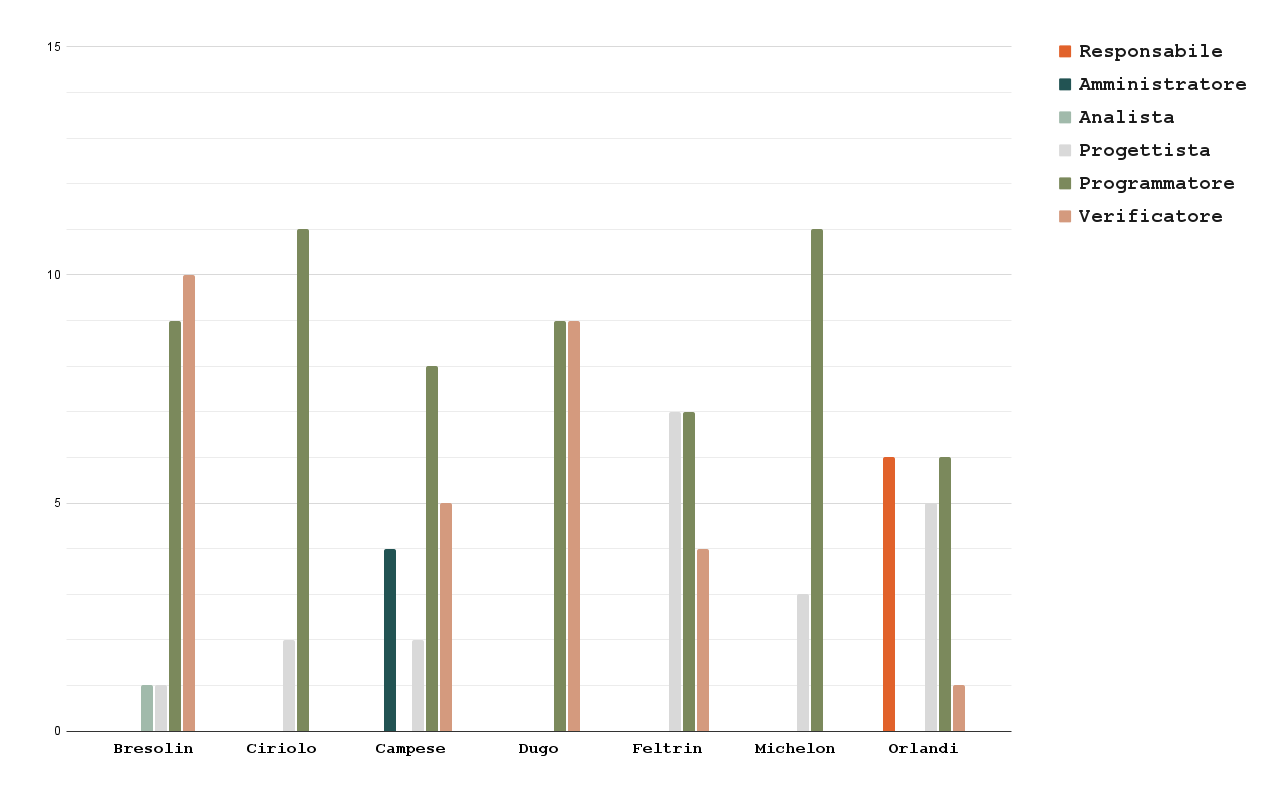
\includegraphics[width=15.5cm]{istogrammi/istogramma_9_periodo.png}
        \caption{Sprint 9- Istogramma della ripartizione oraria dei ruoli. }
    \end{figure}

In questo incremento, il costo per ogni ruolo sarà come da tabella:
\renewcommand{\arraystretch}{1.5}
\begin{table}[H]
\centering
\begin{tabularx}{0.42\textwidth}{c|c|c}

\textbf{Ruolo} & \textbf{Ore} & \textbf{Costo}\\
\hline
\textbf{Responsabile} & 6 & 180,00\texteuro\\
\hline
\textbf{Amministratore} & 4 & 80,00\texteuro \\
\hline
\textbf{Analista} & 1 & 25,00\texteuro \\
\hline
\textbf{Progettista} & 20 & 500,00\texteuro\\
\hline
\textbf{Programmatore} & 61 & 915,00 \texteuro \\ 
\hline
\textbf{Verificatore} & 29 & 435,00\texteuro \\ 
\hline
\rowcolor{primarycolor}
\textbf{Totale} & 121 & 2135,00\texteuro \\
\end{tabularx}
%}
\caption{Preventivo costi - Sprint 9}
\end{table}

La tabella è riassunta dal seguente areogramma:
 \begin{figure}[H]
        \centering        
        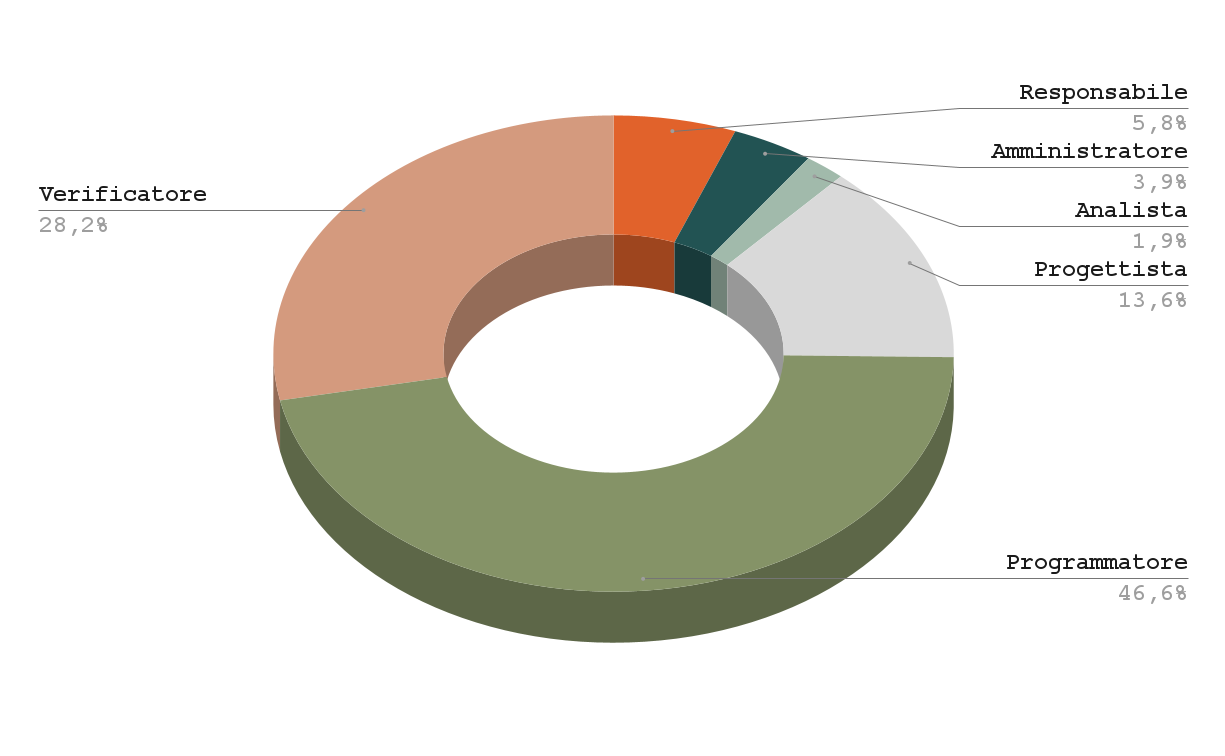
\includegraphics[width=15.5cm]{aereogrammi/areogramma_9_periodo.png}
        \caption{Sprint 9 - Areogramma della ripartizione oraria dei ruoli. }
    \end{figure}

    \subsubsection{Previsione occorrenze eventuali rischi:}
    \begin{itemize}
        \item \textbf{RT.1}: scarsa esperienza nell'uso delle tecnologie per le attività di codifica e di testing.
    \end{itemize}


%   PERIODO 10
\subsection{Sprint 10: da 2024-03-12 a 2024-03-26}

\subsubsection{Preventivo delle ore e dei costi}
Di seguito, la distribuzione delle ore del decimo sprint; ogni componente del gruppo rivestirà i ruoli come segue:
\begin{table}[H]
\begin{tabularx}{\textwidth}{c|X|X|X|X|X|X|X}
    \textbf{Membri} & $\operatorname{\textbf{Re}}$ & $\mathrm{\textbf{Am}}$ & \textbf{An} & \textbf{Proj} & \textbf{Prgm} & \textbf{Ver} & \textbf{Totale} \\
        \hline Bresolin G. & \cellcolor{primarycolor}5 & 0 & 0 & 0 & 9 & 0 & 14 \\
        \hline Ciriolo I.  & 0 & 0 & 1 & 0 & \cellcolor{primarycolor}12 & 3 & 16 \\
        \hline Campese M.  & 0 & 0 & 1 & 2 & \cellcolor{primarycolor}12 & 1 & 16 \\
        \hline Dugo A.     & 0 & 0 & 0 & 0 & \cellcolor{primarycolor}9 & 4 & 13 \\
        \hline Feltrin E.  & 0 & 4 & 0 & 1 & 7 & \cellcolor{primarycolor}5 & 17 \\
        \hline Michelon R. & 0 & 0 & 0 & 0 & 6 & \cellcolor{primarycolor}7 & 13 \\
        \hline Orlandi G.  & 0 & 0 & 0 & 0 & 10 & \cellcolor{primarycolor}10 & 20 \\
        \hline
        \textbf{Totale ruolo} & 5 & 4 & 2 & 3 & 65 & 30 & 109 
    \end{tabularx}
    \caption{Preventivo ore - Sprint 10}
    \end{table}

La tabella è riassunta dal seguente istogramma:
 \begin{figure}[H]
        \centering        
        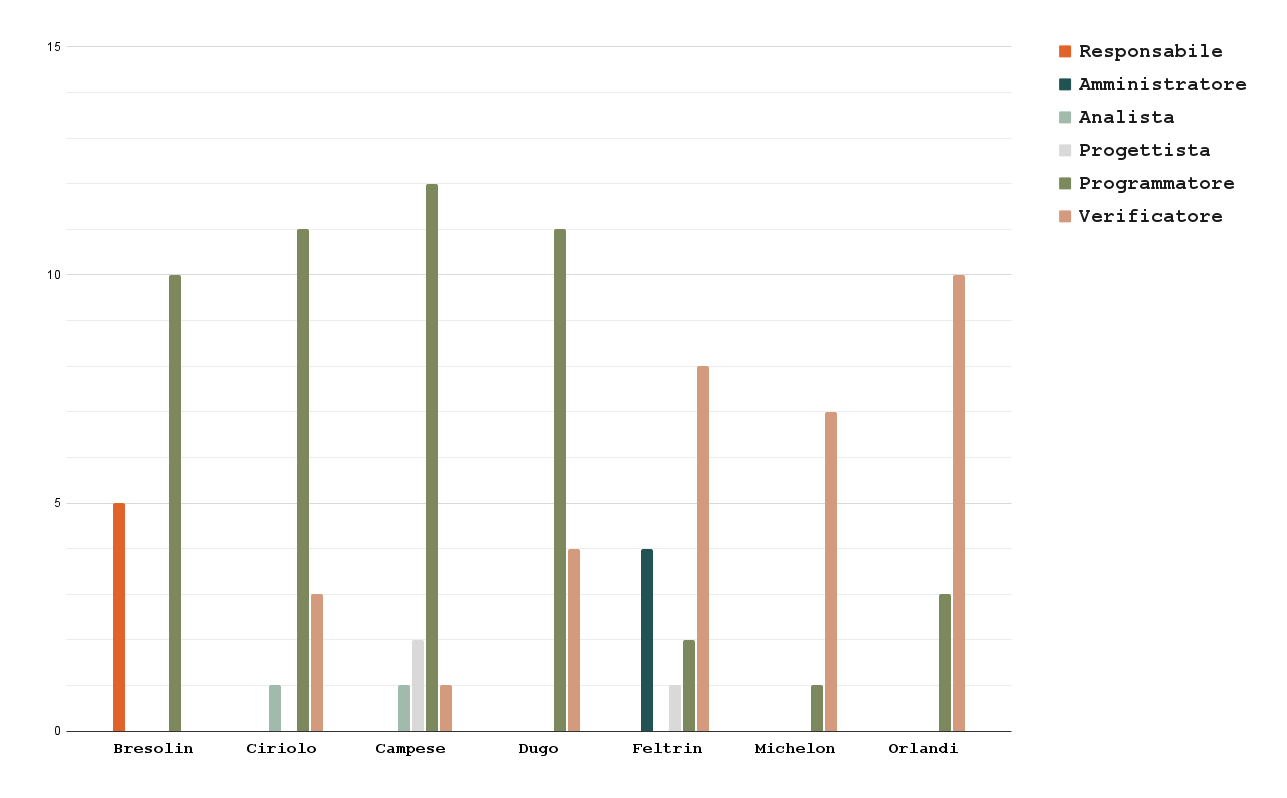
\includegraphics[width=15.5cm]{istogrammi/istogramma_10_periodo.png}
        \caption{Sprint 10 - Istogramma della ripartizione oraria dei ruoli. }
    \end{figure}

In questo incremento, il costo per ogni ruolo sarà come da tabella:
\renewcommand{\arraystretch}{1.5}
\begin{table}[H]
\centering
\begin{tabularx}{0.42\textwidth}{c|c|c}

\textbf{Ruolo} & \textbf{Ore} & \textbf{Costo}\\
\hline
\textbf{Responsabile} & 5 & 150,00\texteuro\\
\hline
\textbf{Amministratore} & 4 & 80,00\texteuro \\
\hline
\textbf{Analista} & 2 & 50,00\texteuro \\
\hline
\textbf{Progettista} & 3 & 75,00\texteuro\\
\hline
\textbf{Programmatore} & 65 & 675,00 \texteuro \\ 
\hline
\textbf{Verificatore} & 30 & 450,00\texteuro \\ 
\hline
\rowcolor{primarycolor}
\textbf{Totale} & 109 & 1780,00\texteuro \\
\end{tabularx}
%}
\caption{Preventivo costi - Sprint 10}
\end{table}

La tabella è riassunta dal seguente areogramma:
 \begin{figure}[H]
        \centering        
        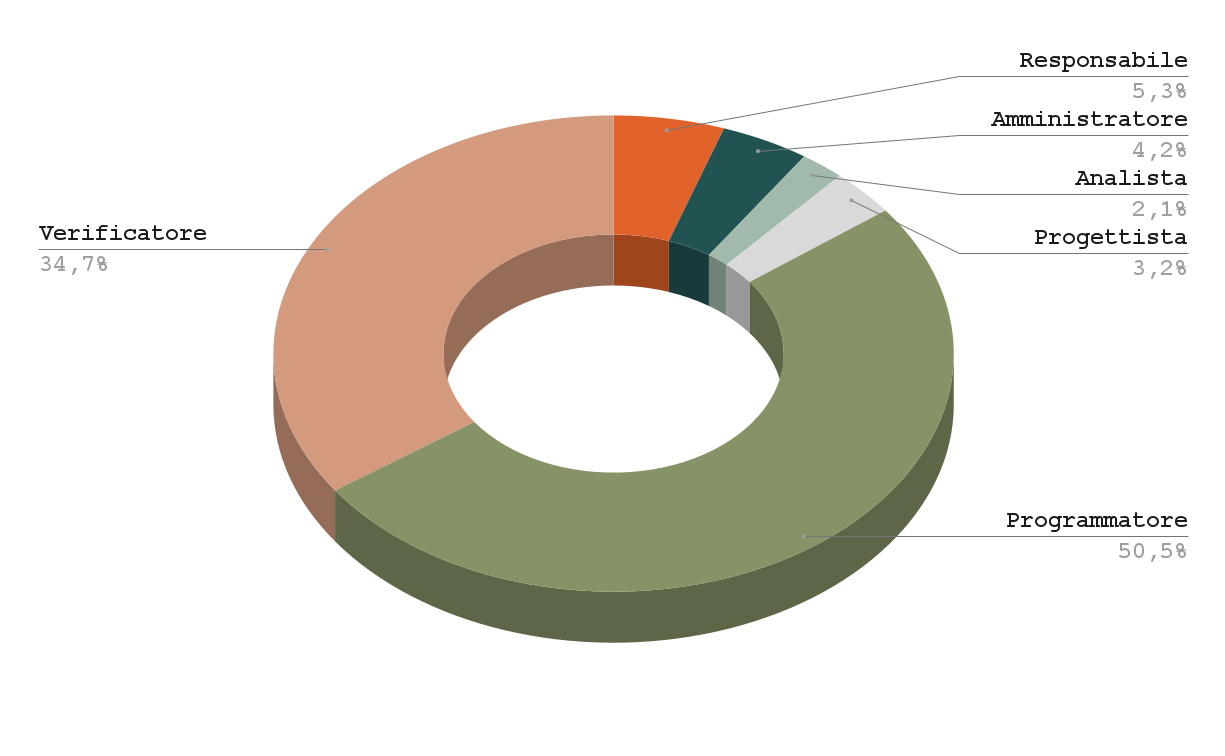
\includegraphics[width=15.5cm]{aereogrammi/areogramma_10_periodo.png}
        \caption{Sprint 10 - Areogramma della ripartizione oraria dei ruoli. }
    \end{figure}
    

    \subsubsection{Previsione occorrenze eventuali rischi:}
\begin{itemize}
    \item \textbf{RT.1}: scarsa esperienza nell'uso delle tecnologie per le attività di codifica e di testing.
\end{itemize}

% Periodo 11

\subsection{Sprint 11: da 2024-03-26 a 2024-04-08}

\subsubsection{Preventivo delle ore e dei costi}
Di seguito, la distribuzione delle ore del undicesimo sprint; ogni componente del gruppo rivestirà i ruoli come segue:
\begin{table}[H]
\begin{tabularx}{\textwidth}{c|X|X|X|X|X|X|X}
\textbf{Membri} & $\operatorname{\textbf{Re}}$ & $\mathrm{\textbf{Am}}$ & \textbf{An} & \textbf{Proj} & \textbf{Prgm} & \textbf{Ver} & \textbf{Totale} \\
\hline Bresolin & 0 & 0 & 0 & 0 & \cellcolor{primarycolor}6 & 5 & 11 \\
\hline Ciriolo & 0 & \cellcolor{primarycolor}4 & 0 & 0 & 4 & 2 & 10 \\
\hline Campese & 0 & 0 & 0 & 0 & \cellcolor{primarycolor}6 & 3 & 9 \\
\hline Dugo & \cellcolor{primarycolor}5 & 0 & 0 & 0 & 1 & 3 & 9 \\
\hline Feltrin & 0 & 0 & 0 & 0 & 2 & \cellcolor{primarycolor}9 & 11 \\
\hline Michelon & 0 & 1 & 1 & 0 & 0 & \cellcolor{primarycolor}9 & 11 \\
\hline Orlandi & 0 & 4 & 1 & 0 & \cellcolor{primarycolor}3 & 3 & 11 \\
\hline
\textbf{Totale ruolo} & 5 & 9 & 2 & 0 & 22 & 34 & 72
\end{tabularx}
\caption{Preventivo ore - Sprint 11}
\end{table}

La tabella è riassunta dal seguente istogramma:
 \begin{figure}[H]
        \centering        
        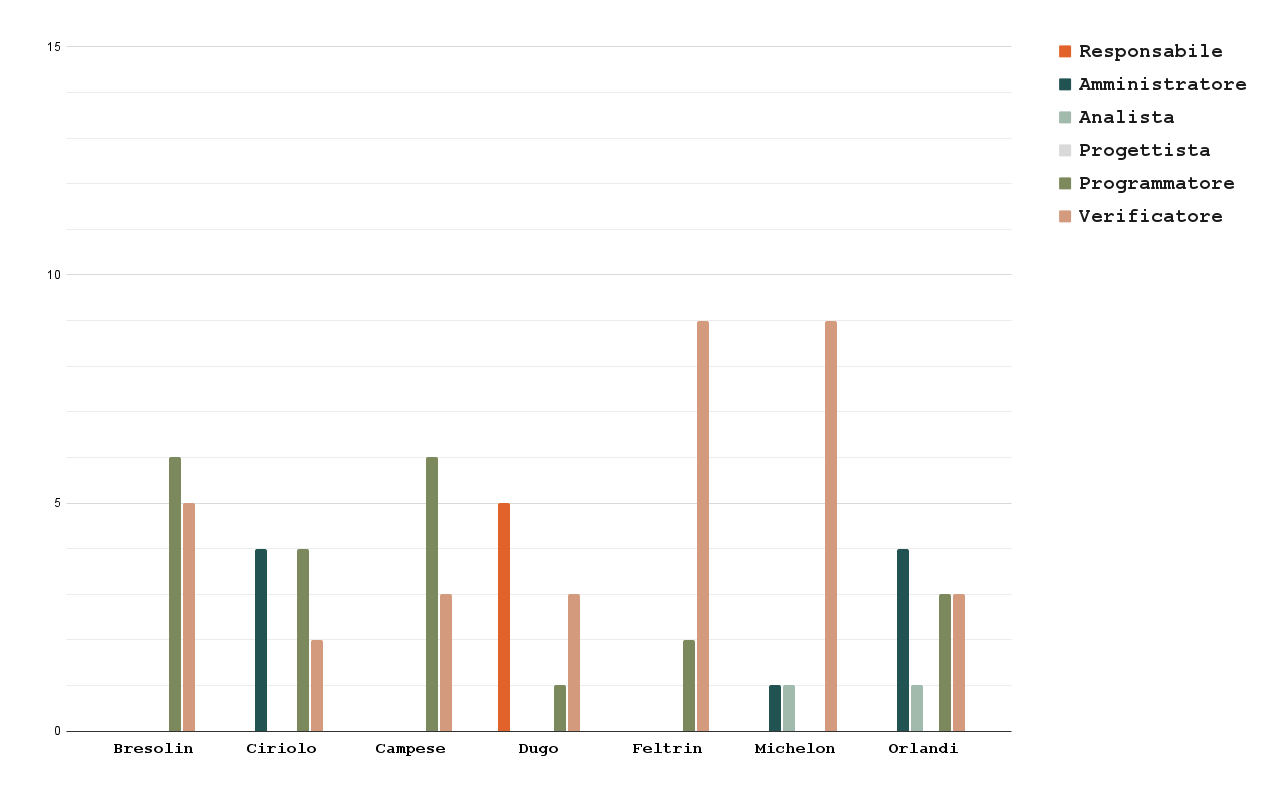
\includegraphics[width=15.5cm]{istogrammi/istogramma_11_periodo.png}
        \caption{Sprint 11- Istogramma della ripartizione oraria dei ruoli. }
    \end{figure}

In questo incremento, il costo per ogni ruolo sarà come da tabella:
\renewcommand{\arraystretch}{1.5}
\begin{table}[H]
\centering
\begin{tabularx}{0.42\textwidth}{c|c|c}

\textbf{Ruolo} & \textbf{Ore} & \textbf{Costo}\\
\hline
\textbf{Responsabile} & 5 & 150,00\texteuro\\
\hline
\textbf{Amministratore} & 9 & 180,00\texteuro \\
\hline
\textbf{Analista} & 2 & 50,00\texteuro \\
\hline
\textbf{Progettista} & 0 & 0,00\texteuro\\
\hline
\textbf{Programmatore} & 22 & 330,00 \texteuro \\ 
\hline
\textbf{Verificatore} & 34 & 510,00\texteuro \\ 
\hline
\rowcolor{primarycolor}
\textbf{Totale} & 72 & 1120,00\texteuro \\
\end{tabularx}
%}
\caption{Preventivo costi - Sprint 11}
\end{table}

La tabella è riassunta dal seguente areogramma:
 \begin{figure}[H]
        \centering        
        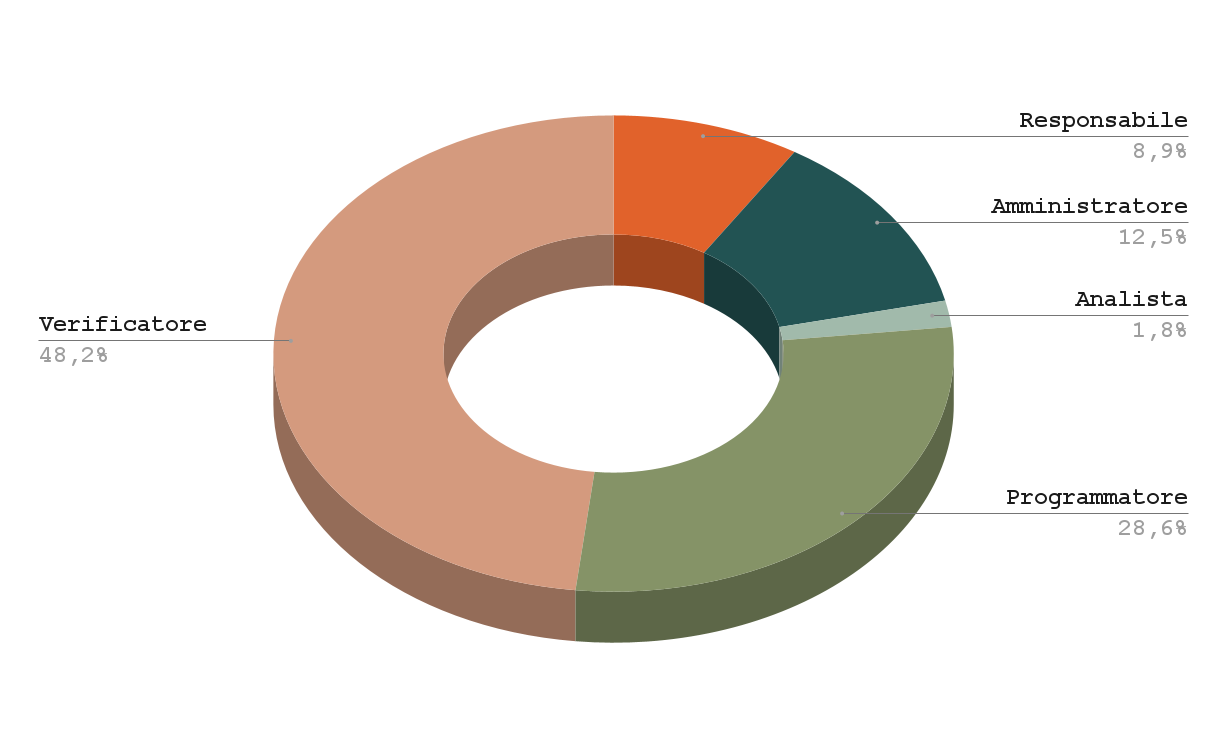
\includegraphics[width=15.5cm]{aereogrammi/areogramma_11_periodo.png}
        \caption{Sprint 11 - Areogramma della ripartizione oraria dei ruoli. }
    \end{figure}

    \subsubsection{Previsione occorrenze eventuali rischi:}
    \begin{itemize}
        \item \textbf{RP.1}: Impegni universitari per alcuni membri del gruppo;
        \item \textbf{RT.1}: Scarsa esperienza nell'uso delle tecnologie per le attività di codifica e di testing.
    \end{itemize}

\newpage

%   CONSUNTIVO

\section{Consuntivo}

% PERIODO 1 CONSUNTIVO
\subsection{Sprint 1: da 2023-11-07 a 2023-11-21}
Di seguito, la distribuzione delle ore del primo sprint; ogni componente del gruppo ha rivestito i ruoli come segue:
\begin{table}[H]
\begin{tabularx}{\textwidth}{c|X|X|X|X|X|X|X}
        \textbf{Membri} & $\operatorname{\textbf{Re}}$ & $\mathrm{\textbf{Am}}$ & \textbf{An} & \textbf{Proj} & \textbf{Prgm} & \textbf{Ver} & \textbf{Totale} \\
        \hline Bresolin G. & 0 & 5 & 0 & 0 & 0 & 0 & 5 \\
        \hline Ciriolo I.  & 0 & 0 & 7 & 0 & 0 & 1 & 8 \\
        \hline Campese M.  & 0 & 0 & 2 & 0 & 0 & 7 & 9 \\
        \hline Dugo A.     & 0 & 5 & 0 & 0 & 0 & 0 & 5 \\
        \hline Feltrin E.  & 7 & 1 & 0 & 0 & 0 & 0 & 8 \\
        \hline Michelon R. & 0 & 6 & 0 & 0 & 0 & 0 & 6 \\
        \hline Orlandi G.  & 0 & 0 & 3 & 0 & 0 & 1 & 4 \\
        \hline
        \textbf{Totale ruolo} & 7 & 17 & 12 & 0 & 0 & 9 & 45 
    \end{tabularx}
    \caption{Consuntivo ore - Sprint 1}
    \end{table}


\begin{table}[H]
\begin{tabularx}{\textwidth}{c|X|X|X|X|X|X}
        \textbf{Ruolo} & \textbf{Ore preventivo} & \textbf{Ore consuntivo} & \textbf{Delta ore} & \textbf{Costo preventivo} & \textbf{Costo consuntivo} & \textbf{Delta costo} \\
        \hline
        \textbf{RES} & 8 & 7 & 1 & 240,00\texteuro & € 210,00\texteuro & € 30,00\texteuro \\
        \hline
        \textbf{AMM} & 15 & 17 & -2 & 300,00\texteuro & 340,00\texteuro & -€ 40,00\texteuro \\
        \hline
        \textbf{AN} & 11 & 12 & -1 & 275,00\texteuro & 300,00\texteuro & -€ 25,00\texteuro \\
        \hline
        \textbf{PROJ} & 0 & 0 & 0 & 0,00\texteuro & 0,00\texteuro & € 0,00\texteuro \\
        \hline
        \textbf{PROG} & 0 & 0 & 0 & 0,00\texteuro & € 0,00 & € 0,00\texteuro \\
        \hline
        \textbf{VER} & 10 & 9 & 1 & 150,00\texteuro & € 135,00 & € 15,00\texteuro \\
        \hline
        \rowcolor{primarycolor}
        \textbf{TOT} & 44 & 45 & -1 & 965,00\texteuro & 985,00\texteuro & -20,00\texteuro
    \end{tabularx}
    \caption{Consuntivo costi - Sprint 1}
\end{table}

\subsubsection{Revisione}
Il team nel primo sprint ha svolto le seguenti attività:
\begin{itemize}
    \item Stilato Piano di progetto;
    \item Effettuata la migrazione verso l'\textit{ITS\pg} \textit{Jira\pg} di \textit{Atlassian};
    \item Automatizzato versionamento repository;
    \item Prima stesura Analisi dei requisiti;
    \item Stilato verbali relativi allo sprint.
\end{itemize}
\subsubsection{Retrospettiva}
\begin{itemize}
\item Il consuntivo di periodo possiede delle discrepanze rispetto al preventivo stilato. Questo è dovuto alla sottostima delle 
tempistiche per alcune attività onerose che si sono rivelate più importanti dal punto di vista delle ore necessarie;
\item A seguito di incomprensioni tra le componenti del gruppo, sono state stilate in maniera non sufficiente alcune sezioni del 
Piano di Qualifica; questo ha comportato un ritardo e un aggiornamento della pianificazione che tenesse conto della nuova stesura del documento;
\item La parametrizzazione dei documenti realizzata a fine sprint, in particolar modo per la produzione dei verbali interni ed esterni, ha riscontrato un notevole apprezzamento
da parte del team, aumentando l'\textit{efficienza\pg} dal punto di vista della risorsa tempo, semplificando l'inserimento delle informazioni richieste, notando
in fase di revisione una riduzione consistente degli errori di formattazione, di collocazione e di omissione di informazione;
\item L'automazione del versionamento tramite \textit{script\pg} e \textit{GitHub Actions\pg}, seppur sia stata costosa in termine di risorse impiegate,
risulta essere efficace, rimuovendo tutti gli errori di calcolo che erano prima causati dai membri del team, i quali ora non devono più occuparsi di tale compito;
\item La migrazione verso il nuovo ITS \textit{Jira}, seppur sia in utilizzo solamente dal presente sprint, ha fatto emergere un feedback migliore rispetto all'ITS 
offerto da \textit{GitHub}, grazie alla maggior integrazione di strumenti in linea con il metodo Agile. Inoltre, è risultato evidente al team che \textit{Jira} è stato concepito 
con l'obiettivo primario di fungere da ITS, presentando funzionalità che agevolano la gestione dei task.
\end{itemize}
%PERIODO 2 CONSUNTIVO
\subsection{Sprint 2: da 2023-11-21 a 2023-12-05}
Di seguito, la distribuzione delle ore del secondo sprint; ogni componente del gruppo ha rivestito i ruoli come segue:
\begin{table}[H]
\begin{tabularx}{\textwidth}{c|X|X|X|X|X|X|X}
        \textbf{Membri} & $\operatorname{\textbf{Re}}$ & $\mathrm{\textbf{Am}}$ & \textbf{An} & \textbf{Proj} & \textbf{Prgm} & \textbf{Ver} & \textbf{Totale} \\
        \hline Bresolin G. & 0 & 1 & 7 & 0 & 0 & 0 & 8 \\
        \hline Ciriolo I.  & 7 & 0 & 0 & 0 & 0 & 1 & 8 \\
        \hline Campese M.  & 0 & 4 & 2 & 0 & 0 & 1,5 & 7,5 \\
        \hline Dugo A.     & 0 & 0 & 2 & 2 & 9 & 0 & 13 \\
        \hline Feltrin E.  & 0 & 0 & 0 & 0 & 11 & 0 & 11 \\
        \hline Michelon R. & 0 & 0 & 2 & 1 & 13 & 0 & 16 \\
        \hline Orlandi G.  & 0 & 0 & 0 & 0 & 0 & 7 & 7 \\
        \hline
        \textbf{Totale ruolo} & 7 & 5 & 13 & 3 & 33 & 9,5 & 70,5 
    \end{tabularx}
    \caption{Consuntivo ore - Sprint 2}
    \end{table}
 
\begin{table}[H]
\begin{tabularx}{\textwidth}{c|X|X|X|X|X|X}
        \textbf{Ruolo} & \textbf{Ore preventivo} & \textbf{Ore consuntivo} & \textbf{Delta orario} & \textbf{Costo preventivo} & \textbf{Costo consuntivo} & \textbf{Delta costo} \\
        \hline
        \textbf{RES} & 7 & 7 & 0 & 210,00\texteuro & 210,00\texteuro &  0,00\texteuro \\
        \hline
        \textbf{AMM} & 6 & 5 & 1 & 120,00\texteuro & 100,00\texteuro & 20,00\texteuro \\
        \hline
        \textbf{AN} & 12 & 13 & -1 & 300,00\texteuro & 325,00\texteuro & -25,00\texteuro \\
        \hline
        \textbf{PROJ} & 3 & 3 & 0 & 75,00\texteuro & 75,00\texteuro & 0,00\texteuro \\
        \hline
        \textbf{PROG} & 33 & 33 & 0 & 495,00\texteuro & 495,00\texteuro & 0,00\texteuro \\
        \hline
        \textbf{VER} & 9,5 & 9,5 & 0 & 142,50\texteuro & 142,50\texteuro & 0,00\texteuro \\
        \hline
        \rowcolor{primarycolor}
        \textbf{TOT} & 70,5 & 70,5 & 0 & 1342,50\texteuro & 1347,50\texteuro & -5,00\texteuro 
    \end{tabularx}
    \caption{Consuntivo ore e costi - Sprint 2}
\end{table}
\subsubsection{Revisione}
Il team nel secondo sprint ha svolto le seguenti attività:
\begin{itemize}
    \item Codifica dei vari PoC;
    \item Aggiornamento Norme di progetto;
    \item Aggiornamento Piano di progetto;
    \item Prima stesura Piano di qualifica;
    \item Stesura iniziale Analisi dei requisiti;
    \item Stilato verbali relativi allo sprint.
\end{itemize}
\subsubsection{Retrospettiva}
\begin{itemize}
    \item Il consuntivo del secondo sprint risulta più conforme rispetto al primo, con solamente 5 euro spesi in più rispetto al preventivo. 
    Si può quindi affermare che il preventivo ipotizzato per il secondo sprint è conforme e si rispecchia con il consuntivo;
    \item E' emerso dal team che i task individuati per la realizzazione del PoC fossere di taglia eccessiva: nelle pianificazioni future si cercherà
    dunque di individuare task di taglia ancora più fine, assegnabili a singoli membri del team;
    \item Il punto precedente vale anche per i task individuati per l'attività di analisi dei requisiti, dalla quale è emersa una scarsa collaborazione
    tra i membri del team nella produzione, che ha portato come conseguenza una distribuzione non uniforme della consapevolezza dei contenuti trattati: per 
    far fronte a ciò il team si impegnerà a suddividere i vari task in modo più uniforme e invitando tutti i membri del team a tenersi aggiornati 
    sull'avanzamento dell'analisi dei requisiti;
    \item Nel presente sprint si è registrato un aumento del rapporto tra ore produttive e ore effettive ma tale incremento non ha preoccupato il team, 
    in quanto i task che hanno presentato un rapporto maggiore riguardano attività svolte per la prima volta dal team, in particolar modo la codifica del PoC
    e l'analisi dei requisiti. Il team ritiene che tale rapporto si possa abbassare negli sprint successivi grazie all'acquisizione di competenze ottenuto tramite
    il lavoro svolto e, per quanto riguarda l'analisi dei requisiti, introducendo un'automazione nello sprint successivo per la numerazione degli UC e dei requisiti, 
    il cui aggiornamento manuale è emerso come punto critico per l'efficienza della stesura.
\end{itemize}
\subsection{Sprint 3: da 2023-12-05 a 2023-12-19}
Di seguito, la distribuzione delle ore del terzo sprint; ogni componente del gruppo ha rivestito i ruoli come segue:

\begin{table}[H]
    \begin{tabularx}{\textwidth}{c|X|X|X|X|X|X|X}
        \textbf{Membri} & $\operatorname{\textbf{Re}}$ & $\mathrm{\textbf{Am}}$ & \textbf{An} & \textbf{Proj} & \textbf{Prgm} & \textbf{Ver} & \textbf{Totale} \\
        \hline Bresolin G. & 0 & 0 & 2 & 1 & 0 & 7 & 10 \\
        \hline Ciriolo I.  & 0 & 4 & 1 & 0 & 0 & 3 & 8 \\
        \hline Campese M.  & 0 & 0 & 2 & 0 & 0 & 4 & 6 \\
        \hline Dugo A.     & 6 & 1 & 3 & 0 & 0 & 0 & 10 \\
        \hline Feltrin E.  & 0 & 0 & 8 & 0 & 0 & 0 & 8 \\
        \hline Michelon R. & 0 & 0 & 6 & 0 & 0 & 0 & 6 \\
        \hline Orlandi G.  & 0 & 0 & 3 & 0 & 3 & 0 & 6 \\
        \hline
        \textbf{Totale ruolo} & 6 & 5 & 23 & 1 & 3 & 14 & 52 
    \end{tabularx}
    \caption{Consuntivo ore - Sprint 3}
\end{table}

\begin{table}[H]
    \begin{tabularx}{\textwidth}{c|X|X|X|X|X|X}
        \textbf{Ruolo} & \textbf{Ore preve} & \textbf{Ore consu} & \textbf{Delta ore} & \textbf{Costo preve} & \textbf{Costo consu} & \textbf{Delta costo} \\
        \hline
        \textbf{RES} & 6 & 6 & 0 & 180,00\texteuro & 180,00\texteuro & 0,00\texteuro \\
        \hline
        \textbf{AMM} & 4 & 5 & -1 & 80,00\texteuro & 100,00\texteuro & -20,00\texteuro \\
        \hline
        \textbf{AN} & 25 & 23 & 2 & 625,00\texteuro & 575,00\texteuro & 50,00\texteuro \\
        \hline
        \textbf{PROJ} & 1 & 1 & 0 & 25,00\texteuro & 25,00\texteuro & 0,00\texteuro \\
        \hline
        \textbf{PROG} & 4 & 3 & 1 & 60,00\texteuro & 45,00\texteuro & 15,00\texteuro \\
        \hline
        \textbf{VER} & 14 & 14 & 0 & 210,00\texteuro & 210,00\texteuro & 0,00\texteuro \\
        \hline
        \rowcolor{primarycolor}
        \textbf{TOT} & 54 & 52 & 2 & 1.180,00\texteuro & 1.135,00\texteuro & 45,00\texteuro \\
    \end{tabularx}
    \caption{Consuntivo ore e costi - Sprint 3}
\end{table}
\subsubsection{Revisione}
Il team nel terzo sprint ha svolto le seguenti attività:
\begin{itemize}
    \item Codifica del PoC finale;
    \item Aggiornamento Norme di progetto;
    \item Aggiornamento Piano di progetto;
    \item Aggiornamento Piano di qualifica;
    \item Aggiornamento Analisi dei requisiti;
    \item Stilato verbali relativi allo sprint.
\end{itemize}
\subsubsection{Retrospettiva}
\begin{itemize}
    \item Nel terzo sprint il team ha lavorato in maniera efficace ed efficiente, rispettando le scadenze e completando le task assegnate nei tempi previsti;
    \item Seppur si siano registrati impegni personali per alcuni membri del team che hanno impedito la loro produttività, il team attraverso le misure di mitigazione di tale rischio
    ha continuato a lavorare senza alcun ritardo rispetto alla pianificazione preventivata, ritenendo dunque tali misure promosse;
    \item Anche in questo caso come nel precedente vi è una sottostima delle ore assegnate agli analisti. Il preventivo non è stato rispettato per una ristrutturazione 
    dell'Analisi dei requisiti suggerita dal professor Cardin.
\end{itemize}
\subsection{Sprint 4: da 2023-12-19 a 2024-01-02}
Di seguito, la distribuzione delle ore del quarto sprint; ogni componente del gruppo ha rivestito i ruoli come segue:
\begin{table}[H]
    \begin{tabularx}{\textwidth}{c|X|X|X|X|X|X|X}
        \textbf{Membri} & $\operatorname{\textbf{Re}}$ & $\mathrm{\textbf{Am}}$ & \textbf{An} & \textbf{Proj} & \textbf{Prgm} & \textbf{Ver} & \textbf{Totale} \\
        \hline
        \textbf{Bresolin G.} & 0 & 0 & 0 & 0 & 7 & 0 & 7 \\
        \hline
        \textbf{Ciriolo I.}  & 0 & 2 & 2 & 0 & 0 & 0 & 4 \\
        \hline
        \textbf{Campese M.}  & 6 & 0 & 1 & 0 & 0 & 0 & 7 \\
        \hline
        \textbf{Dugo A.}     & 0 & 1 & 1 & 0 & 0 & 3 & 5 \\
        \hline
        \textbf{Feltrin E.}  & 0 & 4 & 0 & 0 & 3 & 0 & 7 \\
        \hline
        \textbf{Michelon R.} & 0 & 1 & 2 & 2 & 0 & 0 & 5 \\
        \hline
        \textbf{Orlandi G.}  & 0 & 1 & 0 & 0 & 0 & 6 & 7 \\
        \hline
        \textbf{Totale ruolo} & 6 & 9 & 6 & 2 & 10 & 9 & 42 \\
    \end{tabularx}
    \caption{Consuntivo ore - Sprint 4}
\end{table}

\begin{table}[H]
    \begin{tabularx}{\textwidth}{c|X|X|X|X|X|X}
        \textbf{Ruolo} & \textbf{Ore preve} & \textbf{Ore consu} & \textbf{Delta ore} & \textbf{Costo preve} & \textbf{Costo consu} & \textbf{Delta costo} \\
        \hline
        \textbf{RES} & 6 & 6 & 0 & 180,00\texteuro & 180,00\texteuro & 0,00\texteuro \\
        \hline
        \textbf{AMM} & 8 & 9 & -1 & 160,00\texteuro & 180,00\texteuro & -20,00\texteuro \\
        \hline
        \textbf{AN} & 6 & 6 & 0 & 150,00\texteuro & 150,00\texteuro & 0,00\texteuro \\
        \hline
        \textbf{PROJ} & 2 & 2 & 0 & 50,00\texteuro & 50,00\texteuro & 0,00\texteuro \\
        \hline
        \textbf{PROG} & 10 & 10 & 0 & 150,00\texteuro & 150,00\texteuro & 0,00\texteuro \\
        \hline
        \textbf{VER} & 9 & 9 & 0 & 135,00\texteuro & 135,00\texteuro & 0,00\texteuro \\
        \hline
        \rowcolor{primarycolor}
        \textbf{TOT} & 41 & 42 & -1 & 825,00\texteuro & 845,00\texteuro & -20,00\texteuro \\
    \end{tabularx}
    \caption{Consuntivo ore e costi - Sprint 4}
\end{table}
\subsubsection{Revisione}
Il team nel quarto sprint ha svolto le seguenti attività:
\begin{itemize}
    \item Refactoring del Piano di progetto, con modifiche al preventivo per lo sprint presente e gli sprint successivi;
    \item Aggiornamento Norme di progetto, rese conformi allo \textit{Standard ISO/IEC 12207:1997} anche in termini di contenuti; 
    \item Aggiornamento Piano di qualifica;
    \item Aggiornamento Analisi dei requisiti;
    \item Stilato verbali relativi allo sprint.
\end{itemize}
\subsubsection{Retrospettiva}
\begin{itemize}
\item Il refactoring del piano di progetto è stato necessario a causa dalla posticipazione dell'apertura delle finestre per la candidatura RTB;
\item Il rapporto ore produttive ed effettive presenta un andamento in decrescita per quanto riguarda i task inerenti all' analisi dei requisiti e alla produzione di documentazione: per 
quest'ultima è importante sottolineare come ulteriori miglioramenti per ora prevedibili derivino dall'acquisizione di esperienza dei contenuti da presentare e dalla rimozione dal \textit{way of working\pg} del team
dello strumento \textit{Overleaf} il quale ha causato errori di incomprensione interni al team rispetto ai documenti presenti nel repository;
\item I task individuati per l'analisi dei requisiti si sono rivelati ancora di taglia grande, ripresentando i problemi emersi nello Sprint2: il team presenterà maggiore attenzione
in fase di pianificazione per prossimi task inerenti a tale attività;
\item L'introduzione dell'automazione della numerazione degli UC e dei requisiti ha riportato particolare apprezzamento da parte del team, facendo emergere dalla fase di revisione
la rimozione della maggior parte degli errori inerenti alla numerazione e aumentando l'efficienza degli interventi di aggiornamento. 
\end{itemize}
 

\subsection{Sprint 5: da 2024-01-02 a 2024-01-16}
Di seguito, la distribuzione delle ore del quinto sprint; ogni componente del gruppo ha rivestito i ruoli come segue:
\begin{table}[H]
    \begin{tabularx}{\textwidth}{c|X|X|X|X|X|X|X}
        \textbf{Membri} & $\operatorname{\textbf{Re}}$ & $\mathrm{\textbf{Am}}$ & \textbf{An} & \textbf{Proj} & \textbf{Prgm} & \textbf{Ver} & \textbf{Totale} \\
        \hline
        \textbf{Bresolin G.} & 0 & 0 & 1 & 0 & 0 & 2 & 3 \\
        \hline
        \textbf{Ciriolo I.}  & 0 & 0 & 1 & 0 & 0 & 4 & 5 \\
        \hline
        \textbf{Campese M.}  & 0 & 2 & 1 & 0 & 0 & 2 & 5 \\
        \hline
        \textbf{Dugo A.}     & 0 & 1 & 2 & 0 & 0 & 0 & 3 \\
        \hline
        \textbf{Feltrin E.}  & 0 & 0 & 0 & 0 & 0 & 5 & 5 \\
        \hline
        \textbf{Michelon R.} & 6 & 0 & 0 & 0 & 0 & 0 & 6 \\
        \hline
        \textbf{Orlandi G.}  & 0 & 3 & 2 & 0 & 0 & 0 & 5 \\
        \hline
        \textbf{Totale ruolo} & 6 & 6 & 8 & 0 & 0 & 13 & 32 \\
    \end{tabularx}
    \caption{Consuntivo ore - Sprint 5}
\end{table}

\begin{table}[H]
    \begin{tabularx}{\textwidth}{c|X|X|X|X|X|X}
        \textbf{Ruolo} & \textbf{Ore preve} & \textbf{Ore consu} & \textbf{Delta ore} & \textbf{Costo preve} & \textbf{Costo consu} & \textbf{Delta costo} \\
        \hline
        \textbf{RES} & 6 & 6 & 0 & 180,00\texteuro & 180,00\texteuro & 0,00\texteuro \\
        \hline
        \textbf{AMM} & 7 & 6 & 1 & 140,00\texteuro & 120,00\texteuro & 20,00\texteuro \\
        \hline
        \textbf{AN} & 8 & 7 & 1 & 200,00\texteuro & 175,00\texteuro & 25,00\texteuro \\
        \hline
        \textbf{PROJ} & 0 & 0 & 0 & 0,00\texteuro & 0,00\texteuro & 0,00\texteuro \\
        \hline
        \textbf{PROG} & 0 & 0 & 0 & 0,00\texteuro & 0,00\texteuro & 0,00\texteuro \\
        \hline
        \textbf{VER} & 15 & 13 & 2 & 225,00\texteuro & 195,00\texteuro & 30,00\texteuro \\
        \hline
        \rowcolor{primarycolor}
        \textbf{TOT} & 36 & 32 & 4 & 745,00\texteuro & 670,00\texteuro & 75,00\texteuro \\
    \end{tabularx}
    \caption{Consuntivo ore e costi - Sprint 5}
\end{table}
\subsubsection{Revisione}
Il team nel quinto sprint ha svolto le seguenti attività:
\begin{itemize}
    \item Aggiornamento Piano di qualifica;
    \item Aggiornamento Piano di progetto;
    \item Aggiornamento Analisi dei requisiti;
    \item Stilato verbali relativi allo sprint;
    \item Presentata candidatura per fase di revisione RTB;
    \item Definiti struttura e contenuto della presentazione per il primo colloquio di revisione RTB.
\end{itemize}
\subsubsection{Retrospettiva}
\begin{itemize}
    \item La maggior parte del lavoro è stato svolto nella seconda parte del periodo, data l'intersezione con il periodo festivo di inizio anno ma, grazie ad una pianificazione iniziale 
    che tenesse conto di tali festività, il team è riuscito a portare a termine i task assegnati all'inizio dello sprint;
    \item In questo sprint, per quanto riguarda l'analisi dei requisiti, il team è riuscito a pianificare task di taglia ritenuta adeguata per un individuo; i task in questione hanno inoltre 
    presentato un rapporto ore produttive ed effettive che evidenzia un trend positivo, conseguito dall'esperienza acquisita nell'utilizzo degli strumenti e nel trattamento della materia, oltre
    che per le automazioni già precedentemente menzionate negli sprint precedenti; 
    \item Il team non ha riscontrato difficoltà nell'aggiornare la documentazione senza usufruire dello strumento Overleaf, abbandonato a causa di una serie di problemi, riportati e 
    discussi nel verbale interno (2023-12-27) e accennati nella retrospettiva dello sprint precedente;
    \item Considerando la prossimità con l'inizio della sessione universitaria di esami, il team ha manifestato la volontà di procedere con la candidatura al primo colloquio della fase di revisione RTB, in modo da non ritardare ulteriormente la consegna;
    \item Durante questo periodo festivo, il team è riuscito a mantenere i contatti grazie a riunioni brevi ma frequenti, di natura più informativa che decisionale. Conoscere lo stato e la velocità di avanzamento frequentemente ha permesso al team di 
    lavorare più in sintonia, aumentando la collaborazione e lo spirito di gruppo. Considerando questi benefici, il team ha deciso di mantenere l'utilizzo di questa strategia anche per i prossimi sprint;
    \item Il team è a conoscenza del rallentamento inevitabile che si presenterà durante i prossimi periodi, e terrà conto di questo cercando di pianificare nel dettaglio in modo realistico e ragionato. 
\end{itemize}

\subsection{Sprint 6: da 2024-01-16 a 2024-01-30}
Di seguito, la distribuzione delle ore del sesto sprint; ogni componente del gruppo ha rivestito i ruoli come segue:
\begin{table}[H]
    \begin{tabularx}{\textwidth}{c|X|X|X|X|X|X|X}
        \textbf{Membri} & $\operatorname{\textbf{Re}}$ & $\mathrm{\textbf{Am}}$ & \textbf{An} & \textbf{Proj} & \textbf{Prgm} & \textbf{Ver} & \textbf{Totale} \\
        \hline
        \textbf{Bresolin G.} & 0 & 1 & 0 & 0 & 0 & 0 & 1 \\
        \hline
        \textbf{Ciriolo I.}  & 0 & 2 & 0 & 0 & 0 & 0 & 2 \\
        \hline
        \textbf{Campese M.}  & 0 & 0 & 1 & 0 & 0 & 0 & 1 \\
        \hline
        \textbf{Dugo A.}     & 0 & 0 & 0 & 0 & 0 & 1 & 1 \\
        \hline
        \textbf{Feltrin E.}  & 0 & 0 & 1 & 0 & 0 & 0 & 1 \\
        \hline
        \textbf{Michelon R.} & 0 & 0 & 0 & 0 & 0 & 2 & 2 \\
        \hline
        \textbf{Orlandi G.}  & 3 & 0 & 0 & 0 & 0 & 0 & 3 \\
        \hline
        \textbf{Totale ruolo} & 3 & 3 & 2 & 0 & 0 & 3 & 11 \\
    \end{tabularx}
    \caption{Consuntivo ore - Sprint 6}
\end{table}

\begin{table}[H]
    \begin{tabularx}{\textwidth}{c|X|X|X|X|X|X}
        \textbf{Ruolo} & \textbf{Ore preve} & \textbf{Ore consu} & \textbf{Delta ore} & \textbf{Costo preve} & \textbf{Costo consu} & \textbf{Delta costo} \\
        \hline
        \textbf{RES} & 3 & 3 & 0 & 90,00\texteuro & 90,00\texteuro & 0,00\texteuro \\
        \hline
        \textbf{AMM} & 3 & 3 & 0 & 60,00\texteuro & 60,00\texteuro & 0,00\texteuro \\
        \hline
        \textbf{AN} & 2 & 2 & 0 & 50,00\texteuro & 50,00\texteuro & 0,00\texteuro \\
        \hline
        \textbf{PROJ} & 0 & 0 & 0 & 0,00\texteuro & 0,00\texteuro & 0,00\texteuro \\
        \hline
        \textbf{PROG} & 0 & 0 & 0 & 0,00\texteuro & 0,00\texteuro & 0,00\texteuro \\
        \hline
        \textbf{VER} & 3 & 3 & 0 & 45,00\texteuro & 45,00\texteuro & 0,00\texteuro \\
        \hline
        \rowcolor{primarycolor}
        \textbf{TOT} & 11 & 11 & 0 & 245,00\texteuro & 245,00\texteuro & 0,00\texteuro \\
    \end{tabularx}
    \caption{Consuntivo ore e costi - Sprint 6}
\end{table}
\subsubsection{Revisione}
Il team nel sesto sprint ha svolto le seguenti attività:
\begin{itemize}
    \item Stilato verbali relativi allo sprint;
    \item Aggiornamento Piano di progetto.
\end{itemize}
\subsubsection{Retrospettiva}
\begin{itemize}
    \item Come pianificato, durante questo sprint, il lavoro del team è stato ridotto allo stretto necessario
    data la presenza della sessione invernale;
    \item Nonostante ciò, il team ha rispettato le scadenze e ha completato i task assegnati nei tempi previsti.
\end{itemize}

\subsection{Sprint 7: da 2024-01-30 a 2024-02-13}
Di seguito, la distribuzione delle ore del settimo sprint; ogni componente del gruppo ha rivestito i ruoli come segue:
\begin{table}[H]
    \begin{tabularx}{\textwidth}{c|X|X|X|X|X|X|X}
        \textbf{Membri} & $\operatorname{\textbf{Re}}$ & $\mathrm{\textbf{Am}}$ & \textbf{An} & \textbf{Proj} & \textbf{Prgm} & \textbf{Ver} & \textbf{Totale} \\
        \hline
        \textbf{Bresolin G.} & 4 & 0 & 0 & 1 & 0 & 0 & 5 \\
        \hline
        \textbf{Ciriolo I.}  & 0 & 1 & 0 & 3 & 0 & 0 & 4 \\
        \hline
        \textbf{Campese M.}  & 0 & 0 & 0 & 3 & 0 & 0 & 3 \\
        \hline
        \textbf{Dugo A.}     & 0 & 0 & 2 & 2 & 0 & 0 & 4 \\
        \hline
        \textbf{Feltrin E.}  & 0 & 0 & 0 & 1 & 0 & 2 & 3 \\
        \hline
        \textbf{Michelon R.} & 0 & 2 & 0 & 1 & 0 & 2 & 5 \\
        \hline
        \textbf{Orlandi G.}  & 0 & 0 & 0 & 0 & 4 & 0 & 4 \\
        \hline
        \textbf{Totale ruolo} & 4 & 3 & 2 & 12 & 4 & 4 & 29 \\
    \end{tabularx}
    \caption{Consuntivo ore - Sprint 7}
\end{table}

\begin{table}[H]
    \begin{tabularx}{\textwidth}{c|X|X|X|X|X|X}
        \textbf{Ruolo} & \textbf{Ore preve} & \textbf{Ore consu} & \textbf{Delta ore} & \textbf{Costo preve} & \textbf{Costo consu} & \textbf{Delta costo} \\
        \hline
        \textbf{RES} & 4 & 4 & 0 & 120,00\texteuro & 120,00\texteuro & 0,00\texteuro \\
        \hline
        \textbf{AMM} & 3 & 3 & 0 & 60,00\texteuro & 60,00\texteuro & 0,00\texteuro \\
        \hline
        \textbf{AN} & 2 & 2 & 0 & 50,00\texteuro & 50,00\texteuro & 0,00\texteuro \\
        \hline
        \textbf{PROJ} & 13 & 12 & 1 & 325,00\texteuro & 300,00\texteuro & 25,00\texteuro \\
        \hline
        \textbf{PROG} & 4 & 4 & 0 & 60,00\texteuro & 60,00\texteuro & 0,00\texteuro \\
        \hline
        \textbf{VER} & 4 & 5 & -1 & 60,00\texteuro & 75,00\texteuro & -15,00\texteuro \\
        \hline
        \rowcolor{primarycolor}
        \textbf{TOT} & 29 & 29 & 0 & 675,00\texteuro & 665,00\texteuro & 10,00\texteuro \\
    \end{tabularx}
    \caption{Consuntivo ore e costi - Sprint 7}
\end{table}
\subsubsection{Revisione}
Il team nel settimo sprint ha svolto le seguenti attività:
\begin{itemize}
    \item Realizzazione sketch interfacce;
    \item Correzzione Analisi dei requisiti;
    \item Aggiornamento Piano di qualifica;
    \item Aggiornamento Piano di progetto;
    \item Stesura verbali relativi allo sprint;
    \item Candidatura seconda fase revisione RTB col prof. Vardanega.
\end{itemize}
\subsubsection{Retrospettiva}
\begin{itemize}
    \item Sebbene a causa della sessione invernale solo una parte dello sprint sia risultata produttiva, grazie
    ad una pianificazione che tenesse conto di questo rischio, il team è riuscito a rispettare le scadenze e a 
    completare i task assegnati nei tempi previsti;
    \item Considerando anche lo sprint passato, il team ritiene che nonostante siano state utilizzate meno ore per fare il responsabile,
    la coordinazione all'interno del team sia rimasta buona, motivo per il quale si ritiene necessaria una rivalutazione della distribuzione oraria pianificata, 
    prediligendo l'utilizzo delle risorse economiche per ore da destinare ai ruoli di progettisti e programmatori, maggiormente richiesti negli sprint successivi;
    \item Il rapporto ore produttive ed effettive prosegue su un trend positivo e non sono emerse particolari criticità
    che abbiano portato ad un refactoring del way of working interno al team.
\end{itemize}


%CONSUNTIVO 8

\subsection{Sprint 8: da 2024-02-13 a 2024-02-27}
\subsubsection{Consuntivo delle ore e dei costi}
Di seguito, la distribuzione delle ore dell'ottavo sprint; ogni componente del gruppo ha rivestito i ruoli come segue:
\begin{table}[H]
    \begin{tabularx}{\textwidth}{c|X|X|X|X|X|X|X}
        \textbf{Membri} & $\operatorname{\textbf{Re}}$ & $\mathrm{\textbf{Am}}$ & \textbf{An} & \textbf{Proj} & \textbf{Prgm} & \textbf{Ver} & \textbf{Totale} \\
        \hline
        \textbf{Bresolin G.} & 0 & 2 & 0 & 8 & 0 & 0 & 10 \\
        \hline
        \textbf{Ciriolo I.}  & 4 & 0 & 0 & 6 & 0 & 5 & 15 \\
        \hline
        \textbf{Campese M.}  & 0 & 0 & 1 & 7 & 0 & 0 & 8 \\
        \hline
        \textbf{Dugo A.}     & 0 & 1 & 0 & 8 & 0 & 3 & 12 \\
        \hline
        \textbf{Feltrin E.}  & 0 & 0 & 1 & 4 & 0 & 0 & 5 \\
        \hline
        \textbf{Michelon R.} & 0 & 0 & 0 & 5 & 0 & 4 & 9 \\
        \hline
        \textbf{Orlandi G.}  & 0 & 1 & 0 & 5 & 0 & 0 & 6 \\
        \hline
        \textbf{Totale ruolo} & 4 & 4 & 2 & 43 & 0 & 12 & 65 \\
    \end{tabularx}
    \caption{Consuntivo ore - Sprint 8}
\end{table}

\begin{table}[H]
    \begin{tabularx}{\textwidth}{c|X|X|X|X|X|X}
        \textbf{Ruolo} & \textbf{Ore preve} & \textbf{Ore consu} & \textbf{Delta ore} & \textbf{Costo preve} & \textbf{Costo consu} & \textbf{Delta costo} \\
        \hline
        \textbf{RES}  & 4 & 4 & 0 & 120,00\texteuro & 120,00\texteuro & 0,00\texteuro \\
        \hline
        \textbf{AMM}  & 4 & 4 & 0 & 80,00\texteuro & 80,00\texteuro & 0,00\texteuro \\
        \hline
        \textbf{AN}   & 2 & 2 & 0 & 50,00\texteuro & 50,00\texteuro & 0,00\texteuro \\
        \hline
        \textbf{PROJ} & 43 & 43 & 0 & 1075,00\texteuro & 1075,00\texteuro & 0,00\texteuro \\
        \hline
        \textbf{PROG} & 33 & 0 & 33 & 495,00\texteuro & 0,00\texteuro & 495,00\texteuro \\
        \hline
        \textbf{VER}  & 12 & 12 & 0 & 180,00\texteuro & 180,00\texteuro & 0,00\texteuro \\
        \hline
        \rowcolor{primarycolor}
        \textbf{TOT} & 98 & 65 & 33 & 2000,00\texteuro & 1505,00\texteuro & 495,00\texteuro \\
    \end{tabularx}
    \caption{Consuntivo ore e costi - Sprint 8}
\end{table}
\subsubsection{Revisione}
Il team nell'ottavo sprint ha svolto le seguenti attività:
\begin{itemize}
    \item Completamento progettazione logica;
    \item Completamento progettazione di dettaglio;
    \item Stesura principale del documento 'Specifica tecnica';
    \item Correzione documentazione a seguito della valutazione RTB;
    \item Aggiornamento Analisi dei requisiti;
    \item Aggiornamento Piano di qualifica;
    \item Aggiornamento Piano di progetto;
    \item Stesura verbali relativi allo sprint.
\end{itemize}
\subsubsubsection{Rischi occorsi e loro mitigazione}
\begin{itemize}
    \item \textbf{RP.1}: a causa di alcuni problemi di salute e personali di alcuni membri del gruppo, si ha avuto meno disponibilità di lavoro. La redistribuzione del carico sui membri rimanenti però ha permesso di mantenere un ritmo discreto nel completamento dei task;
    \item \textbf{RO.1}: il team ha calcolato una stima di tempo non adeguata per l'attività di progettazione. Per limitare questo rischio futuro il team si impegna a non sottostimare attività su cui vi è carenza di esperienza, preventivando un tempo iniziale ragionevole da dedicare allo studio e l'apprendimento;
    \item \textbf{RT.1}: la scarsa esperienza pregressa nell'ambito della progettazione di componenti software ha rallentato il raggiungimento degli obiettivi in questo sprint. Lo studio personale di dispense e documentazione relativa a tale ambito ha però permesso di ottenere risultati particolarmente soddisfacenti nella realizzazione della progettazione logica e di dettaglio e della stesura del documento 'Specifica tecnica'.
\end{itemize}
\subsubsubsection{Pianificazione futura}
\begin{itemize}
    \item Il mancato inizio della codifica costringe a ripartire i relativi task negli sprint successivi, assieme a quelli riguardanti il testing del codice prodotto.
\end{itemize}
\subsubsubsection{Preventivo a finire}
\begin{itemize}
    \item Il ritardo registrato con la codifica delle prime componenti non impatta radicalmente le milestone fissate da qui alla revisione PB e i costi stimati; questo perchè la maggiore attenzione posta sulla progettazione logica e di dettaglio in questo sprint ha permesso di consolidare una preparazione minuziosa che guiderà in modo più chiaro e semplice il lavoro dei programmatori.
\end{itemize}

\subsubsection{Retrospettiva}
\begin{itemize}
    \item La progettazione logica e di dettaglio, sebbene sia iniziata con un andamento a rilento, ha evidenziato nel corso dello sprint un miglioramento in termini di efficienza temporale, grazie all'utilizzo di una impostazione uniforme e chiara definita dai membri del team ad inzio sprint;
    \item L'avvio lento della progettazione ha causato uno slittamento delle attività, non lasciando spazio ai task di codifica e testing pianificati: ciò è dovuto ad una pianificazione ottimistica effettuata dal team in quanto riguardava attività su cui il team non aveva mai avuto esperienza; Vengono quindi applicati dei miglioramenti adeguati alla strategia di mitigazione di questo rischio nella sezione (Piano di progetto, \S\nameref{section:Rischi});
    \item Il rapporto ore produttive ed effettive riflette l'inesperienza temporanea nell'attività di progettazione ma riprende positivamente verso la fine dello sprint.
\end{itemize}

%CONSUNTIVO 9

\subsection{Sprint 9: da 2024-02-27 a 2024-03-12}
\subsubsection{Consuntivo delle ore e dei costi}
Di seguito, la distribuzione delle ore del nono sprint; ogni componente del gruppo ha rivestito i ruoli come segue:
\begin{table}[H]
    \begin{tabularx}{\textwidth}{c|X|X|X|X|X|X|X}
        \textbf{Membri} & $\operatorname{\textbf{Re}}$ & $\mathrm{\textbf{Am}}$ & \textbf{An} & \textbf{Proj} & \textbf{Prgm} & \textbf{Ver} & \textbf{Totale} \\
        \hline
        \textbf{Bresolin G.} & 0 & 0 & 2 & 1 & 9 & 10 & 22 \\
        \hline
        \textbf{Ciriolo I.}  & 0 & 0 & 0 & 2 & 11 & 0 & 13 \\
        \hline
        \textbf{Campese M.}  & 0 & 4 & 0 & 2 & 10 & 5 & 21 \\
        \hline
        \textbf{Dugo A.}     & 0 & 0 & 0 & 0 & 9 & 9 & 18 \\
        \hline
        \textbf{Feltrin E.}  & 0 & 0 & 0 & 7 & 7 & 4 & 18 \\
        \hline
        \textbf{Michelon R.} & 0 & 0 & 0 & 3 & 12 & 0 & 15 \\
        \hline
        \textbf{Orlandi G.}  & 6 & 0 & 0 & 5 & 6 & 1 & 18 \\
        \hline
        \textbf{Totale ruolo} & 6 & 4 & 2 & 20 & 64 & 29 & 125 \\
    \end{tabularx}
    \caption{Consuntivo ore - Sprint 9}
\end{table}

\begin{table}[H]
    \begin{tabularx}{\textwidth}{c|X|X|X|X|X|X}
        \textbf{Ruolo} & \textbf{Ore preve} & \textbf{Ore consu} & \textbf{Delta ore} & \textbf{Costo preve} & \textbf{Costo consu} & \textbf{Delta costo} \\
        \hline
        \textbf{RES}  & 6 & 6 & 0 & 180,00\texteuro & 180,00\texteuro & 0,00\texteuro \\
        \hline
        \textbf{AMM}  & 4 & 4 & 0 & 80,00\texteuro & 80,00\texteuro & 0,00\texteuro \\
        \hline
        \textbf{AN}   & 1 & 2 & -1 & 25,00\texteuro & 50,00\texteuro & -25,00\texteuro \\
        \hline
        \textbf{PROJ} & 20 & 20 & 0 & 500,00\texteuro & 500,00\texteuro & 0,00\texteuro \\
        \hline
        \textbf{PROG} & 61 & 64 & -3 & 915,00\texteuro & 960,00\texteuro & -45,00\texteuro \\
        \hline
        \textbf{VER}  & 29 & 29 & 0 & 435,00\texteuro & 435,00\texteuro & 0,00\texteuro \\
        \hline
        \rowcolor{primarycolor}
        \textbf{TOT} & 121 & 125 & -4 & 2135,00\texteuro & 2205,00\texteuro & -70,00\texteuro \\
    \end{tabularx}
    \caption{Consuntivo ore e costi - Sprint 9}
\end{table}
\subsubsection{Revisione}
Il team nel nono sprint ha svolto le seguenti attività:
\begin{itemize}
    \item Codifica delle componenti del backend e relativi test di unità;
    \item Continuazione stesura del documento Specifica tecnica;
    \item Inizio stesura Manuale Utente;
    \item Aggiornamento Analisi dei requisiti;
    \item Aggiornamento Piano di qualifica;
    \item Aggiornamento Piano di progetto;
    \item Stesura verbali relativi allo sprint.
\end{itemize}
\subsubsubsection{Rischi occorsi e loro mitigazione}
\begin{itemize}
    \item \textbf{RT.1}: la scarsa esperienza pregressa nell'ambito del implementazione di componenti software ha rallentato il raggiungimento degli obiettivi in questo sprint. Lo studio personale di dispense e documentazione relativa a tale ambito, assieme a sessioni di collaborazione per lo sviluppo, hanno però permesso di portare a termine gli obiettivi prefissati nella realizzazione della codifica e nel completamento del documento "Specifica tecnica".\end{itemize}
\subsubsubsection{Pianificazione futura}
\begin{itemize}
    \item Il team ritiene che il testing effettuato sul codice prodotto non è ancora sufficiente.Per tale motivo, le attività future dovranno conciliarsi con la produzione di altri test da effettuare sulle componenti prodotte.
\end{itemize}
\subsubsubsection{Preventivo a finire}
\begin{itemize}
    \item Il ritardo nella codifica della parte frontend non impatta negativamente le milestone fissate da qui alla revisione PB e i costi stimati; questo perchè la maggiore attenzione posta sulla codifica delle componenti di backend in questo sprint ha permesso di lavorare ugualmente bene sulle parti mancanti.
\end{itemize}

\subsubsection{Retrospettiva}
\begin{itemize}
    \item La codifica, sebbene sia stata molto impegnativa, ha evidenziato nel corso dello sprint un miglioramento in termini di efficienza temporale, grazie a sessioni di collaborazione per lo sviluppo e grazie all'utilizzo di una impostazione uniforme e chiara definita dai membri del team ad inzio sprint;
     \item In particolare, le sessioni di collaborazione per lo sviluppo assieme a sessioni di pair programming quando risultasse necessario, hanno permesso di ridurre il tempo di codifica, velocizzando la risoluzione 
    delle relative problematiche, grazie alla condivisione tra i membri del team delle proprie conoscenze che hanno permesso di evitare dilungamenti nella fase di codifica;
    \item Il team ha fatto emergere un particolare apprezzamento nei confronti della granularità dei task inerenti alla codifica di backend, i quali hanno agevolato il lavoro dei programmatori;
    \item Il rapporto ore produttive ed effettive riflette l'inesperienza temporanea nell'attività di codifica, ma riprende positivamente verso la fine dello sprint.
\end{itemize}

%CONSUNTIVO 10

\subsection{Sprint 10: da 2024-03-12 a 2024-03-26}
\subsubsection{Consuntivo delle ore e dei costi}
Di seguito, la distribuzione delle ore del decimo sprint; ogni componente del gruppo ha rivestito i ruoli come segue:
\begin{table}[H]
    \begin{tabularx}{\textwidth}{c|X|X|X|X|X|X|X}
        \textbf{Membri} & $\operatorname{\textbf{Re}}$ & $\mathrm{\textbf{Am}}$ & \textbf{An} & \textbf{Proj} & \textbf{Prgm} & \textbf{Ver} & \textbf{Totale} \\
        \hline
        \textbf{Bresolin G.} & 5 & 0 & 0 & 0 & 9 & 0 & 14 \\
        \hline
        \textbf{Ciriolo I.}  & 0 & 0 & 1 & 0 & 10 & 3 & 14 \\
        \hline
        \textbf{Campese M.}  & 0 & 0 & 1 & 2 & 10 & 2,5 & 15,5 \\
        \hline
        \textbf{Dugo A.}     & 0 & 0 & 0 & 0 & 9 & 5 & 14 \\
        \hline
        \textbf{Feltrin E.}  & 0 & 4 & 0 & 0 & 7 & 0 & 16 \\
        \hline
        \textbf{Michelon R.} & 0 & 0 & 0 & 0 & 6 & 8 & 14 \\
        \hline
        \textbf{Orlandi G.}  & 0 & 0 & 0 & 2 & 6 & 10 & 18 \\
        \hline
        \textbf{Totale ruolo} & 5 & 4 & 2 & 4 & 57 & 33,5 & 105,5 \\
    \end{tabularx}
    \caption{Consuntivo ore - Sprint 10}
\end{table}

\begin{table}[H]
    \begin{tabularx}{\textwidth}{c|X|X|X|X|X|X}
        \textbf{Ruolo} & \textbf{Ore preve} & \textbf{Ore consu} & \textbf{Delta ore} & \textbf{Costo preve} & \textbf{Costo consu} & \textbf{Delta costo} \\
        \hline
        \textbf{RES}  & 5 & 5 & 0 & 150,00\texteuro & 180,00\texteuro & 0,00\texteuro \\
        \hline
        \textbf{AMM}  & 4 & 4 & 0 & 80,00\texteuro & 80,00\texteuro & 0,00\texteuro \\
        \hline
        \textbf{AN}   & 2 & 2 & 0 & 50,00\texteuro & 50,00\texteuro & 0,00\texteuro \\
        \hline
        \textbf{PROJ} & 3 & 5 & -1 & 75,00\texteuro & 100,00\texteuro & -25,00\texteuro \\
        \hline
        \textbf{PROG} & 65 & 57 & 8 & 975,00\texteuro & 855,00\texteuro & 120,00\texteuro \\
        \hline
        \textbf{VER}  & 30 & 33.5 & -3.5 & 450,00\texteuro & 502,50\texteuro & -52,50\texteuro \\
        \hline
        \rowcolor{primarycolor}
        \textbf{TOT} & 109 & 105,5 & 3,5 & 1780,00\texteuro & 1737,50\texteuro & 42,50\texteuro \\
    \end{tabularx}
    \caption{Consuntivo ore e costi - Sprint 10}
\end{table}
\subsubsection{Revisione}
Il team nel decimo sprint ha svolto le seguenti attività:
\begin{itemize}
    \item Codifica delle componenti del frontend;
    \item Implementazione test di integrazione;
    \item Completamento documento Specifica tecnica;
    \item Continuazione stesura Manuale utente;
    \item Aggiornamento Piano di qualifica;
    \item Aggiornamento Piano di progetto;
    \item Stesura verbali relativi allo sprint.
\end{itemize}
\subsubsubsection{Rischi occorsi e loro mitigazione}
\begin{itemize}
    \item \textbf{RP.1}: a causa di alcuni problemi di salute e personali di alcuni membri del gruppo, si ha avuto meno disponibilità di lavoro. La redistribuzione del carico sui membri rimanenti però ha permesso di mantenere un ritmo discreto nel completamento dei task;
    \item \textbf{RT.1}: la scarsa esperienza pregressa nell'ambito del frontend ha rallentato il raggiungimento degli obiettivi in questo sprint. Lo studio personale di dispense e documentazione relativa a tale ambito, assieme a sessioni di collaborazione per lo sviluppo, hanno però permesso di portare a termine gli obiettivi prefissati nella realizzazione della codifica.
\end{itemize}
\subsubsubsection{Pianificazione futura}
\begin{itemize}
    \item Il team a seguito del seguente sprint ritiene coerente e valida la pianificazione futura stilata precedentemente, la quale non richiede dunque, oltre all'aggiornamento delle ore rimanenti da poter usufruire nel prossimo sprint, alcuna modifica da apportare: le variazioni di costo avvenute nel presente sprint infatti non costituiscono un problema in quanto il team ritiene di che il tempo rimanente a disposizione sia sufficiente per portare a termine il progetto dato il buon punto di lavoro raggiunto.
\end{itemize}
\subsubsubsection{Preventivo a finire}
\begin{itemize}
    \item La revisione PB e i costi stimati non prevedono modifiche e ritardi, confermando il preventivo a finire pianificato.
\end{itemize}

\subsubsection{Retrospettiva}
\begin{itemize}
    \item La codifica delle componenti di frontend, seppur a fronte della poca esperienza pregressa, grazie a sessioni di collaborazione per lo sviluppo e alla condivisione di conoscenze, ha permesso al team di concludere la codifica pianificata senza alcun ritardo;
     \item In particolare, le sessioni di collaborazione per lo sviluppo hanno permesso di ridurre il tempo di codifica, velocizzando la risoluzione 
     delle relative problematiche, grazie alla condivisione tra i membri del team delle proprie conoscenze, con sessioni di pair programming quando 
     risultasse necessarioche, che hanno permesso di evitare dilungamenti nella fase di codifica;
    \item Il rapporto ore produttive ed effettive riflette l'inesperienza temporanea nell'attività di codifica, ma riprende positivamente verso la fine dello sprint;
    \item Il team ha fatto emergere un apprezzamento nei confronti della granularità dei task relativi all'implementazione delle componenti di frontend e dei test di integrazione, i quali hanno permesso di attuare la pianificazione iniziale senza discostamenti.
\end{itemize}






%CONSUNTIVO 11

\subsection{Sprint 11: da 2024-03-26 a 2024-04-08}
\subsubsection{Preventivo delle ore e dei costi}
Di seguito, la distribuzione delle ore del undicesimo sprint; ogni componente del gruppo rivestirà i ruoli come segue:
\begin{table}[H]
\begin{tabularx}{\textwidth}{c|X|X|X|X|X|X|X}
\textbf{Ruolo} & $\operatorname{\textbf{RES}}$ & $\mathrm{\textbf{AMM}}$ & \textbf{AN} & \textbf{PROJ} & \textbf{PROG} & \textbf{VER} & \textbf{TOT} \\
\hline Bresolin & 0 & 0 & 0 & 0 & 6 & 5 & 11 \\
\hline Ciriolo & 0 & 4 & 0 & 0 & 2 & 2 & 8 \\
\hline Campese & 0 & 0 & 0 & 0 & 6 & 3 & 9 \\
\hline Dugo & 5 & 0 & 0 & 0 & 1 & 3 & 9 \\
\hline Feltrin & 0 & 0 & 0 & 0 & 2 & 7 & 9 \\
\hline Michelon & 0 & 1 & 1 & 0 & 0 & 9 & 11 \\
\hline Orlandi & 0 & 4 & 1 & 0 & 0 & 3 & 8 \\
\hline
\textbf{Totale ruolo} & 5 & 9 & 2 & 0 & 17 & 32 & 65
\end{tabularx}
\caption{Consuntivo ore e costo - Sprint 11}
\end{table}

\begin{table}[H]
    \begin{tabularx}{\textwidth}{c|X|X|X|X|X|X}
        \textbf{Ruolo} & \textbf{Ore preve} & \textbf{Ore consu} & \textbf{Delta ore} & \textbf{Costo preve} & \textbf{Costo consu} & \textbf{Delta costo} \\
        \hline
        \textbf{RES}  & 5 & 5 & 0 & 150,00\texteuro & 180,00\texteuro & 0,00\texteuro \\
        \hline
        \textbf{AMM}  & 9 & 9 & 0 & 180,00\texteuro & 80,00\texteuro & 0,00\texteuro \\
        \hline
        \textbf{AN}   & 2 & 2 & 0 & 50,00\texteuro & 50,00\texteuro & 0,00\texteuro \\
        \hline
        \textbf{PROJ} & 0 & 0 & 0 & 0,00\texteuro & 125,00\texteuro & 0,00\texteuro \\
        \hline
        \textbf{PROG} & 22 & 17 & 5 & 330,00\texteuro & 255,00\texteuro & 75,00\texteuro \\
        \hline
        \textbf{VER}  & 34 & 32 & 2 & 510,00\texteuro & 480,50\texteuro & 30,00\texteuro \\
        \hline
        \rowcolor{primarycolor}
        \textbf{TOT} & 72 & 65 & 7 & 1220,00\texteuro & 1115,00\texteuro & 105,00\texteuro \\
    \end{tabularx}
    \caption{Consuntivo ore e costi - Sprint 11}
\end{table}

\subsubsection{Revisione}
Il team nell'undicesimo sprint ha svolto le seguenti attività:
\begin{itemize}
    \item Collaudo MVP con AzzurroDigitale;
    \item Presentazione prima revisione PB;
    \item Presentazione seconda revisione PB:
    \item Completamento documento Piano di progetto;
    \item Completamento stesura Manuale utente;
    \item Completamento Piano di qualifica;
    \item Stesura verbali relativi allo sprint.
\end{itemize}
\subsubsubsection{Rischi occorsi e loro mitigazione}
\begin{itemize}
    \item \textbf{RP.1}: A causa di alcuni impegni universitari di alcuni membri del gruppo, si ha avuto meno disponibilità di lavoro. La redistribuzione del carico sui membri rimanenti però ha permesso di mantenere un ritmo discreto nel completamento dei task;
    \item \textbf{RT.1}: La scarsa esperienza pregressa nell'ambito dei test ha rallentato il raggiungimento degli obiettivi in questo sprint. Lo studio personale di dispense e documentazione relativa a tale ambito, assieme a sessioni di peer programming, hanno però permesso di portare a termine gli obiettivi prefissati nella realizzazione della codifica.
\end{itemize}
\subsubsubsection{Pianificazione futura}
\begin{itemize}
    \item Il team ha deciso di non procedere con la Customer Acceptance.
\end{itemize}
\subsubsubsection{Preventivo a finire}
\begin{itemize}
    \item La revisione PB e i costi stimati non prevedono modifiche e ritardi, confermando il preventivo a finire pianificato.
\end{itemize}

\subsubsection{Retrospettiva}
\begin{itemize}
    \item Il team ha allungato lo sprint di due giorni poichè ha valutato che fosse la scelta migliore in quanto si necessitava solamente di effettuare il colloquio riguardante la seconda revisione PB con il professor Vardanega;
    \item La codifica dei test, seppur a fronte della poca esperienza pregressa, grazie a sessioni di collaborazione per lo sviluppo e alla condivisione di conoscenze, ha permesso al team di concludere la codifica pianificata senza alcun ritardo;
    \item In particolare, le sessioni di collaborazione per lo sviluppo hanno permesso di ridurre il tempo di codifica, velocizzando la risoluzione delle relative problematiche, grazie alla condivisione tra i membri del team delle proprie conoscenze che hanno permesso di evitare dilungamenti nella fase di codifica;
    \item Il team ha portato a termine con efficienza tutti i documenti;
    \item Il team ha fatto emergere un apprezzamento nei confronti della granularità dei task relativi ai test di sistema, i quali hanno permesso di attuare la pianificazione iniziale senza discostamenti.
\end{itemize}


\end{document}